% This file is part of Bachelorarbeit

% Bachelorarbeit is free software: you can redistribute it and/or modify
% it under the terms of the GNU General Public License version 3 as published by
% the Free Software Foundation.

% Bachelorarbeit is distributed in the hope that it will be useful,
% but WITHOUT ANY WARRANTY; without even the implied warranty of
% MERCHANTABILITY or FITNESS FOR A PARTICULAR PURPOSE.  See the
% GNU General Public License for more details.

% You should have received a copy of the GNU General Public License
% along with Foobar. If not, see <http://www.gnu.org/licenses/>.

\documentclass[a4paper]{article}

\usepackage{listing}
\usepackage{amsfonts}
\usepackage{amssymb}
\usepackage{listings}
\usepackage{tabularx}
\usepackage[utf8]{inputenc}
\usepackage[ngerman]{babel}
\usepackage{amsmath}
\usepackage{graphicx}
\usepackage[hidelinks]{hyperref}
\usepackage{pdfpages}
\usepackage{pgfplots}
\usepackage[printonlyused]{acronym}
\usepackage{setspace}
\usepackage{afterpage}
\usepackage{caption}
\usepackage{fancyhdr}
\usepackage{bytefield}
\usepackage[top=1in, bottom=1.25in, left=1.25in, right=1.25in]{geometry}
\usepackage{rotating}

% utils.tex

% This file is part of Bachelorarbeit

% Bachelorarbeit is free software: you can redistribute it and/or modify
% it under the terms of the GNU General Public License version 3 as published by
% the Free Software Foundation.

% Bachelorarbeit is distributed in the hope that it will be useful,
% but WITHOUT ANY WARRANTY; without even the implied warranty of
% MERCHANTABILITY or FITNESS FOR A PARTICULAR PURPOSE.  See the
% GNU General Public License for more details.

% You should have received a copy of the GNU General Public License
% along with Foobar. If not, see <http://www.gnu.org/licenses/>.

% for crossing out cells. :(
% from https://tex.stackexchange.com/questions/156162/strike-out-a-table-cell
\pagestyle{empty}% for cropping
\usepackage{colortbl}
\usepackage{pgf}
\usepackage{zref-savepos}

\newcounter{NoTableEntry}
\renewcommand*{\theNoTableEntry}{NTE-\the\value{NoTableEntry}}

\newcommand*{\notableentry}{%
  \multicolumn{1}{@{}c@{}|}{%
    \stepcounter{NoTableEntry}%
    \vadjust pre{\zsavepos{\theNoTableEntry t}}% top
    \vadjust{\zsavepos{\theNoTableEntry b}}% bottom
    \zsavepos{\theNoTableEntry l}% left
    %
    \begin{pgfpicture}%
      \pgfsetlinewidth{.4pt}%
      \pgfsetstrokecolor{red}%
      \edef\llx{0sp}%
      \edef\urx{%
        \the\numexpr
          \zposx{\theNoTableEntry r}%
          -\zposx{\theNoTableEntry l}%
        \relax sp%
      }%
      \edef\lly{%
        \the\numexpr
          \zposy{\theNoTableEntry b}%
          -\zposy{\theNoTableEntry l}%
        \relax sp%
      }%
      \edef\ury{%
        \the\numexpr
          \zposy{\theNoTableEntry t}%
          -\zposy{\theNoTableEntry l}%
        \relax sp%
      }%
      \pgfpathmoveto{\pgfpoint{\llx}{\lly}}%
      \pgfpathlineto{\pgfpoint{\urx}{\ury}}%
      \pgfpathmoveto{\pgfpoint{\llx}{\ury}}%
      \pgfpathlineto{\pgfpoint{\urx}{\lly}}%
      \pgfusepath{stroke}%
      \pgfresetboundingbox
    \end{pgfpicture}%
    %
    \hspace{0pt plus 1filll}%
    \zsavepos{\theNoTableEntry r}% right
  }%
}

% End of the stuff for crossing out tables

% start of code for coloring boxes in bytefield

\newcommand{\colorbitbox}[3]{%
\rlap{\bitbox{#2}{\color{#1}\rule{\width}{\height}}}%
\bitbox{#2}{#3}}
\definecolor{lightcyan}{rgb}{0.84,1,1}
\definecolor{lightgreen}{rgb}{0.64,1,0.71}
\definecolor{lightred}{rgb}{1,0.7,0.71}
\definecolor{lightgray}{gray}{0.8}
% example code for usage:
% \begin{bytefield}[bitheight=\widthof{~Sign~},
% boxformatting={\centering\small}]{32}
% \bitheader[endianness=big]{31,23,0} \\
% \colorbitbox{lightcyan}{1}{\rotatebox{90}{Sign}} &
% \colorbitbox{lightgreen}{8}{Exponent} &
% \colorbitbox{lightred}{23}{Mantissa}
% \end{bytefield}

% end of code for coloring boxes in bytefield


% start of utility code for nice handling of SVG files
% manually typed out because the source PDF's text is obfuscated. What a massive giant cuntosaurus.
% http://tug.ctan.org/tex-archive/info/svg-inkscape/InkscapePDFLaTeX.pdf
% Sadly, the export-latex feature of inkscape is totally broken right now and unusable.

\newcommand{\executeiffilenewer}[3] {%
\ifnum\pdfstrcmp{\pdffilemoddate{#1}}%
{\pdffilemoddate{#2}}>0%
{\immediate\write18{#3}}\fi%
}
\newcommand{\includesvg}[1]{%
\executeiffilenewer{#1.svg}{#1.pdf}%
{inkscape -z -D --file=#1.svg %
--export-pdf=#1.pdf --export-latex}%
\input{#1.pdf_tex}%
}

% end of utility code for nice handling of SVG files


% Stuff for hvaing a diagonal line 
% can be gotten here: https://ctan.org/tex-archive/macros/latex/contrib/slashbox
\usepackage{slashbox}

\lstset{language=C,frame=single,numbers=left,numbersep=5pt,basicstyle=\footnotesize}

% see makefile for compiling
\usepackage{csquotes}
\usepackage[backend=biber,style=alphabetic]{biblatex}
\addbibresource{bibliography.bib}

\pgfplotsset{compat=1.5}
\lstset{
breaklines=true,
literate={ö}{{\"o}}1
         {ä}{{\"a}}1
         {ü}{{\"u}}1
         {ß}{{\ss}}2
         {Ä}{{\"A}}1
         {Ü}{{\"U}}1
         {Ö}{{\"O}}1
}

% define fancy header and footer with 0.4 pt rules
\pagestyle{fancy}
\lhead{Noel Kuntze}
\chead{}
\rhead{\thepage}
\cfoot{} % get rid of the page number 
\renewcommand{\headrulewidth}{0.4pt}
\renewcommand{\footrulewidth}{0.4pt}

\setstretch{1.3}
\newcommand*\BlankPage{\newpage\null\thispagestyle{empty}\newpage}
\newcommand{\comment}[1]{}  %comment not shown
% add german translation for code listings

\renewcommand\lstlistingname{Code}
\renewcommand\lstlistlistingname{Codeverzeichnis}

\begin{document}
% disable page numbering 
\pagenumbering{gobble}

\newcommand{\me}{Noel \textsc{Kuntze}}
\newcommand{\supervisor}{Prof. Dr. D. \textsc{Westhoff}}
\newcommand{\univ}{Hochschule Offenburg}
\newcommand{\fakul}{Fakultät für Medien und Informationswesen}
\newcommand{\units}{Unternehmens- und IT-Sicherheit}
\newcommand{\besucht}{besucht am: \today}
\newcommand{\HRule}{\rule{\linewidth}{0.5mm}}
\newcommand{\newtitle}{Userspace IPsec-Processing unter Windows}

% define nice title page 
\begin{titlepage}
\center

\def\svgwidth{8.5cm}
\input{Hochschule_Offenburg-logo.pdf_tex}

\textsc{\Large \units}\\[0.5cm]
{\large UNITS (WS15/16)}\\[0.5cm]
\textsc{\large \fakul}\\[0.5cm]
\HRule \\[0.4cm]
{ \huge \bfseries \newtitle }\\[0.4cm]
\HRule \\[1.5cm]
\begin{minipage}{0.4\textwidth}
\begin{flushleft} \large
\emph{Author:}\\
\me
\end{flushleft}
\end{minipage}
\begin{minipage}{0.4\textwidth}
\begin{flushright} \large
\emph{Supervisor:} \\
\supervisor
\end{flushright}
\end{minipage}\\[4cm]
\large \today
\end{titlepage}

\BlankPage

% start nice Roman numbering in capital letters. (Use "roman" for lower case Roman numbering)
\pagenumbering{Roman}
\newpage
\tableofcontents
\setcounter{tocdepth}{2}

% This file is part of Bachelorarbeit

% Bachelorarbeit is free software: you can redistribute it and/or modify
% it under the terms of the GNU General Public License version 3 as published by
% the Free Software Foundation.

% Bachelorarbeit is distributed in the hope that it will be useful,
% but WITHOUT ANY WARRANTY; without even the implied warranty of
% MERCHANTABILITY or FITNESS FOR A PARTICULAR PURPOSE.  See the
% GNU General Public License for more details.

% You should have received a copy of the GNU General Public License
% along with Foobar. If not, see <http://www.gnu.org/licenses/>.
\newpage
\addcontentsline{toc}{section}{Abbildungsverzeichnis}
\listoffigures

\newpage
\addcontentsline{toc}{section}{Codeverzeichnis}
\lstlistoflistings

% This file is part of Bachelorarbeit

% Bachelorarbeit is free software: you can redistribute it and/or modify
% it under the terms of the GNU General Public License version 3 as published by
% the Free Software Foundation.

% Bachelorarbeit is distributed in the hope that it will be useful,
% but WITHOUT ANY WARRANTY; without even the implied warranty of
% MERCHANTABILITY or FITNESS FOR A PARTICULAR PURPOSE.  See the
% GNU General Public License for more details.

% You should have received a copy of the GNU General Public License
% along with Foobar. If not, see <http://www.gnu.org/licenses/>.
\newpage
\addcontentsline{toc}{section}{Tabellenverzeichnis}
\listoftables

% This file is part of Bachelorarbeit

% Bachelorarbeit is free software: you can redistribute it and/or modify
% it under the terms of the GNU General Public License version 3 as published by
% the Free Software Foundation.

% Bachelorarbeit is distributed in the hope that it will be useful,
% but WITHOUT ANY WARRANTY; without even the implied warranty of
% MERCHANTABILITY or FITNESS FOR A PARTICULAR PURPOSE.  See the
% GNU General Public License for more details.

% You should have received a copy of the GNU General Public License
% along with Foobar. If not, see <http://www.gnu.org/licenses/>.
\newpage
\addcontentsline{toc}{section}{Abkürzungsverzeichnis}
\section*{Abkürzungsverzeichnis}
\begin{acronym}
    \acro{ACK}{Acknownledge}
    \acro{ADC}{Analog-Digital Converter}
    \acro{AH}{Authentication Header}
    \acro{AES}{Advanced Encryption Standard}
    
    \acro{ABI}{Application Binary Engine}
    
	\acro{API}{Application Programming Interface}
	
	\acro{ARP}{Address Resolution Protocol}
	
	\acro{BA}{Bachelorarbeit}
	
	\acro{BGP}{Border Gateway Protocol}
	
	\acro{CBC}{Cipher Block Chaining}
    \acro{CBC-MAC}{Cipher Block Chaining MAC}
    \acro{CI}{Codeimage}
    \acrodefplural{CI}[CIs]{Codeimages}

    \acro{CP}{Configuration Payload}
    \acrodefplural{CP}[CPs]{Configuration Payloads}
    \acro{CPU}{Central Processing Unit}
    \acrodefplural{CPU}[CPUs]{Central Processing Units}
    
    \acro{CRL}{Certificate Revocation List}
    \acrodefplural{CRL}[CRLs]{Certificate Revocation Lists}
    
    
    \acro{DPD}{Dead Peer Detection}
    
	\acro{DH}{Diffie Hellman}
	
    \acro{DRNG}{Deterministic Random Number Generator}
    \acrodefplural{DRNG}[DRNGs]{Deterministic Random Number Generators}

    \acro{EAP}{Extensible Authentication Protocol}
	\acro{ESP}{Encapsulated Security Payload}
	
	\acro{FD}{File Descriptor}
	
	\acro{GUI}{Graphical User Interface}
	
    \acro{HMAC}{Hashed Message Authentication Code}
    
    \acro{ICMP}{Internet Control Message Protocol}

    \acro{IDE}{Integrated Development Environment}
    
    \acro{IETF}{Internet Engineering Task Force}
    
    \acro{IKE}{Internet Key Exchange}
    
    \acro{ISAKMP}{Internet Security Association and Key Management Protocol}
    
    \acro{ISIS}{Intermediate System To Intermediate System}
    
    \acro{IP}{Internet Protocol}
    \acro{IPv4}{Internet Protocol version 4}
    \acro{IPv6}{Internet Protocol version 6}
    \acro{IPsec}{Internet Protocol Security}
    
    \acro{IoT}{Internet of Things}
    
    \acro{IRC}{Internet Relay Chat}
    
    \acro{IV}{Initialisierungsvektor}

    \acro{KB}{Kilo Byte}

    \acro{LAT}{Line Address Table}


    \acro{MAC}{Message Authentication Code}
    \acrodefplural{MAC}[MACs]{Message Authentication Codes}
    
    \acro{MB}{Mega Byte}
    \acrodefplural{MB}[MBs]{Mega Bytes}
    
    \acro{mC}[$\mu$$C$]{Microcontroller}
    
    \acro{MFA}{MehrFaktorAuthentifizierung}
    \acro{MOO}{Mode of Operation}

    \acro{NACK}{Negative Acknowledge}
    
    \acro{NAT-T}{Network Address Translation Traversal}
    
    \acro{NIC}{Network Interface Card}
    
    \acro{NED}{Network Description}
    
    \acro{NDRNG}{Non-deterministic Random Number Generator}
    \acrodefplural{NDRNG}[NDRNGs]{Non-deterministic Random Number Generators}

    \acro{OCSP}{Online Certificate Status Protocol}

    \acro{OFB}{Output Feedback Mode}
    \acro{OMNeTpp}[OMNeT$++$]{Objective Modular Network Testbed in C++}

    \acro{OSPF}{Open Shortest Path First}
    \acro{OSPFv3}{Open Shortest Path First Version 3}
    
    \acro{OTP}{One Time Pad}
    \acrodefplural{OTP}[OTPs]{One Time Pads}
    
    \acro{PBR}{Policy Based Routing}
    
    \acro{PC}{Personal Computer}
    
    \acro{PRW}{Pseudo Random Words}
    
    \acro{PRNG}{Pseudo Random Number Generator}
    \acrodefplural{PRNG}[PRNGs]{Pseudo Random Number Generators}
    
    \acro{PSK}{PreShared Key}

    \acro{RAM}{Random Access Memory}
    \acro{RISC}{Reduced Instruction Set Computing}
    
    \acro{RFC}{Request For Comment}
    \acrodefplural{RFC}[RFCs]{Request For Comments}
    
   	\acro{PFS}{Perfect Forward Secrecy}
   	
   	\acro{RFC}{Request For Comment}
   	\acrodefplural{RFC}[RFCs]{Request For Comments}
   	
    \acro{RNG}{Random Number Generator}
    \acrodefplural{RNG}[RNGs]{Random Number Generators}

    \acro{ROM}{Read Only Memory}

    \acro{ROP}{Return Oriented Programming}

    \acro{RW}{Roadwarrior}
    \acrodefplural{RW}[RWs]{Roadwarriors}
    
    \acro{SA}{Security Association}
    \acrodefplural{SA}[SAs]{Security Associations}
    
    \acro{SAD}{Security Association Database}
    \acrodefplural{SAD}[SADs]{Security Association Databases}
    
    \acro{SCUBA}{Secure Code Update By Attestation}
    \acro{SHA}{Secure Hashing Algorithm}
    
    \acro{SOC}{System On Chip}
    
    \acro{SP}{Security Policy}
    \acrodefplural{SP}[SPs]{Security Policies}
    
    \acro{SPD}{Security Policy Database}
    \acrodefplural{SPD}[SPDs]{Security Policy Databases}
    
    \acro{SPI}{Security Parameter Index}
    \acrodefplural{SPI}[SPIs]{Security Parameter Indexes}
    
    \acro{SWATT}{SoftWare-based ATTestation}
    
    \acro{TCP}{Transmission Control Protocol}
    
    \acro{TI}{Texas Instruments}
    
    \acro{TOS}{Type Of Service}
    
    \acro{TPM}{Trusted Platform Module}

    \acro{TRNG}{True Random Number Generator}
    \acrodefplural{TRNG}[TRNGs]{True Random Number Generators}
    
    \acro{TS}{Traffic Selector}
    
    \acro{TTL}{Time To Live}

	\acro{WFP}{Windows Filtering Platform}
	
	\acro{VOIP}{Voice Over IP}
	\acro{VICI}{Versatile IKE Configuration Interface}
	
	\acro{VPN}{Virtual Private Network}
	\acrodefplural{VPN}[VPNs]{Virtual Private Networks}
	
	\acro{VTI}{Virtual Tunnel Interface}
	
    \acro{WSN}{Wireless Sensor Network}
    \acrodefplural{WSN}[WSNs]{Wireless Sensor Networks}
    \acro{WxorX}[W$\oplus$X]{Write xor Execute}

    \acro{XOR}{Exclusive Or}
\end{acronym}

\newpage


\BlankPage
\phantomsection

\newpage
% use arabic numbering in the actual text of the thesis
\pagenumbering{arabic}
% This file is part of Bachelorarbeit

% Bachelorarbeit is free software: you can redistribute it and/or modify
% it under the terms of the GNU General Public License version 3 as published by
% the Free Software Foundation.

% Bachelorarbeit is distributed in the hope that it will be useful,
% but WITHOUT ANY WARRANTY; without even the implied warranty of
% MERCHANTABILITY or FITNESS FOR A PARTICULAR PURPOSE.  See the
% GNU General Public License for more details.

% You should have received a copy of the GNU General Public License
% along with Foobar. If not, see <http://www.gnu.org/licenses/>.
\chapter{Einleitung}
\section{Abstract}
Der Mangel an Unterstützung für TUN/TAP-Geräte unter Windows von strongSwan, sowie Fehler und
fehlende Unterstützung für Mehrfaktorauthentifizierung im nativen IPsec-Stack von modernen
Windows-Versionen zusammen mit dem Mangel an frei verfügbaren Alternativen zu den mangelhaften existierenden Lösungen
lässt den Bedarf an einem Client für IPsec-Roadwarrior-VPNs ungedeckt.

Diese Arbeit zielt darauf ab, Unterstützung für den OpenVPN TAP-Treiber
für Windows in strongSwan zu implementieren, sodass die Grundlage für die Implementierung
eines offenen Clients auf Basis von strongSwan gelegt ist.

\section{Motivation}
Die Motivation für die Arbeit ist der Mangel eines modernen, flexiblen, offenen
und  gepflegten IPsec-VPN-Clients für die Windows-Platform.
Aufgrund der Erfahrungen aus der Unterstützung des strongSwan-Projekts wurde
der Bedarf für so eine Software entdeckt, der durch die Portierung von diversen
strongSwan-Komponenten auf Windows und das Schreiben eines User-Interfaces
für das Projekt für Windows befriedigt wird.
% Hört sich kacke an. Neu schreiben.

\BlankPage
\phantomsection


% This file is part of Bachelorarbeit

% Bachelorarbeit is free software: you can redistribute it and/or modify
% it under the terms of the GNU General Public License version 3 as published by
% the Free Software Foundation.

% Bachelorarbeit is distributed in the hope that it will be useful,
% but WITHOUT ANY WARRANTY; without even the implied warranty of
% MERCHANTABILITY or FITNESS FOR A PARTICULAR PURPOSE.  See the
% GNU General Public License for more details.

% You should have received a copy of the GNU General Public License
% along with Foobar. If not, see <http://www.gnu.org/licenses/>.
\section{Grundlage}
Um IPsec zu verstehen, müssen zuerst die Netzwerkgrundlagen verstanden werden.
\subsection{Netzwerke}
Moderne Computernetzwerke basieren auf Ethernet und \ac{IPv4} oder \ac{IPv6}, wie standardisiert
von der \ac{IETF} in diversen \acp{RFC}.
Der Empfang und das Senden von Daten geschieht mit Hilfe von Netzwerkschnittstellen, die die Computer
mit dem Netzwerk verbinden.
Die Adressierung der Computer im Netzwerk geschieht mithilfe der \ac{IP}-Adresse des Empfängers.
Um bidirektionale Kommunikation zu ermöglichen, enthält ein \ac{IP}-Paket als Quelle die
\ac{IP}-Adresse des Senders.
Die Übertragung von \ac{IP}-Paketen zwischen verschiedenen Computern findet durch Nutzung
der vorhandenen Übertragungswege statt, sei es Ethernet über entsprechende Kabel oder
über andere Träger, wie Glasfaser oder Funk.
Die Adressierung der Netzwerkschnittstellen erfolgt über deren MAC-Adressen, was für \ac{IPsec}
jedoch nicht relevant ist, da nur \ac{IP}-Pakete oder die Payload davon, also das Protokoll
auf der Transportschicht, geschützt werden.

\subsection{Routing}
Beim Routen eines Pakets wird nach dem Empfang oder Senden eines \ac{IP}-Pakets durch Nutzung
des sogenannten ''Routing Table'' nachgeschlagen, wohin ein Paket weitergeleitet
werden muss, um den Empfänger zu erreichen.
Hierbei wird nach dem längsten passenden Präfix im Routing Table gesucht, um die
korrekte Route zu finden.
Der \ac{TTL}-Wert des Pakets wird überprüft und dekrementiert. Wenn er 0 erreicht,
wird das Paket verworfen und eine \ac{ICMP}-Fehlermeldung an den Absender verschickt.


\subsubsection{Policy Based Routing}
Policy Based Routing ist eine Sonderform des Routings. Hierbei wird nicht die Zieladresse
zum Finden der Route genutzt, sondern eine Regel.

Linux implementiert \ac{PBR} durch die die Nutzung von Regeln, die Pakete auf Basis von entweder Firewall-Markierungen, der Ziel- oder Quelladresse,
dem Wert des \ac{TOS}-Felds oder der benutzten eingehenden oder ausgehenden Netzwerkschnittstelle in bestimmte
Routing-Tabellen umleitet. 
Die Firewallmarkierung kann ist 32 Bit lang und kann in der Firewall (iptables, nftables, ebtables)
auf eigens gewählte Werte und mit eigens gewählten Regeln gesetzt werden.
Linux erlaubt Anwendungen die Firewallmarkierung direkt im Netzwerksockel zu setzen.


Windows implementiert kein \ac{PBR}.

%TODO: Grafik mit Routing einfügen
\subsection{IPsec}
%Protokollunabhängig
\ac{IPsec} ist ein Konzept zum Absichern von beliebigen \ac{IP}-Paketen oder deren Nutzlasten.
Es stellt Vertraulichkeit, Authentizität und Schutz vor Replay-Attacken bereit.
Die Implementierung der Schutzmechanismen beruht auf sogenannten \acp{SA} und \ac{SP},
die genutzt werden um die Daten zu schützen.
Die Kombination aus zugehörigen \acp{SA} und \acp{SP} wird allgemein als CHILD\_SA
bezeichnet.

\ac{IPsec} an sich lebt nur im Kernel, jedoch wird für die Aushandlung von Sitzungsschlüsseln,
Algorithmen und dem Erneuern derselben eine Komponente im Userland benötigt.

Im Userland existiert in der Regel ein Systemdienst (Daemon), der eine oder
mehrere Versionen von \ac{IKE} spricht und so ermöglicht \ac{IPsec} \acp{SA}
mit anderen Computern auszuhandeln um \ac{IP}-Pakete zu schützen.
Es steht jedem Systemadministrator jedoch frei die \ac{IPsec} \acp{SA} und \acp{SP}
manuell zu konfigurieren.\footcite[][18]{stephen_kent_rfc_2005}

Der Daemon kommuniziert mit dem Kernel und übergibt ihm die ausgehandelten \ac{IPsec}
\acp{SA} und \acp{SP}, die in der \ac{SAD} und \ac{SPD} verwaltet werden.

Die Kommunikation zwischen den Diensten wird über Authentifizierungsverfahren wie \ac{PSK},
Zertifikatsauthentifizierung, RSA- oder ECDSA-Schlüssel oder \ac{EAP} unter Benutzung 
des Oakley-Protokols\footcite{hilarie_k._orman_rfc_1998} abgesichert, welches mithilfe des \ac{DH}-Schlüsselaustauschprotokolls
geheime Schlüssel zwischen den Teilnehmern aushandelt.\footcite[][50]{charlie_kaufman_rfc_2014}\footcite[][8]{douglas_maughan_rfc_1998}

\paragraph{IKE\_SA}
Eine IKE\_SA bezeichnet eine Verbindung, die zwei Teilnehmer mittels IKE ausgehandelt haben.
Eine IKE\_SA wird durch die \ac{IP}-Adressen, sowie durch \acp{SPI} identifiziert.
Beiden Teilnehmern ist ein mittels \ac{IKE} ausgehandeltes geteiltes Geheimnis bekannt,
welches genutzt wird um Nachrichten zwischen den Teilnehmern zu verschlüsseln und zu authentisieren.

IKE\_SAs haben zu CHILD\_SAs eine 1:N-Beziehung. Eine einzelne IKE\_SA kann keine, eine
oder mehrere CHILD\_SAs verwalten.

\paragraph{CHILD\_SA}
Eine CHILD\_SA ist die Sammlung aller zugehörigen \ac{IPsec} \acp{SA} und \acp{SP},
die zu einem Tunnel gehören. Wenn der Tunnel mit Komprimierung ausgehandelt wurde,
so gehören die Komprimierungs-\acp{SA}, die dabei erstellt werden, auch dazu\footcite[][7]{abraham_shacham_rfc_2001}\footcite[][61]{charlie_kaufman_rfc_2014}.

Das Aushandeln einer CHILD\_SA wird unter IKEv1 im sogenannten Quick Mode durchgeführt, der dem Agressive Mode
oder Main Mode folgt.
Eine CHILD\_SA wird als ganzes verwaltet. Wenn eine einzelne \ac{SA} gelöscht wird, so wird
auch die dazugehörige \ac{SA} in der Gegenrichtung nd die \acp{SP} gelöscht.
Um die kryptografischen Schlüssel von CHILD\_SAs zu erneuern muss sie komplett neu ausgehandelt werden.
In verschiedenen Implementierungen wird das Rekeyen von CHILD\_SAs mit IKEv1 unterschiedlich gehandhabt.
Für IKEv2 ist das Verhalten standardisiert\footcite[][16]{charlie_kaufman_rfc_2014}.

In der Regel werden unterschiedliche Schlüssel für jede einzelne SA einer CHILD\_SA
und jeden einzelnen eingesetzten kryptografischen Algorithmus gesetzt.

Das Zuordnen von \ac{IPsec}-Paketen zu \ac{IPsec}-\acp{SA} wird bewerkstelligt,
indem nach dem \ac{SPI} des Pakets in der \ac{SAD} gesucht wird.

\paragraph{Warum der Unterstrich in IKE\_SA und CHILD\_SA dort auftaucht}
Diese spezielle Begrifflichkeit stammt aus dem strongSwan-Quellcode, in dem
die Datenstrukturen für eine IKE SA und eine CHILD SA eben Unterstriche enthalten.
Um die Begriffe einheitlich zu verwenden wird der Unterstrich immer mitgeschrieben.
Dies verdeutlicht auch, dass hier speziell von strongSwan gesprochen wird.
In den \acp{RFC} über \ac{IPsec} wird ebenfalls von IKE\_SAs und CHILD\_SAs gesprochen,
dort jedoch ohne Unterstrich.

\paragraph{PFS}
\ac{PFS} disjunkt die Schlüssel für die CHILD\_SAs von den Schlüsseln
für die \ac{IPsec}-\acp{SA}, indem beim Aushandeln einer CHILD\_SA ein weiterer
\ac{DH}-Schlüsselaustausch stattfindet\footcite[13]{charlie_kaufman_rfc_2014}.
Ohne \ac{PFS} werden die Schlüssel für die CHILD\_SAs vom Schlüssel der IKE\_SA
abgeleitet. Wenn ein kryptografischer Schlüssel für den Verschlüsselungsalgorithmus
einer \ac{IPsec} \ac{SA} kompromitiert wird, so kann ein Angreifer nur den Verkehr entschlüsseln,
der mit dieser \ac{SA} verschlüsselt wurde.

\paragraph{Rekeying und Reauthentication}
Beide IKE-Versionen unterstützen das Reauthentifizieren von IKE SAs und das Rekeyen
von CHILD\_SAs\footcite[][616]{charlie_kaufman_rfc_2014}.
Der Zweck der Reauthentifizierung einer IKE\_SA ist zu überprüfen, ob die Authentifizierungsinformation
eines Teilnehmers noch gültig ist, zum Beispiel ob ein Zertifikat ausgelafen ist oder gesperrt
wurde über eine \ac{CRL} oder mittels \ac{OCSP}.
Der Zweck von Rekeying ist die kryptografischen Schlüssel in gewissen Abständen zu wechseln,
zum Beispiel alle 6 Stunden, oder wenn 4 GB übertragen wurden oder wenn eine gewisse Anzahl
Pakete übertragen wurde. Dies wird getan, damit die Menge an Daten, die bei einer Kompromitierung
eines Schlüssels offengelegt wird, begrenzt ist.

\subsubsection{IKE}
\paragraph{IKEv1/ISAKMP}
IKEv1 wird oft als equivalent zu \ac{ISAKMP} verwendet, wobei es auch keinen für diese Arbeit bedeutsamen
Unterschied gibt. Daher werden die Begriffe hier auch equivalent genutzt.
IKEv1 ist die erste, älteste Version des \ac{IKE}-Protokolls, welches zum Aushandeln
von CHILD\_SAs genutzt wird.
\paragraph{IKEv2}
IKEv2 ist die logische Weiterentwicklung von IKEv1 und beinhaltet Verbesserungen
im Bezug auf den Verbindungsaufbau, Robustheit, Sicherheit und Flexibilität\footcite[136, 137]{charlie_kaufman_rfc_2014}.
Mit der neuen Version wurde XAUTH durch \ac{EAP} ersetzt, was die Delegation der
Authentifizierung zu einem oder mehreren RADIUS-Servern ermöglicht und weitere Authentifizierungsmodi ermöglicht.
Des weiteren wurde der unsichere ''Agressive Mode entfern'' und der Standard klarer formuliert.

\subsubsection{Route Based}
\label{subsec:routebased}
Route based heißt, dass Pakete, die über das VPN
gesendet werden sollen, in eine virtuelle Netzwerkschnittstelle geroutet werden.
Da gewöhnliches Routing auf Basis der Zieladresse geschieht, unterstützt solche eine solche Implementierung
in der Regel keine \acp{SP}, die nur bestimmte Protokolle oder Ports schützen oder wenn das der Fall ist,
so ist die Kommunikation mit den anderen Ports oder Protokollen nicht mehr möglich,
da jegliche Pakete, die in die Schnittstelle gelangen und von den \acp{SP} nicht zugelassen sind, verworfen werden.

Implementierungen von IPsec auf Endgeräten sind in der Regel Route based, gleichzeitig werden
die ausgehandelten \acp{SP} jedoch weiterhin erzwungen.
Route based \acp{VPN} werden für gewöhnlich dann genutzt, wenn dynamisches Routen genutzt wird,
wie zum Beispiel \ac{BGP}, \ac{ISIS} oder \ac{OSPF}, da beim Verändern der Routen die \acp{SP} nicht verändert
und damit keine neuen CHILD\_SAs ausgehandelt werden müssen. Ein weiterer Vorteil ist, dass Neulinge es leichter haben
den Paketfluss zu verfolgen.

Um zu verhindern, dass der \ac{IKE}-Verkehr über das \ac{VPN} geleitet wird, wird
eine Route für die \ac{IP}-Adresse des Peers in den Routing Table installiert,
die den Verkehr am \ac{VPN} vorbei leitet. Aus diesem Grund ist es auch nicht möglich
mit route based \ac{IPsec} mit der \ac{IP} des Peers unter der Nutzung von \ac{IPsec} zu kommunizieren.

Eine Möglichkeit Pakete, die nicht von den Policies geschützt werden, nicht ins \ac{VPN} zu leiten und
damit die Kommunikation mit ihnen zu ermöglichen ist \ac{PBR} anzuwenden und ebendiese Pakete
speziell zu markieren und eine andere Routing-Entscheidung zu treffen.

\subsubsection{Policy Based}
\label{subsec:policybased}
Policy based bedeutet, dass die \ac{IPsec}-\acp{SP}, die ausgehandelt wurden, direkt genutzt werden welche Pakete geschützt werden.
Eine solche Implementierung ermöglicht es, \ac{IPsec} zur Absicherung von sehr genau spezifiziertem
Verkehr zu nutzen, wie zum Beispiel nur \ac{ICMP}-Pakete mit Typ 0, Code 0 (Echo Reply), sowie Typ 8 und Code 0 (Echo Request).
Policy based \ac{IPsec} ermöglicht es \ac{IPsec} direkt in den Stack zu integrieren, ohne notwendigerweise die Routen zu verändern.
Um sicherzustellen, dass der \ac{IKE}-Verkehr des \ac{IKE}-Daemons nicht mittels einer \ac{IPsec}-\ac{SA} geschützt wird, was
unter Umständen die Kommunikation zwischen den \ac{IKE}-Daemons verschiedener Systeme verhindern kann, werden bestimmte
Optionen auf dem jeweiligen Netzwerksockel gesetzt, die Pakete, die von diesem Sockel kommen, von den \acp{SP} und \acp{SA}
nicht bearbeitet werden.

\subsubsection{IPsec unter Linux}
Unter Linux gibt es zwei verschiedene \ac{IPsec}-Stacks.
Es existiert einerseits der KLIPS-Stack, der vom FreeS/WAN-Projekt entwickelt wurde
und auf Route based IPsec basiert.

Des weiteren gibt es den XFRM-Stack, welcher auf Policy based IPsec basiert, jedoch mithilfe eines \ac{VTI}
auch für Route based IPsec genutzt werden kann.

Beide Stacks sind konform zu RFC 2367\footcite[][]{daniel_l._mcdonald_rfc_1998}.

\subsubsection{Modi}
\ac{IPsec} unterstützt verschiedene Modi wie Daten über das VPN versendet werden.
Die Modi unterscheiden sich hinsichtlich der Tatsache wie sie die \ac{IP}-Pakete übertragen
\paragraph{Transport-Modus}
Im Transport-Modus wird der \ac{IP}-Header des zu schützenden Pakets nicht übertragen.
Der IP-Header wird auf Basis der eingetragenen IP-Adressen der genutzten \ac{IPsec}-\acp{SA}
bestimmt und nach der Überprüfung des empfangenen Pakets ergänzt. Der Sinn dahinter ist, dass
der Overhead der \acp{SA} verringert wird, wenn die Quell- oder Zieladressen der getunnelten Pakete
sich nicht von denen der \acp{SA} unterscheiden.
\begin{figure}
    \caption{Transport-Modus}
    \label{fig:Transport-Modus}
    \centering
    \def\svgwidth{\columnwidth}
    \begin{bytefield}[boxformatting={\centering\itshape},
bitwidth=.8em,
endianness=big,
bitheight=6ex
]{32}
\bitbox{5}{IP-Kopf} & 
\bitbox{8}{IPsec-Paketkopf} &
\bitbox{18}{Nutzlast (Schicht 4 und höher)} &
\bitbox{8}{IPsec-Anhänger} &
\end{bytefield}

\end{figure}

\paragraph{Tunnel-Modus}
Im Tunnel-Modus werden die kompletten \ac{IP}-Pakete übertragen und mittels des ausgehandelten
Protokolls geschützt.

\begin{figure}
    \caption{Tunnel-Modus}
    \label{fig:Tunnel-Modus}
    \centering
    \def\svgwidth{\columnwidth}
    \begin{bytefield}[boxformatting={\centering\itshape},
bitwidth=.8em,
endianness=big,
bitheight=6ex
]{32}
\bitbox{5}{Äußerer IP-Kopf} & 
\bitbox{8}{IPsec-Paketkopf} &
\bitbox{18}{Innerer IP-Paketkopf mit Nutzlast} &
\bitbox{8}{IPsec-Anhänger} &
\end{bytefield}

\end{figure}

\paragraph{BEET}
\ac{BEET} ist ein spezieller Modus, bei dem ''virtuelle'' \ac{IP}-Adressen für die Endpunkte
ausgehandelt werden. Die \ac{IP}-Header der übertragenen Pakete werden jedoch nicht mitgesendet,
sodass eine Struktur wie im Transport-Modus entsteht. Die Quell- und Zieladressen
werden nach dem Empfang des \ac{IPsec}-Pakets durch Suchen der \ac{SPI} in der \ac{SAD}
ergänzt, sodass das Paket an eine lokale Anwendung ausgeliefert werden kann.\footcite[Appendix B][]{petri_jokela_rfc_2015}

\subsubsection{Protokolle}

\paragraph{ESP}
\ac{ESP} ist das Standardprotokoll zum Absichern von \ac{IPsec}-basierten \acp{VPN},
da es Vertraulichkeit, Integrität und Replay-Schutz für die übertragenen Pakete unterstützt.
Dabei wird optional ein Verschlüsselungsalgorithmus, sowie ein \ac{HMAC} eingesetzt oder
ein \ac{AEAD}-Algorithmus.\footcite[][]{stephen_kent_rfc_2005-2}
\ac{ESP} 
\begin{figure}
    \label{fig:ESP}
    \centering
    \def\svgwidth{\columnwidth}
    % This file is part of Bachelorarbeit

% Bachelorarbeit is free software: you can redistribute it and/or modify
% it under the terms of the GNU General Public License version 3 as published by
% the Free Software Foundation.

% Bachelorarbeit is distributed in the hope that it will be useful,
% but WITHOUT ANY WARRANTY; without even the implied warranty of
% MERCHANTABILITY or FITNESS FOR A PARTICULAR PURPOSE.  See the
% GNU General Public License for more details.

% You should have received a copy of the GNU General Public License
% along with Foobar. If not, see <http://www.gnu.org/licenses/>.

\begin{bytefield}[boxformatting={\centering\itshape},
bitwidth=1.1em,
endianness=big]{32}
\bitheader{0-31} \\
\bitbox{32}{Security Parameters Index (SPI)} \\
\bitbox{32}{Sequenznummer} \\
\wordbox[tlr]{3}{Nutzlast} \\
\bitbox[blr]{8}{} &
\bitbox[tlr]{24}{} \\
\bitbox[lr]{32}{Padding (0-255 Oktette)} \\
\bitbox[blr]{16}{}
\bitbox{8}{Paddinglänge} &
\bitbox{8}{Nächster Header} \\
\wordbox[tlr]{1}{Authentifizierungsdaten (Integrity Check Value) (ICV)}\\
\wordbox[blr]{1}{$\cdots$} \\
\end{bytefield}


    \caption{\ac{ESP}}
\end{figure}

\paragraph{UDP Encapsulation}
UDP Encapsulation ist \ac{ESP} in einer UDP-Hülle. Es wird standardmäßig eingesetzt, wenn
erkannt wurde, dass zwischen den Teilnehmern \ac{NAT} eingesetzt wird.\footcite[][]{markus_stenberg_rfc_2005}
\begin{figure}
    \label{fig:UDP-Encapsulation}
    \centering
    \def\svgwidth{\columnwidth}
    \begin{bytefield}[boxformatting={\centering\itshape},
bitwidth=.8em,
endianness=big,
%bitheight=2ex
]{32}
\bitheader{0-31} \\
\begin{rightwordgroup} {\parbox{6em}{\raggedright UDP-Kopf}} 
\bitbox{16}{Quellport} &
\bitbox{16}{Zielport} \\
\bitbox{16}{Länge} &
\bitbox{16}{Prüfsumme}
\end{rightwordgroup} \\
\begin{rightwordgroup} {\parbox{6em}{\raggedright ESP-Paket}} 
\wordbox[tlr]{3}{ESP-Paket} \\
\wordbox[blr]{1}{$\cdots$}
\end{rightwordgroup} \\
\end{bytefield}

    \caption{UDP Encapsulation}
\end{figure}

\paragraph{AH}
\ac{AH} ist ein Protokoll, welches den Header des darunterliegenden \ac{IP}-Pakets absichert,
sowie die darin eingebetteten Daten. Im Header des darunterliegenden Pakets werden nur die statischen Felder
abgesichert. \ac{AH} bieter Integrität und Replay-Schutz. Es unterstützt keine Vertraulichkeit, da
der Verkehr nur mittels eines \ac{HMAC} abgesichert wird.\footcite[][]{stephen_kent_rfc_2005-1}
\begin{figure}
    \label{fig:AH}
    \centering
    \def\svgwidth{\columnwidth}
    \begin{bytefield}[boxformatting={\centering\itshape},
bitwidth=.8em,
endianness=big]{32}
\bitheader{0-31} \\
\bitbox{8}{Nächster Header} &
\bitbox{8}{Nutzlastlänge} &
\bitbox{16}{Reserviert} \\
\bitbox{32}{Security Parameters Index (SPI} \\
\bitbox{32}{Sequenznummer} \\
\wordbox[tlr]{1}{Authentifizierungsdaten (Integrity Check Value) (ICV)}\\
\wordbox[blr]{1}{$\cdots$} \\
\wordbox[tlr]{2}{Nutzlast} \\
\wordbox[blr]{1}{$\cdots$} \\
\end{bytefield}

    \caption{\ac{AH}}
\end{figure}

\subsubsection{IPsec unter Windows}
Microsoft hat im Laufe der Entwicklungsgeschichte von Windows drei verschiedene
\ac{IPsec}-Implementierungen implementiert, die teilweise parallel existierten.
Seit Windows 7 existiert in Windows eine Implementierung von \ac{IPsec} im Netzwerkmnanager,
der den Config-Modus implementiert, sodass Windows als \ac{RW} operieren kann.
Diese Implementierung nutzt eine Route-based-Implementierung, wie in \autoref{subsec:routebased}
erklärt.

In der Firewall von Windows existiert eine Implementierung, die Policy-based ist
und daher flexibler ist und es erlaubt Firewall-Regeln zu schreiben, die abhängig davon sind,
ob ein Paket mit \ac{IPsec} geschützt war. Windows wird mit einem Dienst namens ''IKEEXT'' ausgeliefert,
welcher genutzt werden kann, um IKE\_SAs und CHILD\_SAs auszuhandeln. Standardmäßig
ist dieser Dienst aktiv und lauscht auf \ac{UDP} Port 500 und 4500.
Diese Implementierung unterstütz den Config-Modus nicht und ist daher nicht für die Benutzung als \ac{RW} geeignet.\footcite[][]{_ipsec_2016}

\subsubsection{TUN und TAP-Geräte}
TUN- und TAP-Geräte sind virtuelle Netzwerkadapter, die von lokalen Anwendungen
genutzt werden können um vom Kernel \ac{IP}-Pakete oder Ethernet-Rahmen zu empfangen.
Pakete und Rahmen, die der Kernel über ein TUN- oder TAP-Gerät erhält
werden gleich behandelt als wären sie über eine physikalische Schnittstelle empfangen worden.
Sie werden auch gleich verwaltet, so können ihnen zum Beispiel \ac{IP}-Adressen zugewiesen
und Routen über so eine virtuelle Schnittstelle angelegt werden.

\paragraph{TUN-Geräte}
TUN-Geräte sind virtuelle Netzwerkschnittstellen, die auf der Netzwerkschicht arbeiten.
Das heißt, dass sie IP-Pakete senden und empfangen ohne einen darunterliegenden Ethernet-Rahmen.
Das heißt im Umkerschluss das über ein TUN-Gerät keine Kollisionsdomäne erreichbar ist,
ARP nicht benutzbar ist und das ''next hop''-Feld einer Route in der Routing-Tabelle
keine Bedeutung hat, wenn die Route über ein TUN-Gerät führt.

\paragraph{TAP-Geräte}
TAP-Geräte verhalten sich wie physikalische Ethernet-Schnittstellen.
Das heißt, dass Prinzipiell über sie ARP und Ethernet gesprochen werden können
und eine Kollisionsdomäne erreichbar ist. TAP-Geräte können genutzt werden
um eine Brücke zwischen einem lokalen Netzwerk und einem entfernten
Netzwerk über einen \ac{VPN}-Dienst mithilfe eines virtuellen Brückengeräts
zu bauen.

% This file is part of Bachelorarbeit

% Bachelorarbeit is free software: you can redistribute it and/or modify
% it under the terms of the GNU General Public License version 3 as published by
% the Free Software Foundation.

% Bachelorarbeit is distributed in the hope that it will be useful,
% but WITHOUT ANY WARRANTY; without even the implied warranty of
% MERCHANTABILITY or FITNESS FOR A PARTICULAR PURPOSE.  See the
% GNU General Public License for more details.

% You should have received a copy of the GNU General Public License
% along with Foobar. If not, see <http://www.gnu.org/licenses/>.
\section{Basis}
Als Basis der Arbeit wurde der quelloffene VPN-Dienst strongSwan gewählt,
welcher von der Hochschule für Technik Rapperswill entwickelt wird.
Um die Pakete vom Kernelspace in Empfang nehmen zu können, wird der quelloffene
TAP-Gerätetreiber von OpenVPN Technologies, Inc. genutzt. Dieser stellt funktionierende
und nutzbare TUN- und TAP-Geräte bereit, mit denen gearbeitet werden kann.
Für die Verarbeitung der Pakete wird die in strongSwan integrierte Bibliothek libipsec,
das Plugin kernel-libipsec, sowie bestehende Teile von libstrongswan
aus strongSwan genutzt.

\subsection{Bestehende Implementierungen für Windows}

In \autoref{sec:appendix} ist eine Auflistung aller mir bekannten IPsec-Clients für Windows,
inklusive Matrizen der jeweils unterstützten Algorithmen und Verfahren in den ISAKMP-
und IKE-Standards.

\subsection{strongSwan}
strongSwan implementiert einen beträchtlichen Teil der Funktionalität der \acp{RFC} für IKEv2\footcite{_ipsecstandards_2016}.
Die Software ist multithreaded und in Objektorientiertem C geschrieben.
Die Grundlage wurde von Martin Willi und Jan Hutter in ihrer Diplomarbeit im Jahr 2005 gelegt\footcite[][]{jan_hutter_strongswan_2005}.
\subsubsection{charon}
Charon ist der Daemon, der in der Diplomarbeit\footcite[][]{jan_hutter_strongswan_2005} entwickelt wurde.
Er arbeitet parallel und wurde in objektorientiertem C geschrieben, so wie die Software Xine.
Intern werden verschiedene Bibliotheken genutzt, angefangen von libstrongswan bis zu libcharon.
Es existieren verschiedene Versionen von charon für verschiedene Zwecke, zum Beispiel
charon-svc. charon-svc ist eine Version von charon, die als Dienst auf Windows genutzt werden kann.
% Mehr Informationen?
\subsubsection{Userspace processing}
Userspace processing wurde in charon von Guiliano Grassi und Ralf Sager für Android implementiert,
um die Entwicklung der strongSwan-App für Android zu ermöglichen. Auf Android ist kernelspace processing
von \ac{IPsec}-Paketen nicht möglich, da die Privilegien der Anwendung das nicht erlauben.

\paragraph{OpenVPNTAP-Treiber}
Der OpenVPN-Tap-Treiber ist unter den Namen ''TAP-Windows'' bekannt und wurde von
OpenVPN Technologies, Inc. für den Einsatz mit OpenVPN entwickelt.
Der Treiber stellt unter Windows ein Ethernet-Gerät dar, inklusive Kollisionsdomäne.
Dies ist für dein Einsatz mit \ac{IPsec} etwas unbeholfen, da \ac{IPsec} \ac{IP}-Pakete
überträgt und keine Ethernet-Rahmen.
Der Treiber unterstützt, wie OpenVPN, das Tunneln von Ethernet-Frames jedoch (TAP-Modus).
Der Treiber bewerkstelligt das, indem er den Ethernet-Rahmen eines eingehenden Pakets vom
Host verwirft und nur das IP-Paket weiterleitet. Vice Versa ergänzt er IP-Pakete, die er von
der Software erhält um einen Ethernet-Rahmen. Um über den Adapter kommunizieren zu können
stellt der Treiber einen virtuellen Router bereit, dessen \ac{IP}-Adresse, wie die lokale  und
die entfernte IP-Adresse(n) konfigurierbar ist.
Der Treiber reagiert nicht auf jede ARP-Anfrage, sondern nur auf solche, bei denen
die Quelladresse im ARP-Request der lokalen konfigurierten gleicht, sowie die erfragte Adresse
der konfigurierten entfernten Adresse (oder einer der Entfernten, falls ein gesamtes Netzwerk
als entfernte IP konfiguriert wurde) gleicht.
Die MAC-Adresse des virtuellen Routers hängt von der GUID des Adapters ab, welche zufällig ist
und bei der Erstellung des Adapters initialisiert wird. Die MAC-Adresse kann 
auch über die Registry verändert werden.

Um mit dem virtuellen Adapter kommunizieren zu können, wird ein Handle mit dem Gerät
geöffnet, über das dann asynchron gelesen und geschrieben werden kann.

\paragraph{Betriebsmodi}
Der TAP-Treiber beherrscht drei verschiedene Betriebsmodi für verschiedene Zwecke.
Laut dem Quellcode des Treibers ist der Point-To-Point-Modus veraltet.
\begin{description}
\item [TUN-Modus] Im TUN-Modus schneidet der Treiber den Ethernet-Rahmen um das 
IP-Paket ab und reicht das Paket über das Handle an die Software weiter. 
Pakete, die an den Treiber gegeben werden, werden um einen Ethernet-Rahmen
ergänzt, bei dem die Zieladresse die MAC-Adresse des virtuellen Adapters ist 
und die Quelladresse die MAC-Adresse des virtuellen Routers.
In diesem Modus existiert eine lokale IP-Adresse, ein virtueller Router und 
ein entferntes Netzwerk.
% remote subnet, local subnet, local IP
\item [TAP-Modus] Im TAP-Modus kopiert der Treiber jeden Ethernet-Paket zwischen 
Anwendung und Gerät.
% remote subnet, local subnet, local IP
\item [Point-To-Point-Modus] Im Point-To-Point-Modus existiert eine lokale IP 
und eine entfernte IP. Empfangene Ethernet-Frames werden entfernt und nur
das enthaltene IP-Paket weitergereicht.
\end{description}

\paragraph{libipsec}
libipsec ist eine Bibliothek, die IPsec im Tunnelmodus implementiert.
Sie ist Teil des strongSwan-Quellcodes. Sie wird für die Verarbeitung von IP-Paketen
in der Regel auf Systemen genutzt, die keine (funktionierenden) IPsec-Implementierung
enthalten.

libipsec besteht aus zwei Komponenten: Einerseits die Bibliothek, die die SAD und die SPD
implementiert, sowie die Verarbeitung (libipsec) und ein Plugin, welches ein Kernel-Interface
für das Verwalten der \ac{SAD} und \ac{SPD} emuliert (kernel-libipsec).
%demultiplexing NON-ESP marker, SPI
\subparagraph{libstrongswan}
libstrongswan ist eine interne Bibliothek von strongSwan, die von den verschiedenen
Versionen von charon geladen wird, um diverse Funktionalität zu erhalten, wie
Linked-Lists, Hashtables, Arrays, sowie die Funktionen um TUN-Geräte zu erstellen und zu öffnen.

Der Code für das lesen und schreiben von Paketen existiert bereits für Linux, Mac OSX
und FreeBSD.
Die Operationen basieren dabei auf File Descriptors, welche mit poll() multiplext nach
Daten abgefragt werden.

\subsubsection{Kernelspace processing}


% This file is part of Bachelorarbeit

% Bachelorarbeit is free software: you can redistribute it and/or modify
% it under the terms of the GNU General Public License version 3 as published by
% the Free Software Foundation.

% Bachelorarbeit is distributed in the hope that it will be useful,
% but WITHOUT ANY WARRANTY; without even the implied warranty of
% MERCHANTABILITY or FITNESS FOR A PARTICULAR PURPOSE.  See the
% GNU General Public License for more details.

% You should have received a copy of the GNU General Public License
% along with Foobar. If not, see <http://www.gnu.org/licenses/>.

\section{Vorgehensweise}

Zuerst wurden alle nötigen Änderungen ausfindig gemacht. Dies beinhaltete
die Migrierung von Code von UNIX/Linux-spezifischem IO-Multiplexing
mittels poll() zu anderen Verfahren.

Des weiteren mussten fehlende Features gefunden werden. Einen Hinweis
darauf ließ sich bereits auf den Wiki-Seiten über die Plugins für Windows finden.
Dieser ergab, dass die Verwaltung von virtuellen IPs unter Windows momentan
nicht unterstützt wurde.

Weitere Punkte wurden nach dem ersten Kompilierungsversuch, sowie der Beobachtung
des Verhaltens während dem Tunnelaufbau herausgefunden.

Die Unterstützung für virtuelle IP-Adressen wurden aus dem Zweig ''windows-vip''
vom strongSwan Git-Repository bezogen und angepasst. Der Großteil des Quellcodes
stammt also von Martin Brunner, der diesen Code geschrieben hat. Der Code musste
noch um die Beachtung eines Konfigurationswertes ergänzt werden.

Die Installation der Routen in kernel-libipsec wurde angepasst, sodass es
mit dem TAP-Treiber funktioniert.

\begin{figure}[!ht]
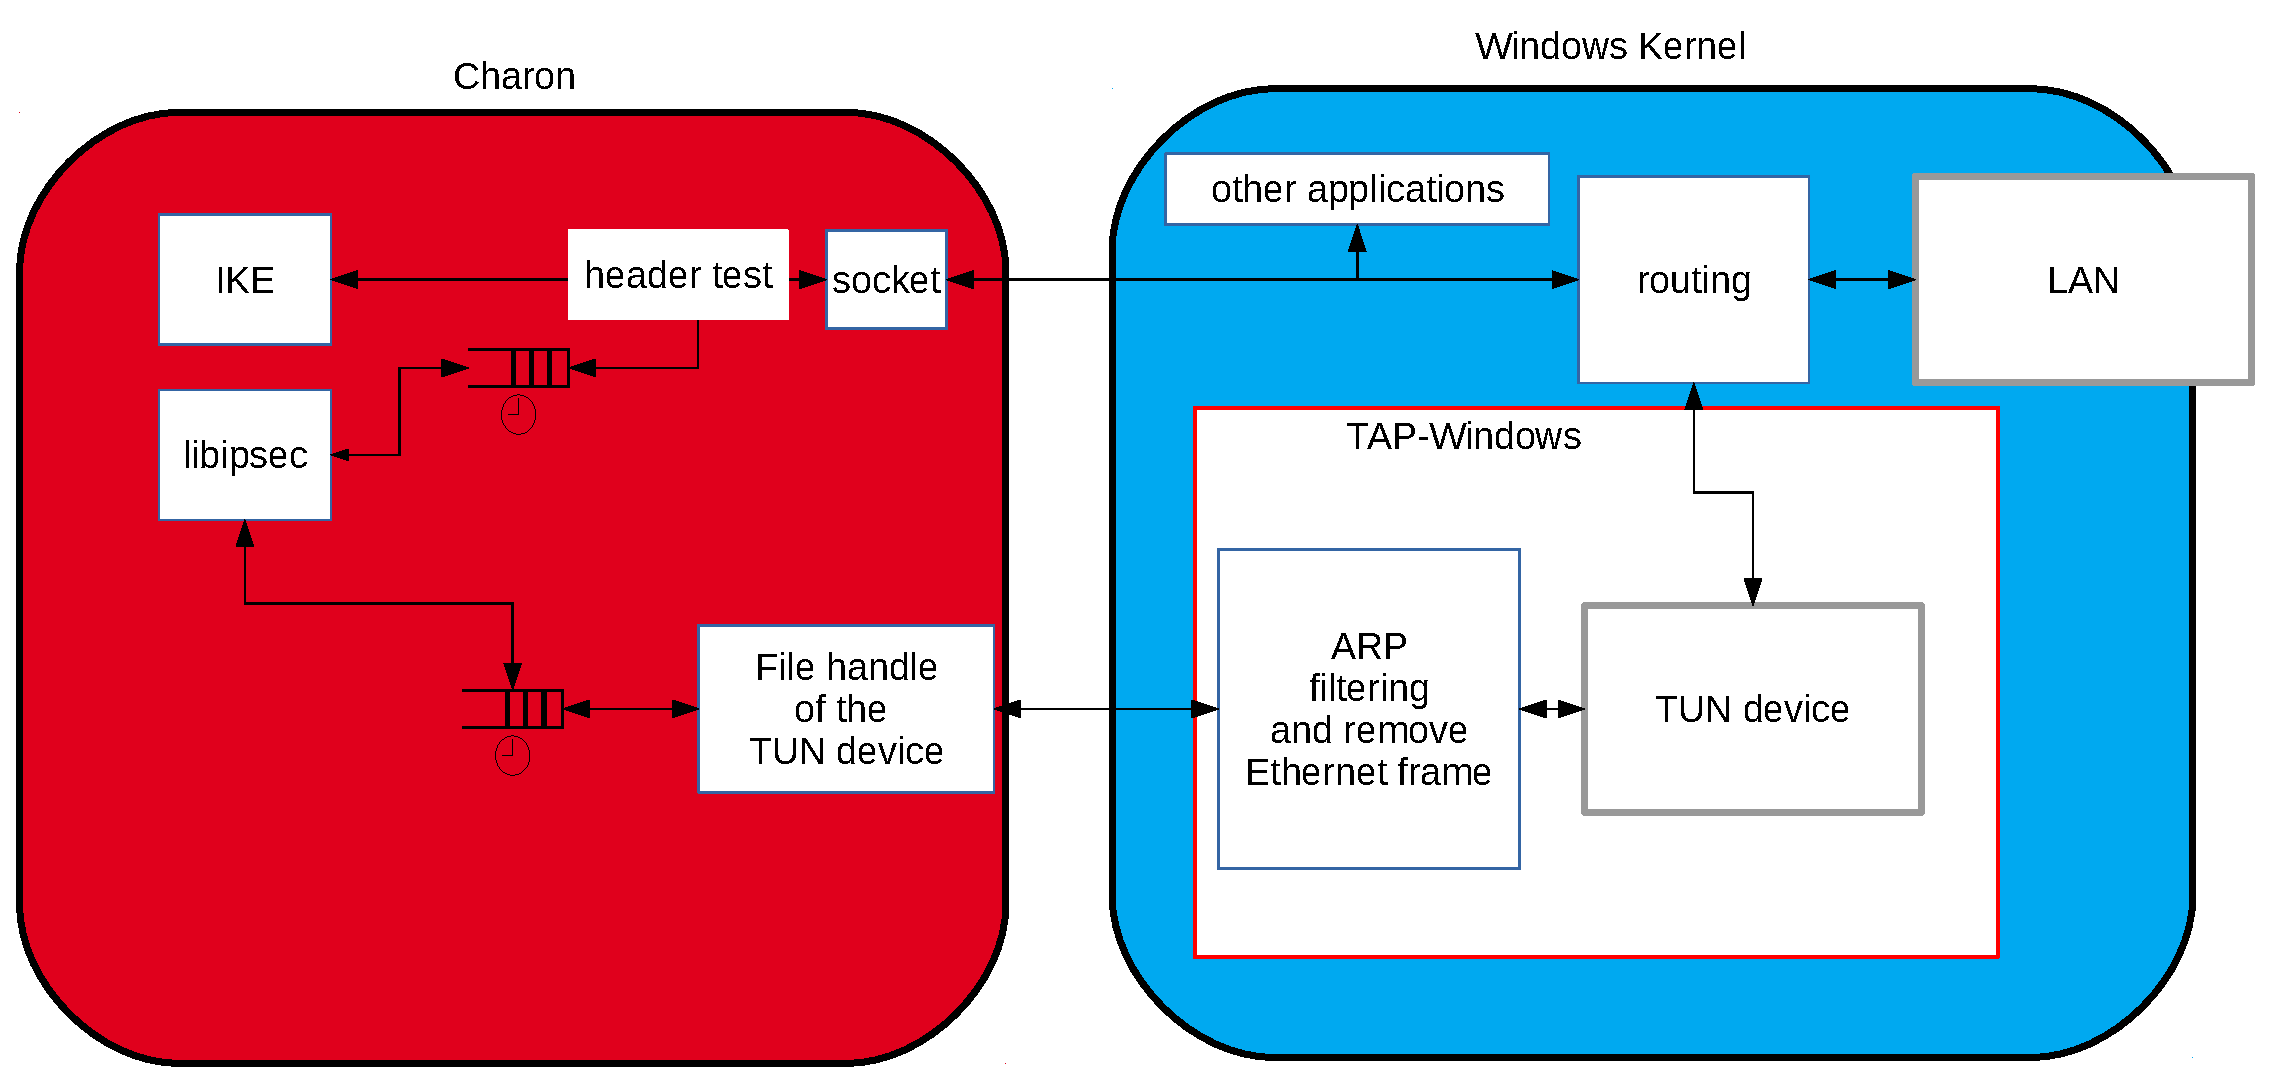
\includegraphics[width=\textwidth]{Diagram.eps}
\caption{Datenflussdiagramm}
\label{fig:Datenflussdiagramm}
\end{figure}

\subsection{Portierung von libipsec auf Windows}
Die Portierung von libipsec auf Windows, sodass sie dort lauffähig ist, ist das Ziel
der Bachelorarbeit. Die zu portierenden Teile des Programmcodes betreffen nur
die Codesegmente, die Plattformspezifische \acp{API} oder \acp{ABI} verwenden,
also primär alles um Dateiein- und Ausgabe, sowie das Verwalten von TUN-Geräten.
Unter Unix und Linux werden hier \acp{FD} verwendet. Unter Windows werden stattdessen
Handles genutzt, welche einen anderen Dateityp darstellen. Des weiteren unterscheidet
sich die Methode zum Multiplexen von Lese-Aufrufen auf einer Liste von Handles oder \acp{FD} stark.
Unter Unix und Linux wird hierfür poll() genutzt, unter Windows geschieht das jedoch
Event-basiert mit WaitForMultipleObjects().
Explizite Beispiele hierfür sind im Abschnitt über die Portierung von libipsec sichtbar.
Bei der Portierung wurde für das Verwalten von Speicherabschnitten 
primär alloca() genutzt, statt malloc() und seine Unterarten. Der Unterschied hierbei ist die
Speicherdauer. Mit alloca() allokierter Speicher ist nur bis zum Verlassen der Funktion gültig
und wird automatisch freigegeben. Mit malloc() allokierter Speicher muss manuell freigegeben werden.
alloca() ist ein Feature, welches nicht standardisiert ist.
Daher lässt sich strongSwan nicht mit allen C-Bibliotheken übersetzen.
Auf der Wiki-Seite über den Windows-Port wird erwähnt, dass nur die Kompilierung
mittels MinGW-W64 unterstützt wird.\footcite[][]{_windows_2015}


\subsection{Bestehende Implementierung}
Die bestehende Implementierung umfasst die eigentliche Bibliothek, eine Implementierung
eines Kernel-Interface zwischen libipsec und ''charon'', sowie Code in libstrongswan
um TUN-Geräte zu öffnen. Martin Willi hat 2014 bereits die gesamte Portierungsarbeit
für version 5.2.0 von strongSwan gemacht. Der Port unterstützt Windows 7 / server 2008 R2
und neuere Versionen von Microsoft Windows.

\subsection{Unterstützte Kryptographie}
Die unterstützte Kryptographie ist notwendigerweise von den deklarierten Identifikatoren
für IKE beschränkt. strongSwan unterstützt mehr Verschlüsselungsalgorithmen als
in den \acp{RFC} deklariert wurde. Aus diesem Grund nutzt strongSwan Identifikatoren
teilweise aus dem privaten Bereich, wenn die Identifikatoren für den eingesetzten Algorithmus
nicht standardisiert sind.

strongSwan unterstützt eine große Anzahl von Algorithmen im Vergleich zu anderen Implementierungen,
wie in den Tabellen in \autoref{sec:appendix} dagelegt wird. Wenn libipsec genutzt wird,
so können alle Algorithmen, die im Userspace implementiert sind, für die Absicherung
von Verkehr genutzt werden.

\subsection{Portierung}
\subsubsection{libipsec}
libipsec implementiert die Verarbeitung von Paketen, das Erzwingen der \acp{SP},
das Verwalten der \acp{SP}, \acp{SA}, Routen und der TUN-Geräte.
Die hierbei relevanten Dateien sind unter ''/src/libipsec/'' zu finden.

Standardmäßig installiert strongSwan die IP-Adressen die per Config-Mode
oder \ac{CP} empfangen wird auf dem ausgehenden Interface (Linux, Kernelspace processing),
was für die Kommunikation mit dem Peer genutzt wird,
oder auf dem Loopback-Adapter (Windows).
Um die IP-Adresse für TUN-Geräte korrekt zu setzen, nutzt libipsec den Parameter
''charon.install\_virtual\_ip\_on'' von strongswan.conf, der während der Initialisierung
des Plugins gesetzt wird.
% route installation
% queues
% processing
% event driven
% job
\paragraph{header}
Die Bibliotheken und Plugins um libipsec nutzen diverse Datenstrukturen und Konstanten,
die in C-Header-Dateien von Linux definiert sind. Diese sind unter Windows nicht verfügbar.
Aus diesem Grund wurde eine Kopie der relevanten Definitionen in den Quellcode kopiert
und fehlende Teile ergänz.
Spezifisch wurde aus dem Quellcode von GLIBC die Definition eines \ac{IP}v4-Headers
und eines \ac{IP}v6-Headers kopiert und die fehlenden Protokollkonstanten per Hand ergänzt.

Diese wurden in ''src/libipsec/win32.h'' abgelegt und in ''src/libpsec/ip\_packet.h'' und ''src/libipsec/ip\_packet.c''
inkludiert. Dies ist in diesem Fall nicht kritisch, da libipsec unter der GPLv2-Lizenz und
die Header unter der GPLv2 und der BSD-Lizenz stehen. Als Name für das Ifdef-Guard
wurde ''WINDOWS\_32\_PROTOCOL\_HEADERS'' gewählt.

\begin{lstlisting}[caption=Header für libipsec]
/* Copyright (C) 1991-2016 Free Software Foundation, Inc.
   This file is part of the GNU C Library.

   The GNU C Library is free software; you can redistribute it and/or
   modify it under the terms of the GNU Lesser General Public
   License as published by the Free Software Foundation; either
   version 2.1 of the License, or (at your option) any later version.

   The GNU C Library is distributed in the hope that it will be useful,
   but WITHOUT ANY WARRANTY; without even the implied warranty of
   MERCHANTABILITY or FITNESS FOR A PARTICULAR PURPOSE.  See the GNU
   Lesser General Public License for more details.

   You should have received a copy of the GNU Lesser General Public
   License along with the GNU C Library; if not, see
   <http://www.gnu.org/licenses/>.
*/

/*
 * Copyright (c) 1982, 1986, 1993
 *      The Regents of the University of California.  All rights reserved.
 *
 * Redistribution and use in source and binary forms, with or without
 * modification, are permitted provided that the following conditions
 * are met:
 * 1. Redistributions of source code must retain the above copyright
 *    notice, this list of conditions and the following disclaimer.
 * 2. Redistributions in binary form must reproduce the above copyright
 *    notice, this list of conditions and the following disclaimer in the
 *    documentation and/or other materials provided with the distribution.
 * 4. Neither the name of the University nor the names of its contributors
 *    may be used to endorse or promote products derived from this software
 *    without specific prior written permission.
 *
 * THIS SOFTWARE IS PROVIDED BY THE REGENTS AND CONTRIBUTORS ``AS IS'' AND
 * ANY EXPRESS OR IMPLIED WARRANTIES, INCLUDING, BUT NOT LIMITED TO, THE
 * IMPLIED WARRANTIES OF MERCHANTABILITY AND FITNESS FOR A PARTICULAR PURPOSE
 * ARE DISCLAIMED.  IN NO EVENT SHALL THE REGENTS OR CONTRIBUTORS BE LIABLE
 * FOR ANY DIRECT, INDIRECT, INCIDENTAL, SPECIAL, EXEMPLARY, OR CONSEQUENTIAL
 * DAMAGES (INCLUDING, BUT NOT LIMITED TO, PROCUREMENT OF SUBSTITUTE GOODS
 * OR SERVICES; LOSS OF USE, DATA, OR PROFITS; OR BUSINESS INTERRUPTION)
 * HOWEVER CAUSED AND ON ANY THEORY OF LIABILITY, WHETHER IN CONTRACT, STRICT
 * LIABILITY, OR TORT (INCLUDING NEGLIGENCE OR OTHERWISE) ARISING IN ANY WAY
 * OUT OF THE USE OF THIS SOFTWARE, EVEN IF ADVISED OF THE POSSIBILITY OF
 * SUCH DAMAGE.
 *
 *      @(#)ip.h        8.1 (Berkeley) 6/10/93
 */

/*
 * Details about licensing:
 * The definition of the IP header is from the headers of GLIBC, that come with Arch Linux
 * It is subject to the license headers of GLIBC and Berkeley
 * The IP protocol identifier constants are manually determined from /etc/protocols
 * and hand written out.  They are subject to the GPLv2.
 */

#ifndef WINDOWS_32_PROTOCOL_HEADERS
#define WINDOWS_32_PROTOCOL_HEADERS

/*
 * Structure of an internet header, naked of options.
 */
struct ip
  {
#if __BYTE_ORDER == __LITTLE_ENDIAN
    unsigned int ip_hl:4;               /* header length */
    unsigned int ip_v:4;                /* version */
#endif
    uint8_t ip_tos;                    /* type of service */
    u_short ip_len;                     /* total length */
    u_short ip_id;                      /* identification */
    u_short ip_off;                     /* fragment offset field */
#define IP_RF 0x8000                    /* reserved fragment flag */
#define IP_DF 0x4000                    /* dont fragment flag */
#define IP_MF 0x2000                    /* more fragments flag */
#define IP_OFFMASK 0x1fff               /* mask for fragmenting bits */
    uint8_t ip_ttl;                    /* time to live */
    uint8_t ip_p;                      /* protocol */
    u_short ip_sum;                     /* checksum */
    struct in_addr ip_src, ip_dst;      /* source and dest address */
  };

struct ip6_hdr
{
  union
    {
      struct ip6_hdrctl
        {
          uint32_t ip6_un1_flow;   /* 4 bits version, 8 bits TC,
                                      20 bits flow-ID */
          uint16_t ip6_un1_plen;   /* payload length */
          uint8_t  ip6_un1_nxt;    /* next header */
          uint8_t  ip6_un1_hlim;   /* hop limit */
        } ip6_un1;
      uint8_t ip6_un2_vfc;       /* 4 bits version, top 4 bits tclass */
    } ip6_ctlun;
  struct in6_addr ip6_src;      /* source address */
  struct in6_addr ip6_dst;      /* destination address */
};


#define ip6_vfc   ip6_ctlun.ip6_un2_vfc
#define ip6_flow  ip6_ctlun.ip6_un1.ip6_un1_flow
#define ip6_plen  ip6_ctlun.ip6_un1.ip6_un1_plen
#define ip6_nxt   ip6_ctlun.ip6_un1.ip6_un1_nxt
#define ip6_hlim  ip6_ctlun.ip6_un1.ip6_un1_hlim
#define ip6_hops  ip6_ctlun.ip6_un1.ip6_un1_hlim


#define IPPROTO_IPIP 4
#define IPPROTO_IPv6 41
#define IPPROTO_NONE 59

#endif /* WINDOWS_32_PROTOCOL_HEADERS */
\end{lstlisting}

\subsubsection{kernel-libipsec}
Die primäre Aufgabe hier war die Installation der Routen in ''kernel\_libipsec\_ipsec.c''
für Windows anzupassen, da hier ein Gateway verwendet wird auf einem TAP-Gerät
statt ein echtes TUN-Gerät, sowie die Anpassung des Codes für die Ein- und Ausgabe 
und einige Methoden in
''kernel\_libipsec\_router.c'', da das Multiplexen der Handles, sowie die Benachrichtigung
von anderen Threads auf Windows anders abläuft als auf Linux und UNIX.

\paragraph{Multiplexing}
Für das Multiplexen der Eingabe stehen unter Windows zwei Verfahren zur Verfügung:
\begin{itemize}
\item WaitForMultipleObjects
\item IOCompletionPorts
\end{itemize}

WaitForMultipleObjects\footcite[][]{_waitformultipleobjects_2016} funktioniert mit einem Array aus Handles. In der Struktur des Handles
ist das event-Attribut auf ein einzgartiges Event gesetzt, welches genutzt wird um
das Handle zu finden, dessen Lesevorgang abgeschlossen oder abgebrochen wurde.
Nach dem Kopieren des Handles in das Array und dem Setzen des Events wird ein asynchroner
Lesevorgang gestartet. Wenn er sofort beendet wurde, wird das entsprechende Event gesetzt.
Dadurch beendet der Aufruf von WaitForMultipleObjects() nach dem Aufruf direkt, falls
ein Lesevorgang schon zuvor erfolgreich war und der Programmcode wird etwas kürzer.
% Mehr Erläuterung benötigt

IOCompletionPorts\footcite[][]{_createiocompletionport_2016} funktionieren, indem man einen IOCompletionPort mit CreateIoCompletionPort()
anlegt und Handles mit ihm asoziiert. Bei der Asoziierung wird ein einzigartiger Schlüssel
übergeben, der bei der Signalisierung wieder zurückgegeben wird um das Handle identifizieren zu können.
Der CompletionPort kann erst nach dem Schließen der asoziierten Handles geschlossen werden.
Mit der Funktion GetQueuedCompletionStatus() kann der ausführende Thread dann auf abgeschlossene
I/O-Operationen warten.
Die Nachteile dieser Methode sind, dass jegliche Operationen auf den Handles eine Benachrichtigung
an GetQueuedCompletionStatus() generieren, obwohl Schreib-Vorgänge nicht von Interesse sind.

Des weiteren ähnelt die Nutzung von WaitForMultipleObjects() deren von poll()
insoweit, dass die Handles/\acp{FD} auch nach der Benutzung mit der Funktion
weiterhin einzeln genutzt werden können.
% Mehr Erläuterung benötigt

Da es relativ einfach ist WaitForMultipleObjects() zu nutzen, wurde diese Methode
für die Implementierung von handle\_plain() genutzt.

Die Zustände der Originalimplementierung sind in ~\autoref{fig:poll_fd}
dargestellt.

\begin{figure}
\centering
\def\svgwidth{\columnwidth}
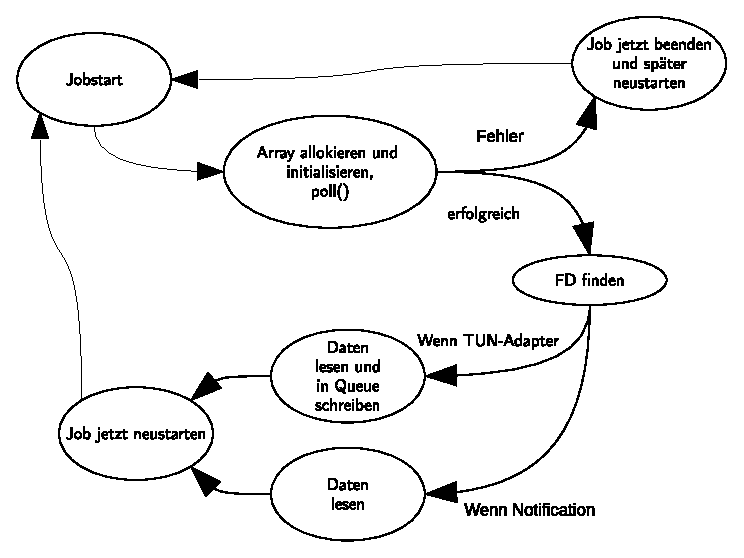
\includegraphics[width=\textwidth]{poll_fd.eps}
\caption{Zustände in handle\_plain() mittels poll()}
\label{fig:poll_fd}
\end{figure}


Wie aus dem Diagramm hervorgeht, wird im Prinzip nur ein Array mit Strukturen des Typs
''pollfd'' erstellt, dann mit einem Notification-\ac{FD} und den \acp{FD} der TUN-Geräte befüllt
und als gewünschte Events ''POLLIN'' gesetzt. Das heißt, dass der Aufruf von poll() ohne
Fehler beendet wird, wenn Daten auf dem \acp{FD} zur Verfügung stehen.
Danach wird poll() auf die ''pollfd''-Datenstruktur ausgeführt und analysiert,
auf welchen \acp{FD} Daten zur Verfügung stehen. Dieser Code ist relativ kurz im
Vergleich zum Analogon mit WaitFor*Objects() Funktionen unter Windows.
Dies geht aus den vergleichbaren Implementierungsmöglichkeiten, die sich aus den
WaitFor*Objects()-Funktionen ergeben. Dies wird im Diagramm \autoref{fig:WaitForMultipleObjects}
und \autoref{fig:WaitForMultipleObjects2} hervor. Diese Diagramme haben weitaus
mehr Zustände als \autoref{fig:poll_fd}.

Der Unterschied zwischen der Implementierung von \autoref{fig:WaitForMultipleObjects}
und \autoref{fig:WaitForMultipleObjects2} ist, dass \autoref{fig:WaitForMultipleObjects2}
effektiver und schneller ist, da die Puffer nach jedem Lesevorgang beibehalten werden
und IO-Operationen weiterlaufen können.
In \autoref{fig:WaitForMultipleObjects} werden die Puffer und Operationen
immer freigegeben und gestoppt. Das ist unnötig, bringt die Implementierung
jedoch näher an das Verhalten von \autoref{fig:poll_fd}.
Es wurde das Verfahren aus \autoref{fig:WaitForMultipleObjects2} implementiert,
da es schneller und effektiver ist.

In handle\_plain werden zwei verschiedene Arrays benutzt.
\begin{description}
\item[bundle\_array] Ein Array aus Strukturen vom Typ ''handle\_overlapped\_buffer\_t''. 
\item[event\_array] Ein Array aus Events (HANDLE).
\end{description}

Strukturen vom Typ ''handle\_overlapped\_buffer\_t'' beinhalten jeweils ein Objekt
vom Typ HANDLE, ein Objekt vom Typ *OVERLAPPED und ein Objekt vom Typ chunk\_t.
Das Handle gehört zu einem TUN-Handle, das OVERLAPPED-Objekt wird direkt für asynchrones
IO benötigt und das Objekt vom Typ chunk\_t beinhaltet den Pufferspeicher und dessen Länge.

Das ''event\_array'' Array zum Multiplexen mittels WaitForMultiplEvents() genutzt und
beinhaltet die gleichen Events, wie die Strukturen des Typs OVERLAPPED.
Bei der Ausführung von WaitForMultipleObjects() auf das Array wird darauf gewartet, dass
eine vorher gestartete Leseoperation auf einem Handle fertig gestellt wird.
Das signalisiert ein Event im Array und dessen Position im Array verrät welche
Position im bundle\_array einen nun gefüllten Puffer hat. Die Position signalisiert
hierbei nur die niedrigste Position im Array, deren Event signalisiert wurde. Ein
im Array höher gelegenes Event könnte auch signalisiert sein.
Der Puffer kann nun gelesen
werden und an die Queue zu libipsec gehängt werden. Nach dem Lesen wird die OVERLAPPED-Struktur
und das Event zurückgesetzt, sowie der Puffer mit Nullen initialisiert und die Länge zurückgesetzt.
Danach wird ein neuer Lesevorgang auf dem oder den Handles gestartet, deren Leseoperationen
fertig sind.

Der Code in auf Seite \pageref{lst:handle-plain-windows} zeigt die Implementierung von handle\_plain()
auf Windows. Die Funktionen zum Starten von asynchronen Leseoperationen auf Handles
wurden in start\_read() abgekapselt. Das Übersetzen von Fehlercodes in menschenlesbare
Texte wurde in format\_error() abgekapselt. Bei Fehlern beim Lesen startet sich der Job
mit JOB\_REQUEUE\_FAIR neu, sodass der Job als letzter vom Job-Manager in ''charon'' neugestartet wird,
wenn hoffentlich der Fehler nicht erneut auftritt.

\begin{figure}
\centering
\def\svgwidth{\columnwidth}
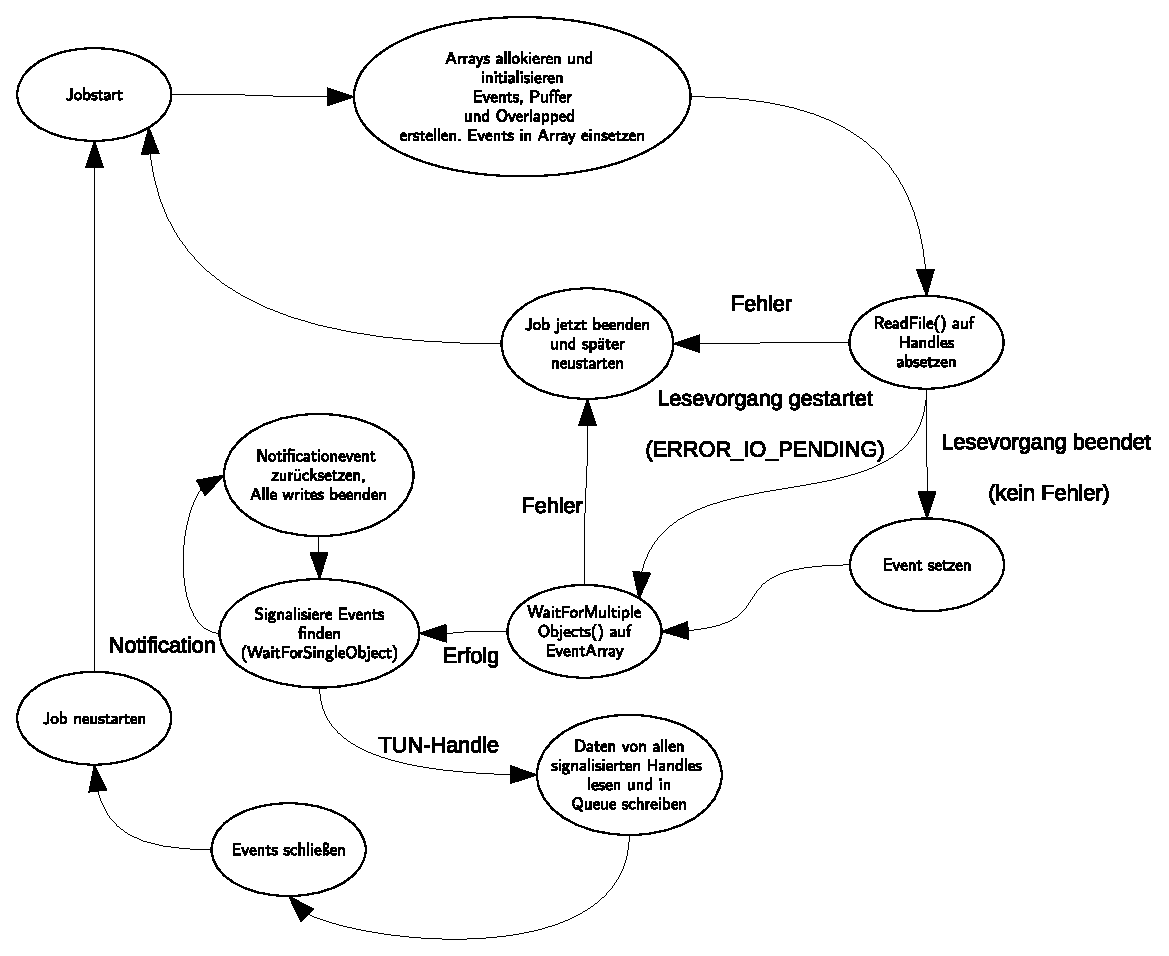
\includegraphics[width=\textwidth]{WaitForMultipleObjects.eps}
\caption{Zustände in handle\_plain() mittels WaitForMultipleObjects(), Variante 1}
\label{fig:WaitForMultipleObjects}
\end{figure}

\begin{figure}
\centering
\def\svgwidth{\columnwidth}
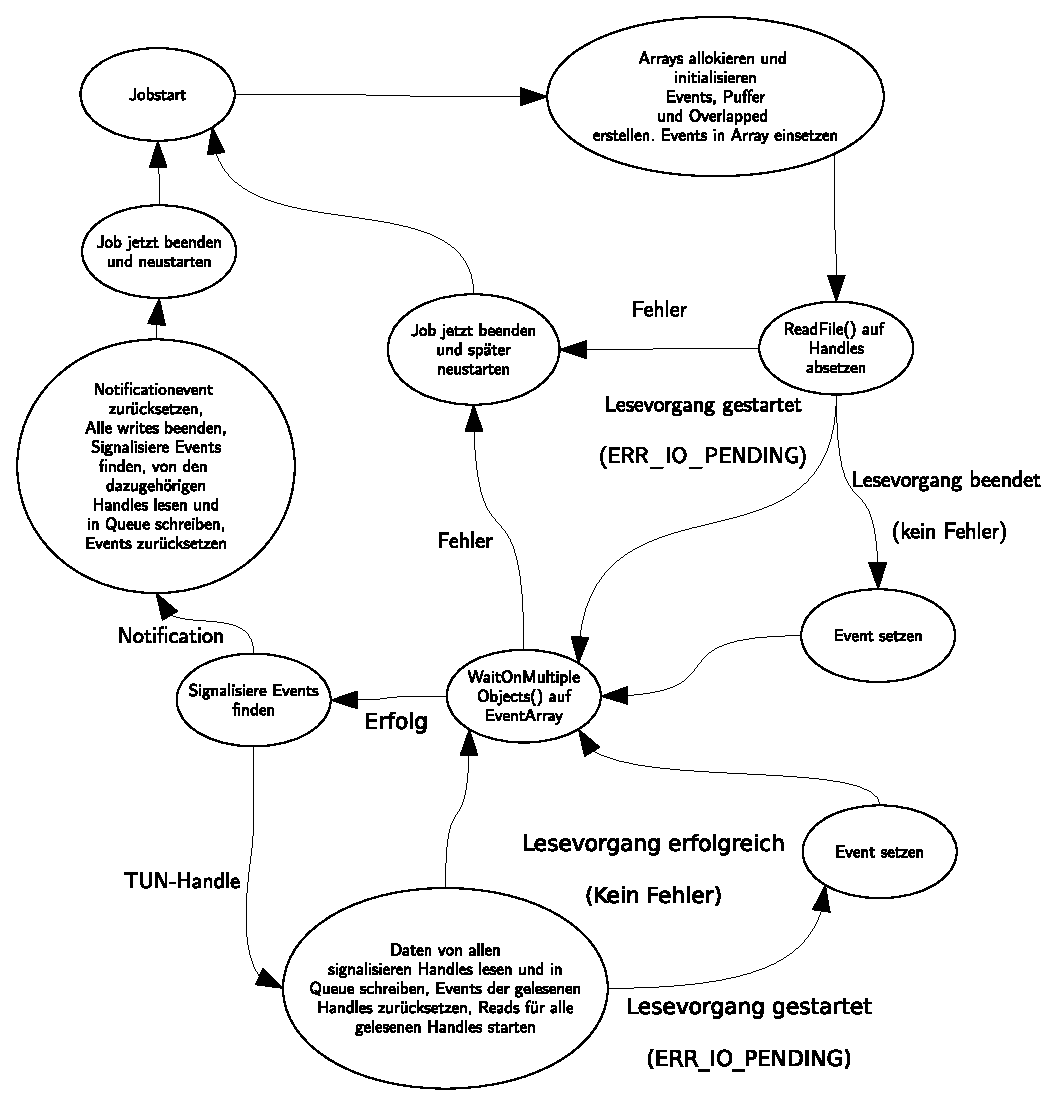
\includegraphics[width=\textwidth]{WaitForMultipleObjects2.eps}
\caption{Zustände in handle\_plain() mittels WaitForMultipleObjects(), Variante 2}
\label{fig:WaitForMultipleObjects2}
\end{figure}

\paragraph{Routing}
libipsec setzt für die von ihr installierten Routen standardmäßig das ''Gateway''
oder ''Next Hop''Feld nicht. Der Grund dafür ist, dass libipsec bisher nur auf
Betriebssytemen genutzt wurde, die echte Layer-3-Geräte implementieren und
daher keine Kollisionsdomäne über das Gerät erreichbar ist. Daher ergibt es keinen
Sinn das ''next hop''-Feld zu setzen.
Auf Windows ist dies jedoch, wie zuvor erläutert, nicht der Fall, da der TAP-Windows-Treiber
TUN-Geräte als Ethernet-Gerät emuliert.
Der Struct ''route'' is vom Typ ''route\_entry\_t'' und wird in der Funktion
''install\_route'' genutzt, um die zu installierende Route zu bestimmen.
Das Gateway-Feld wird genutzt, um das Next-Hop-Feld der Routen im Routing-Table
zu setzen. 
Der TAP-Windows6-Treiber nutzt für IPv6 einen statische IP addresse im link-local-Bereich
der IPv6-Spezifikation.
Für IPv4 lässt sich die IP-Adresse des Adapters implizit konfigurieren, wie zuvor erklärt.
Das Object, welches mittels ''host\_create\_from\_string'' erstellt wird,
wird von der Funktion auf dem Heap abgelegt. Damit ist es auch nach dem Verlassen
des Funktionsblocks noch valide. Es wird automatisch beim Zerstören des Objekts
''route'' freigegeben.

\begin{lstlisting}[caption=Patch für die Routen-Installation von libipsec]
#ifdef __linux__
#elif defined(WIN32)
        /* Set out special gateway */
        family = route->src_ip->get_family(route->src_ip);
        switch(family)
        {
            case AF_INET:
            {
                /* For IPv4, the nxt hop is 169.254.128.128 (Configured next hop) */
                host_t *gw = host_create_from_string("169.254.128.128", 0);
                route->gateway = gw;
                break;
            }
            case AF_INET6:
            {
                /* For IPv6, the next hop is fe80::8 (TAP-Windows6 magic router gw) */
                host_t *gw = host_create_from_string("fe80::8", 0);
                route->gateway = gw;
                break;
            }
            default:
                DBG2(DBG_ESP, "Unknown Protocol family %d encountered. Not setting a next hop.", family);
                break;
        }
#else
	/* on Linux we cant't install a gateway */
	route->gateway = charon->kernel->get_nexthop(charon->kernel, dst, -1, src);
#endif
\end{lstlisting}

Das Plugin ''kernel-iph'' installiert Routen mit einer Metrik von 10.
Andere Software von Windows, die Routen installiert, benutzen eine höhere Metrik.

Routen mit einer Prefixlänge von 0 werden auf zwei Routen mit der Prefixlänge 1 aufgeteilt.
Dies wird gemacht um die Standardroute, welche ebenfalls eine Metrik von 10 besitzt,
nicht zu überschreiben.

Die Implementierung von handle\_plain() auf Windows unterstütz, wie die Implementierung
auf Linux und UNIX das Multiplexen von IO von mehreren TUN-Adaptern. Der Grund dafür ist,
dass verschiedene TUN-Implementierungen gegebenenfalls verschiedene Adapter für mehrere Tunnel
benötigen. Mit dem TAP-Windows-Treiber ist dies zwar nicht der Fall, es wurde der Vollständigkeit
halber jedoch mitemplementiert.

% libipsec router
% handle_plain
% notification event
% job
% handle_plain
% handle_esp
% up
% destroy
%kernel_libipsec_ipsec route installation
\subsubsection{libstrongswan}
Hier galt es das Öffnen, Konfigurieren und Schließen von TUN-Geräten
mit dem TAP-Windows-Treiber zu implementieren.

% Bezugsquelle für den Treiber
Der Treiber ist kompiliert auf der OpenVPN-Seite
verfügbar\footnote{\url{https://openvpn.net/index.php/open-source/downloads.html}}
und der Quellcode auf Github\footnote{\url{https://github.com/OpenVPN}}.
Die Basis für die Implementierung war hier der existierende Programmcode in
OpenVPN, spezifisch in  der Datei ''src/openvpn/tun.c.''.

\paragraph{TAP-Geräte erstellen}
Das Erstellen von TAP-Geräten ist im Moment nicht unterstützt. Der Grund dafür ist,
dass die Funktionalität von ''devcon.exe'' dafür nachgebaut werden müsste.
Des weiteren ist der Quellcode von ''devcon.exe'' zwar verfügbar\footnote{\url{https://github.com/Microsoft/Windows-driver-samples/tree/master/setup/devcon}},
aber nur unter einer proprietären Lizenz von Microsoft, der MS-PL\footnote{\url{https://github.com/Microsoft/Windows-driver-samples/blob/master/LICENSE}},
verfügbar. Eine Reimplementierung müsste Code aus dem Quellcode von ''devcon.exe'' nutzen,
welcher dann auch unter der MS-PL stünde. Die Verbreitung des Codes wäre dann nicht möglich,
da die MS-PL mit der GPL inkompatibel ist\footnote{\url{https://www.gnu.org/licenses/license-list.en.html#GPLIncompatibleLicenses}}.
Da der Code unter der MIT-Lizenz beim strongSwan-Projekt eingereicht werden muss
und dann dual-lizensiert wird.
Wenn nur der Zugriff auf die benötigte API benutzt werden würde, so wäre es möglich,
die Unterstützung zu implementieren. Aus Zeitgründen wurde das nicht getan.

\paragraph{TAP-Geräte suchen}
Um das TAP-Gerät zu nutzen versucht der Code zuerst nach Netzwerkgeräten mit der ID ''tap0901'' zu suchen,
welche die ID für TAP-Geräte ist. Dies wird über die Registry getan. Hierbei wird
im Pfad \begin{lstlisting}[numbers=none]
HKEY_LOCAL_MACHINE\\SYSTEM\\CurrentControlSet\\Control\\Class\\{4D36E972-E325-11CE-BFC1-08002BE10318\}
\end{lstlisting}
nach Verbindungen gesucht, deren ''ComponentId''-Feld den Wert ''tap0901'' besitzen.
Bei passenden Schlüsseln wird der Wert ''NetCfgInstanceId'' an eine linked list
angehängt. Die NetCfgInstanceId identifiziert jeden Netzwerkadapter unter Windows
mittels einer einzigartigen ID.
Vor dem Beenden der Funktion wird die linked list zurückgegeben.
Diese Funktionalität ist in der Funktion get\_tap\_reg() in der Datei
''src/libstrongswan/networking/tun\_device.c'' gekapselt.

Der Code hierfür ist im Appendix unter \autoref{lst:get_tap_req} aufzufinden.

\paragraph{TAP-Geräte öffnen}
TAP-Geräte sind im Usermode über den Globalen Addressraum für Userspaceadapter
unter ''\textbackslash{}\textbackslash{}.\textbackslash{}\textbackslash{}Global\textbackslash{}\textbackslash{}\$NetCfgInstanceId.tap'' erreichbar.
''\$NetCfgInstanceId'' steht hierbei für die vorher mit ''get\_tap\_req()'' gefundenen
''NetCfgInstanceId''-Werte der gefundenen TAP-Adapter.

\begin{lstlisting}[numbers=none]
CreateFile(device_path, GENERIC_READ \| GENERIC_WRITE, 0,
                    0, OPEN_EXISTING, FILE_ATTRIBUTE_SYSTEM | FILE_FLAG_OVERLAPPED, 0);
\end{lstlisting}

Das Handle kann nun genutzt werden um Pakete vom TAP-Gerät zu lesen und zu schreiben.
Mittels DeviceIoControl kann die Konfiguration des Geräts geändert werden,
wie die IP des virtuellen Routers, den Status des Geräts sowie der Modus des Geräts.

Für die Portierung wurden die \acp{FD} für Handles ausgetauscht und für das Benachrichtigen
über Änderungen in der Liste der TUN-Geräte wurde ein Event verwendet.

Für das Lesen und Schreiben vom und auf dem Handle wird ein Event benötigt,
welches in die OVERLAPPED-Struktur eingefügt wird. Das Event wird dynamisch mittels CreateEvent()
erstellt und nach der Nutzung mittels CloseHandle() geschlossen.

\paragraph{Ändern der MTU eines TAP-Geräts}
Das Ändern der \ac{MTU} ist im Moment nicht unterstützt. Der Treiber ermöglicht es,
die \ac{MTU} über die Windows-Registry zu ändern. Dort wird der Schlüssel ''MTU''
dafür genutzt. Er steht standardmäßig auf ''1500'', welches die Standard-\ac{MTU}
von Ethernet ist.
\paragraph{Konfiguration eines TAP-Geräts}
Die Konfiguration eines TAP-Geräts geschieht mit den IOCTL-Werten aus ~/autoref{fig:tap-ioctls}.

Bei der Konfiguration eines TAP-Geräts für die Benutzung mit strongSwan müssen die folgenden
Schritte ausgeführt werden:
\begin{itemize}
\item Das Gerät in den TUN-Modus setzen. Dabei werden als Parameter
die lokale IP (169.254.128.127), die IP des virtuellen Routers (169.254.128.128)
und die Netzmaske des entfernten Netzwerks (255.255.255.255) gesetzt. 
(TAP\_WIN\_IOCTL\_CONFIG\_TUN)
\item Deaktivierung der Überprüfung des ''Sender protocol address''-Feldes.\\
(TAP\_WIN\_IOCTL\_CONFIG\_SET\_SRC\_CHECK)
\item Adapter in den ''up''-Zustand setzen (einschalten). 
Nach dem Setzen des Zustands muss kurz gewartet werden um sicher zu gehen, dass das Gerät auch aktiv ist.\\
(TAP\_WIN\_IOCTL\_SET\_MEDIA\_STATUS)
\end{itemize}

Folgend ist der Code für das Konfigurieren eines TAP-Geräts:
\begin{lstlisting}[caption=Konfiguration eines TAP-Geräts]
/**
 * Initialize the tun device
 */
static bool init_tun(private_tun_device_t *this, const char *name_tmpl)
[...]
#elif defined(WIN32)
        /* WIN32 TAP driver stuff*/
        /* Check if there is an unused tun device following the IPsec name scheme*/
        enumerator_t *enumerator;
        char *guid;
        BOOL success = FALSE;
        linked_list_t *possible_devices = get_tap_reg();
        memset(this->if_name, 0, sizeof(this->if_name));

        this->read_event_name = malloc(WIN32_TUN_EVENT_LENGTH);
        this->write_event_name = malloc(WIN32_TUN_EVENT_LENGTH);
        /* Iterate over list */
        enumerator = possible_devices->create_enumerator(possible_devices);
        /* Try to open that device */
        while(enumerator->enumerate(enumerator, &guid))
        {
            if (!success){
                /* Set mode */
                char device_path[256];
                /* Translate dev name to guid */
                /* TODO: Fix. device_guid should be */
                snprintf (device_path, sizeof(device_path), "%s%s%s", USERMODEDEVICEDIR, guid, TAP_WIN_SUFFIX);

                this->tunhandle = CreateFile(device_path, GENERIC_READ | GENERIC_WRITE, 0,
                    0, OPEN_EXISTING, FILE_ATTRIBUTE_SYSTEM | FILE_FLAG_OVERLAPPED, 0);
                if (this->tunhandle == INVALID_HANDLE_VALUE)
                {
                    DBG1(DBG_LIB, "could not create TUN device %s", device_path);
                }
                else
                {
                    memcpy(this->if_name, guid, strlen(guid));
                    success = TRUE;
                }
            }
            else
            {
                break;
            }
            /* device has been examined or used, free it */
            free(guid);
        }

        /* possible_devices has been freed while going over the enumerator.
         * Therefore it is not necessary to free the elements in the list now.
         */
        enumerator->destroy(enumerator);
        possible_devices->destroy(possible_devices);
        if (!success)
        {
            return FALSE;
        }
        /* set correct mode */
        /* We set a fake gateway of 169.254.254.128 that we route packets over
         The TAP driver strips the Ethernet header and trailer of the Ethernet frames
         before sending them back to the application that listens on the handle */
	struct in_addr ep[3];
        ULONG status = TRUE;
        DWORD len;
        /* Local address (just fake one): 169.254.128.127 */
	ep[0].S_un.S_un_b.s_b1 = 169;
        ep[0].S_un.S_un_b.s_b2 = 254;
        ep[0].S_un.S_un_b.s_b3 = 128;
        ep[0].S_un.S_un_b.s_b4 = 127;
        /*
         * Remote network. The tap driver validates it by masking it with the remote_netmask
         * and then comparing hte result against the remote network (this value here).
         * If it does not match, an error is logged and initialization fails.
         * (local & remote_netmask ? local)
         * The driver does proxy arp for this network and the local address.
         */
        /* We need to integrate support for IPv6, too. */
        /* Just fake a link local address for now (169.254.128.128) */
	ep[1].S_un.S_un_b.s_b1 = 169;
        ep[1].S_un.S_un_b.s_b2 = 254;
        ep[1].S_un.S_un_b.s_b3 = 128;
        ep[1].S_un.S_un_b.s_b4 = 128;
        /* Remote netmask (255.255.255.255) */
	ep[2].S_un.S_un_b.s_b1 = 255;
        ep[2].S_un.S_un_b.s_b2 = 255;
        ep[2].S_un.S_un_b.s_b3 = 255;
        ep[2].S_un.S_un_b.s_b4 = 255;

        if(!DeviceIoControl (this->tunhandle, TAP_WIN_IOCTL_CONFIG_TUN,
		    ep, sizeof (ep),
		    ep, sizeof (ep), &len, NULL))
        {
            DBG1 (DBG_LIB, "WARNING: The TAP-Windows driver rejected a TAP_WIN_IOCTL_CONFIG_TUN DeviceIoControl call.");
        }

        ULONG disable_src_check = FALSE;
        if(!DeviceIoControl(this->tunhandle, TAP_WIN_IOCTL_CONFIG_SET_SRC_CHECK,
                    &disable_src_check, sizeof(disable_src_check),
                    &disable_src_check, sizeof(disable_src_check), &len, NULL))
        {
            DBG1 (DBG_LIB, "WARNING: The TAP-Windows driver rejected a TAP_WIN_IOCTL_CONFIG_SET_SRC_CHECK DeviceIoControl call.");
        }
        ULONG driverVersion[3] = {0 , 0, 0};
        if(!DeviceIoControl(this->tunhandle, TAP_WIN_IOCTL_GET_VERSION,
                    &driverVersion, sizeof(driverVersion),
                    &driverVersion, sizeof(driverVersion), &len, NULL))
        {
            DBG1(DBG_LIB, "WARNING: The TAP-Windows driver rejected a TAP_WIN_IOCTL_GET_VERSION DeviceIoControl call.");
        }
        else
        {
            DBG1(DBG_LIB, "TAP-Windows driver version %d.%d available.", driverVersion[0], driverVersion[1]);
        }
        /* Set device to up */

        if (!DeviceIoControl (this->tunhandle, TAP_WIN_IOCTL_SET_MEDIA_STATUS,
  			  &status, sizeof (status),
                            &status, sizeof (status), &len, NULL))
        {
            DBG1 (DBG_LIB, "WARNING: The TAP-Windows driver rejected a TAP_WIN_IOCTL_SET_MEDIA_STATUS DeviceIoControl call.");
        }

            /* Give the adapter 2 seconds to come up */
        /* Create event with special template */
        snprintf(this->read_event_name, WIN32_TUN_EVENT_LENGTH, WIN32_TUN_READ_EVENT_TEMPLATE, this->if_name);
        snprintf(this->write_event_name, WIN32_TUN_EVENT_LENGTH, WIN32_TUN_WRITE_EVENT_TEMPLATE, this->if_name);
        sleep(2);
        return TRUE;
        [...]
}
\end{lstlisting}

\paragraph{Lesen und Schreiben vom Adapter}
Beim Öffnen des Adapters wurde ein Handle erstellt.
Durch asynchrone Lese- und Schreiboperationen mittels ReadFile() und WriteFile()
unter Benutzung von ''OVERLAPPED''-Strukturen und Events lassen sich Pakete
lesen und schreiben.

\paragraph{tun\_device\_t}
Folgend der Code für das Erstellen eines Objects vom Typ ''tun\_device\_t''.

\begin{lstlisting}[caption=Code für das Erstellen von tun\_device\_t]
/*
 * Described in header
 */
tun_device_t *tun_device_create(const char *name_tmpl)
{
	private_tun_device_t *this;

	INIT(this,
		.public = {
			.read_packet = _read_packet,
			.write_packet = _write_packet,
			.get_mtu = _get_mtu,
			.set_mtu = _set_mtu,
			.get_name = _get_name,
                        /* For WIN32, that's a handle. */
#ifdef WIN32
                        .get_handle = _get_handle,
                        .get_write_event_name = _get_write_event_name,
                        .get_read_event_name = _get_read_event_name,
#else
			.get_fd = _get_fd,
#endif /* WIN32 */
			.set_address = _set_address,
			.get_address = _get_address,
			.up = _up,
			.destroy = _destroy,
		},
#ifdef WIN32
                .tunhandle = NULL,
#else
		.tunfd = -1,
		.sock = -1,
#endif /* WIN32 */
	);

	if (!init_tun(this, name_tmpl))
	{
		free(this);
		return NULL;
	}
	DBG1(DBG_LIB, "created TUN device: %s", this->if_name);

#ifdef WIN32
#else
	this->sock = socket(AF_INET, SOCK_DGRAM, 0);
	if (this->sock < 0)
	{
		DBG1(DBG_LIB, "failed to open socket to configure TUN device");
		destroy(this);
		return NULL;
	}
#endif /* WIN32 */
	return &this->public;
}

#endif /* TUN devices supported */
\end{lstlisting}

\begin{lstlisting}[caption=Relevanter code für tun\_device\_t->destroy()]
METHOD(tun_device_t, destroy, void,
	private_tun_device_t *this)
{
#ifdef WIN32
        /* close file handle, destroy interface */
        CloseHandle(this->tunhandle);
        free(this->read_event_name);
        free(this->write_event_name);
#else
        [...]
#endif
    	DESTROY_IF(this->address);
    	free(this);
}
\end{lstlisting}
% callbacks
% synchronous
% WaitForMultipleObjects
% komplexe Änderungen des Verhaltens von kernel-libipsec

\subsubsection{kernel-iph}
kernel-iph ist ein Plugin für ''charon'', das das Kernel-Interface
für die Verwaltung von IP-Adressen und Routen implementiert.

Ursprünglich war das Verwalten von IP-Adressen im Master-Zweig nicht implementiert.
Eine vollständige Implementierung existiert im Zweig ''win-vip'', die in den Zweig 'windows-libipsec'
gemerged wurde, um eine vollständige Implementierung dort zu erhalten.

Nachgerüstet werden musste Code zum Beachten des ''charon.install\_virtual\_ip\_on'' Parameters
der in der Datei ''strongswan.conf'' definiert werden kann und den libipsec nutzt um
die Installation der empfangenen IP-Adresse(n) auf den richtigen Adapter zu erzwingen.
Der Code kopiert den Adapternamen während der Initialisierung des Plugins, daher
ändert ein Ändern des Parameters während der Laufzeit nicht die Schnittstelle,
auf die die IP-Adresse installiert werden würde.

Die bekannten IP-Adressen werden in kernel-iph in einer Datenstruktur gespeichert,
um sie schnell nachschlagen zu können und Berechnungen zu tätigen. Die Struktur
wird einerseits durch manuelles Einfügen und Entfernen von selbstinstallierten Adressen
bewerkstelligt, als auch durch Events, die die Anwendung über ein Handle
vom Kernel empfängt.

\begin{lstlisting}[caption=Ergänzung zu private\_kernel\_iph\_net\_t]
/**
 * Private data of kernel_iph_net implementation.
 */
struct private_kernel_iph_net_t {
        [...]
        /**
         * Whether to install virtual IPs
         */
        bool install_virtual_ip;

        /**
         * Where to install virtual IPs
         */

        char *install_virtual_ip_on;
};
\end{lstlisting}

\begin{lstlisting}[caption=Code für add\_ip]
METHOD(kernel_net_t, add_ip, status_t,
	private_kernel_iph_net_t *this, host_t *vip, int prefix, char *name)
{
	if (!this->install_virtual_ip)
	{	/* disabled by config */
		return SUCCESS;
	}
	MIB_UNICASTIPADDRESS_ROW row;
	u_long status;
        iface_t *iface = NULL, *entry = NULL;

        /* Print out all known interfaces */
        enumerator_t *enumerator = this->ifaces->create_enumerator(this->ifaces);
        while(enumerator->enumerate(enumerator, &entry))
        {
            DBG1(DBG_KNL, "interface %s\n index: %d\n description %s\n type %d", entry->ifname, entry->ifindex, entry->ifdesc, entry->iftype);
        }
        enumerator->destroy(enumerator);
	/* name of the MS Loopback adapter */
        if (!this->install_virtual_ip_on || this->ifaces->find_first(this->ifaces, (void*)iface_by_name,
						(void**)&iface, this->install_virtual_ip_on) != SUCCESS)
        {
            name = "{DB2C49B1-7C90-4253-9E61-8C6A881194ED}";
        }
        else
        {
            name = this->install_virtual_ip_on;
        }
	host2unicast(vip, prefix, &row);

	row.InterfaceIndex = add_addr(this, name, vip, TRUE);
	if (!row.InterfaceIndex)
	{
		DBG1(DBG_KNL, "interface '%s' not found", name);
		return NOT_FOUND;
	}

	status = CreateUnicastIpAddressEntry(&row);
	if (status != NO_ERROR)
	{
		DBG1(DBG_KNL, "creating IPH address entry failed: %lu", status);
		remove_addr(this, vip);
		return FAILED;
	}
	return SUCCESS;
}
\end{lstlisting}

\begin{lstlisting}[caption=Code für del\_ip]
METHOD(kernel_net_t, del_ip, status_t,
	private_kernel_iph_net_t *this, host_t *vip, int prefix, bool wait)
{
        if (!this->install_virtual_ip)
	{	/* disabled by config */
		return SUCCESS;
	}

	MIB_UNICASTIPADDRESS_ROW row;
	u_long status;

	host2unicast(vip, prefix, &row);

	row.InterfaceIndex = remove_addr(this, vip);
	if (!row.InterfaceIndex)
	{
		DBG1(DBG_KNL, "virtual IP %H not found", vip);
		return NOT_FOUND;
	}

	status = DeleteUnicastIpAddressEntry(&row);
	if (status != NO_ERROR)
	{
		DBG1(DBG_KNL, "deleting IPH address entry failed: %lu", status);
		return FAILED;
	}

	return SUCCESS;
}
\end{lstlisting}

\begin{lstlisting}[caption=Ergänzung zu kernel\_iph\_net\_create()]
*
 * Described in header.
 */
kernel_iph_net_t *kernel_iph_net_create()
{
        [...}
		.install_virtual_ip = lib->settings->get_bool(lib->settings,
						"%s.install_virtual_ip", TRUE, lib->ns),
		.install_virtual_ip_on = lib->settings->get_str(lib->settings,
						"%s.install_virtual_ip_on", NULL, lib->ns),
	   [...]
}
\end{lstlisting}

Für das Implementieren des Codes für den TAP-Treiber werden Magic Numbers benötigt,
welche sich im Quellcode von OpenVPN finden lassen. Diese wurden übernommen
und in einer Header-Datei angelegt.
Teilweise wurden auch die Konstanten für die Erzeugung der Namen der Events für
das IO-Multiplexen dort abgelegt. Die Datei ist im Appendix unter \autoref{lst:libstrongswan-win32.h}
zu finden.

Der gesamte gepatchte Quellcode von strongSwan ist auf der CD unter strongSwan/ zu finden
Der Patch ansich ist unter patches/strongSwan/tap-handling.patch zu finden.

\subsection{TAP-Treiber}
% openvpn
% kompatibilität
% Treiber-patches upstream
Im Zuge der \ac{BA} wurde ein Patch für den TAP-Windows-Treiber entwicklelt, um die
Prüfung der Quell-IP der ARP-Requests zu deaktivieren. Das ist erforderlich, um mit der
virtuellen IP des Clients mit dem entfernten IP-Netzwerk kommunizieren zu können.


\subsubsection{Bauen und Installieren des Treibers}
Um den Treiber zu bauen, wird zuallererst der Quellcode benötigt, sowie die
Vorraussetzungen, welche auf der Github-Seite dort aufgelistet sind.
Die aktuellen Minimalvorraussetzungen sind Python 2.7, das Microsoft Windows 7 WDK (Windows Driver Kit)
und ein Windows Code signing certificate.
Das Zertifikat muss nicht valid sein, wenn der Treiber nicht produktiv ausgerollt
werden soll. Der Grund ist, dass unter Windows das Überprüfen der Treibersignatur deaktiviert
werden kann, aber der Treiber muss trotzdem signiert sein. Der Trust-path muss aber nicht
zu einem öffentlichen Trust Anchor (eine CA) führen. Um den Treiber signieren zu können,
wird die gesamte Trust Chain benötigt, sowie der private Schlüssel des Zertifikats.
Um ein Zertifikat mit dem dazugehörigen privaten Schlüssel importieren zu können,
müssen die Dateien in einen PKCS\#12-Container gepackt werden. Dieser kann mit 
OpenSSL erstellt werden, zum Beispiel mit diesem Befehl:
\begin{lstlisting}[caption=OpenSSL PKCS\#12]
openssl pkcs12 -export -in key key.key -in certificate.pem -out pkcs12.p12
\end{lstlisting}
Die mit diesem Befehl erstellte Datei pkcs12.p12 kann dann durch einen Doppelklick auf sie
in den Windows importiert werden.

Der Befehl um den Treiber dann zu bauen kann so aussehen:
\begin{lstlisting}[caption=TAP-Windows bauen]
python buildtap.py -c -b -d --cert="csc" --sign --crosscert="C:\Users\Noel\certs\rootca.pem"
\end{lstlisting}
Die Ausgabe des Befehls listet die Kompilierung, sowie das Signieren der Dateien auf.
% Hier noch Ausgabe der Kompilierung aufführen, sowie welche Teile kritisch sind.
Wie zu sehen ist, muss das Root-CA-Zertifikat als Datei vorhanden sein.
Das Code Signing certificate wird nur mit seinem Common Name angegeben.
Damit das WDK es findet, muss es in ''Eigene Zertifikate'' zu finden sein.
\begin{figure}
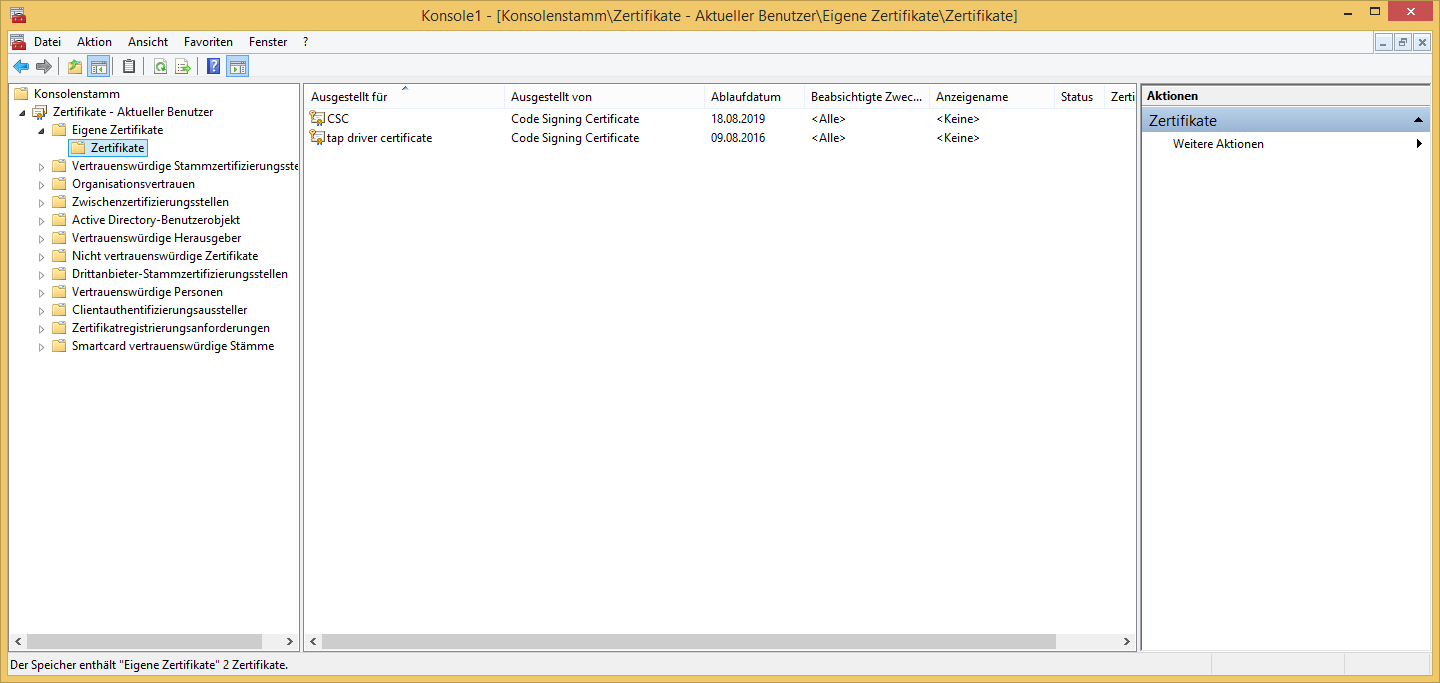
\includegraphics[scale=0.33]{/home/thermi/FH-Stuff/UNITS-8/Bachelorarbeit/Bachelorarbeit/Bilder/Eigene_Zertifikate.png}
\caption{Eigene-Zertifikate-Menü}
\label{fig:Eigene-Zertifikate-Menue}
\end{figure}

Mit Windows im Testmodus kann der Treiber geladen werden und TAP-Geräte konnen
mittels tapinstall.exe (Was eigentlich ''devcon.exe'' ist). Die Datei ist im Quellcode des
Treibers nicht mitenthalten. Sie kann jedoch durch die Installation des Treiber-Pakets
von der OpenVPN-Webseite erhalten werden. Nach der Installation des Pakets
ist die Datei unter \textit{C:\textbackslash{}Program Files\textbackslash{}TAP-Windows\textbackslash{}bin\textbackslash{}tapinstall.exe}
zu finden und kann zur Erstellung und zum Löschen von TAP-Geräten genutzt werden.

Der erste Parameter ist offensichtlich ''install'' oder ''remove''. Der Pfad zur .inf-Datei
über den Treiber muss beim Erstellen eines Geräts angegeben werden. Hier im Beispiel
ist es die Datei, die mittels des Python-Skripts erstellt wurde. Bei der Installation
dieses Treibers wird der von mir kompilierte Treiber installiert, welcher sich unter 
''C:\textbackslash{}Users\textbackslash{}Noel\textbackslash{}tap-driver\textbackslash{}dist\textbackslash{}amd64\textbackslash{}OemVista.inf''
befindet.

\begin{lstlisting}[caption=Erstellung eines TAP-Geraets]
"C:\Program Files\TAP-Windows\bin\tapinstall.exe" install "C:\Users\Noel\tap-driver\dist\amd64\OemVista.inf" tap0901
\end{lstlisting}

\begin{lstlisting}[caption=Löschung aller TAP-Geraete]
"C:\Program Files\TAP-Windows\bin\tapinstall.exe" remove tap0901
\end{lstlisting}

\paragraph{ABI}
Die \ac{ABI} des Treibers ist undokumentiert. Im Folgenden ist eine Auflistung
der Funktionen der \ac{ABI}. Sie wurden aus der Datei ''src/device.c'' extrahiert
und aufgeschlüsselt. Für mehr Informationen bezüglich des Verhaltens und der
genauen Eingabeparameter sollte die Datei konsultiert werden.

\begin{table}
\tiny
\begin{tabularx}{\textwidth}{|c|c|c|c|X|X|}\firsthline
IOCtl & Makro & Eingabe & Ausgabe & Zweck & Kommentar \\ \hline
1 & TAP\_WIN\_IOCTL\_GET\_MAC & NULL & char[6] & Gibt die MAC-Adresse des Geräts zurück & \\ \hline
2 & TAP\_WIN\_IOCTL\_GET\_VERSION & NULL & ULONG[3] & Gibt die Version des Treibers zurück & \\ \hline
3 & TAP\_WIN\_IOCTL\_GET\_MTU & NULL & ULONG & Gibt die \ac{MTU} des Geräts zurück & \\ \hline
4 & TAP\_WIN\_IOCTL\_GET\_INFO & NULL & N/A & Gibt Informationen über den Adapter zurück
& Ist laut Code für NDIS6 nicht implementiert \\ \hline 
5 & TAP\_WIN\_IOCTL\_CONFIG\_POINT\_TO\_POINT & IPADDR[2] (2*4 CHAR) & NULL & Setzt das Gerät in den Point-To-Point-Modus
& \\ \hline
6 & TAP\_WIN\_IOCTL\_SET\_MEDIA\_STATUS & ULONG & NULL & Setzt das Gerät in den ''Up'' oder ''Down''-Zustand & \\ \hline
7 & TAP\_WIN\_IOCTL\_CONFIG\_DHCP\_MASQ & IPADDR[4] (4*4 CHAR) & NULL & Aktiviert den internen DHCP-Server, DHCP-IP-Adresse, DHCP-Netzmaske, DHCP-Server-IP, Leasetime & \\ \hline
8 & TAP\_WIN\_IOCTL\_GET\_LOG\_LINE & allokierter String (char *) & NULL & Gibt eine Debug-Log-Zeile zurück & \\ \hline
9 & TAP\_WIN\_IOCTL\_CONFIG\_DHCP\_SET\_OPT & char[256] & NULL & Setzt die DHCP-Optionen & \\ \hline
10 & TAP\_WIN\_IOCTL\_CONFIG\_TUN & IPADDR[3] (3*4 char) & NULL & Setzt das Gerät in den TUN-Modus, lokale IP, entferntes Netzwerk, entfernte Netzmaske & \\ \hline
11 & TAP\_WIN\_IOCTL\_CONFIG\_SET\_SRC\_CHECK & ULONG & NULL & Deaktiviert oder Aktiviert den ARP-Source-Check. ''0'' deaktiviert ihn. ''1'' aktiviert ihn (Standard) & \\ \hline
\end{tabularx}
\caption{TAP-Windows-Treiber IOCtls}
\label{fig:tap-ioctls}
\end{table}

\paragraph{Patch}
Bei der Entwicklung des Patchs wurde viel Zeit darauf verwendet die funktionalen
Komponenten zu finden, die bei der Verarbeitung von \ac{ARP}-Requests ausgeführt werden,
sowie die Codepfade zu finden, die bei der Verarbeitung von Daten abgelaufen werden.

Der entwickelte Patch deaktiviert die Überprüfung der Quell-IP der \ac{ARP}-Requests, die
vom Treiber verarbeitet werden. Wenn die Überprüfung erfolgreich war, so wird der ARP-Request
beantwortet und dem Kernel wird damit mitgeteilt, wie die MAC-Adresse des virtuellen Routers lautet.

Für die Implementierung der Routen wurde die Nutzung eines virtuellen Routers gewählt,
da das Routen aller \ac{IP}-Adressen über das Gerät die \ac{ARP}-Tabelle des Clients
mehr gefüllt hätte und eine \ac{ARP}-Adressabfrage bei jeder Kommunikation mit einer neuen
\ac{IP}-Adresse zu Folge hätte.

Der Patch wurde entwickelt, indem nach der Behandlung von \ac{ARP}-Paketen im
Quellcode des Treibers gesucht wurde. Dafür wurde nach ''ARP'' und ''arp'' mittels
''grep'' im Quelltext gesucht. Dabei wurde die Funktion ''ProcessARP'' in ''src/txpath.c''
gefunden, in der \ac{ARP}-Requests verarbeitet werden. In dieser Funktion
werden verschiedene Felder des Pakets überprüft, unter anderem das ''Sender protocol address''-Feld.

Die Überprüfung des ''Sender protocol address''-Felds wurde optional gemacht, 
wobei es standardmäßig aktiviert ist. Die Kontrolle dieses
Feldes kann über ein IOCTL-Wert gesteuert werden. Der momentane Zustand der Option
wird im Adapter-Kontext des TAP-Adapters gespeichert.

Er wurde 2016-08-15 in der OpenVPN Community auf freenode im Kanale \#openvpn-meeting besprochen
und bekam ein feature-ack. Ein Code-ack steht noch aus. Das Ticket ist unter
\url{https://community.openvpn.net/openvpn/ticket/721} zu finden.

Der komplette Patch ist auf der CD unter 
''patches/tap-windows/0001-implement-source-ip-check.patch'' zu finden.


\subsection{Test des Codes}
Zum Konfigurieren und Bauen des Quellcodes wurde der folgende Befehl verwendet.
Im Testszenario wurde der Quellcode auf Linux für Windows 64-Bit cross kompiliert
und in einer \ac{VM} mit Windows 8.1 ausgeführt.
Die gebauten Binärdateien wurden über ein geteiltes Verzeichnis der \ac{VM}
zugänglich gemacht. Danach wurden sie in ''C:\textbackslash{}\textbackslash{}Users\textbackslash{}\textbackslash{}Thermi\textbackslash{}\textbackslash{}bin
kopiert und in 'cmd' mit Administratorrechten ausgeführt. 
Die nötige Dateistruktur sollte wie in Abbildung \ref{fig:Ordnerstruktur} 
auf Seite \pageref{fig:Ordnerstruktur} aussehen.

Im Unterordner ''swanctl'' befindet sich die Dateien ''swanctl.conf'',
sowie die Ordner ''bliss'', ''ecdsa'', ''pkcs8'', ''pkcs12'', ''pubkey'', ''rsa'', ''x509'',
''x509aa'', ''x509ac'', ''x509ca'', ''x509crl'' und''x509ocsp''.
Im Ordner ''rsa'' befindet sich der private Schlüssel für den Client. Im Ordner
''x509'' befindet sich das Zertifikat des Clients und im Ordner ''x509ca'' alle
\ac{CA}-Zertifikate vom Zertifikat des Clients bis zum selbstsignierten Wurzelzertifikat,
sowie das Zertifikat der Server-\ac{CA}.

\begin{figure}
\def\svgwidth{\columnwidth}
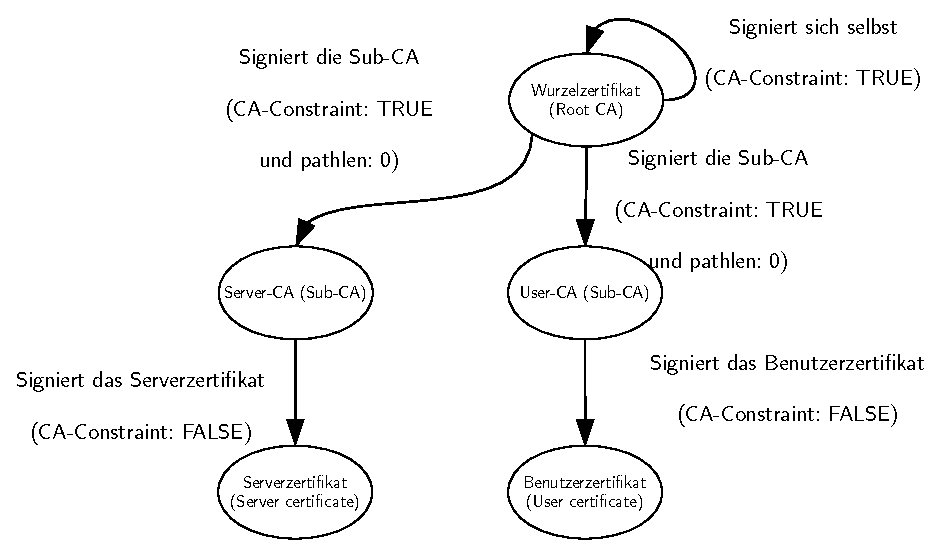
\includegraphics[width=\textwidth]{CA-Struktur.eps}
\caption{Eine exemplarische CA-Struktur}
\label{fig:CA-Struktur}
\end{figure}

Die Datei ''this\_log'' wurde von der Logger-Konfiguration des Dienstes erstellt.
Hierbei wurde zuerst ''charon-svc.exe''
in einem ersten Fenster ausgeführt. In einem zweiten Fenster wurde die Konfiguration geladen
und der Tunnelaufbau mittels ''swanctl.exe'' gestartet. Hierbei wurden die folgenden
Befehle verwendet: ''swanctl.exe --load-all'' und ''swanctl --i --child bar''.
Nach dem Testen wurde der Tunnel, sollte ''charon-svc.exe'' nicht gecrasht sein, mit ''swanctl -t --ike foo''
beendet, sodass keine virtuellen IP-Adressen oder Routen für den nächsten Test zurückbleiben.

Wenn ''charon-svc.exe'' getötet wird, während ein Tunnel mit Routen und \ac{IP}-Adressen
aufgebaut ist, so verbleiben IP-Adressen und Routen auf dem Adapter, was verhindern kann dass
dieselben Routen und \ac{IP}-Adressen wieder installiert werden. Das führt dazu, dass der
Aufbau der CHILD\_SA fehlschlägt und ein neuer Tunnel nicht aufgebaut werden kann.
In diesem Fall müssen sie manuell über die Nutzung von ''route delete'' oder ''netsh''
gelöscht werden oder Windows neu gestartet werden.

OpenSSL auf Windows wird für die Kryptographie benötigt und liegt nicht in den Standardsuchpfaden
für Bibliotheken und Header. Aus diesem Grund werden die Header und Bibliotheken
über LDFLAGs in Include-Pfade auf der Kommandozeile übergeben.

Die Bibliotheken von OpenSSL wurden durch die Installation von OpenVPN beschafft.
Bei der Installation von OpenVPN werden direkt die Bibliotheken von openssl mitinstalliert.

\begin{centering}
\begin{figure}
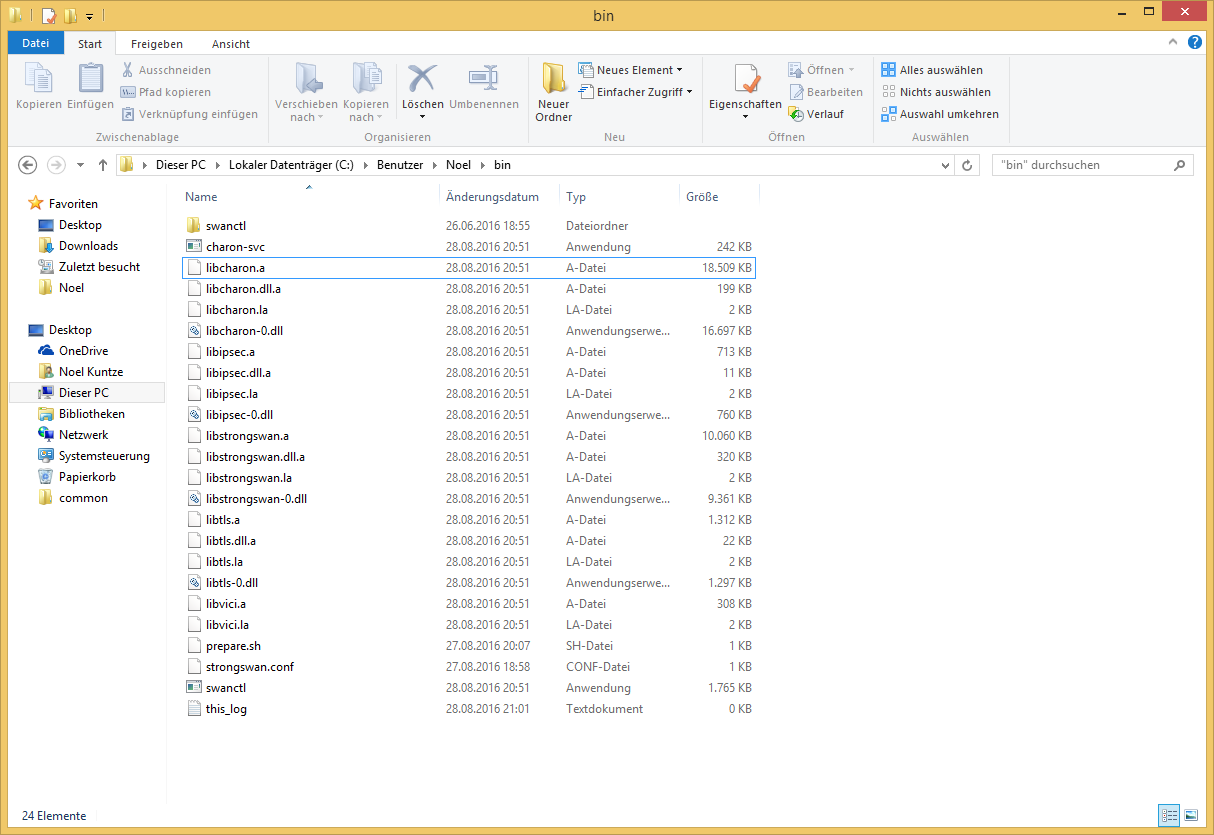
\includegraphics[width=\textwidth]{Bilder/Ordnerstruktur.png}
\caption{Ordnerstruktur nach dem Kopieren der Dateien}
\label{fig:Ordnerstruktur}
\end{figure}
\end{centering}

\begin{centering}
\begin{figure}
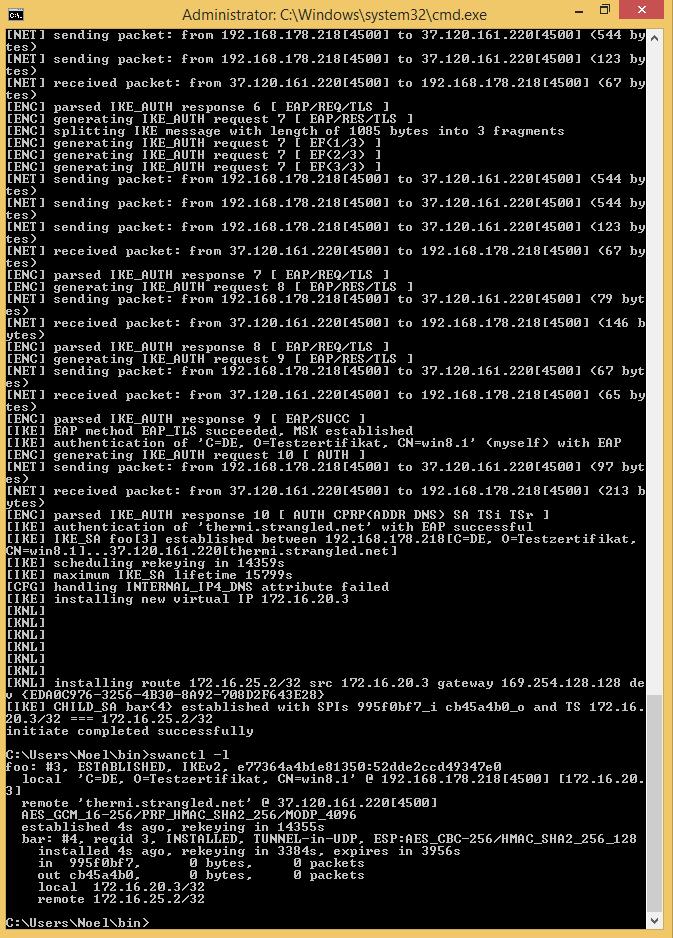
\includegraphics[width=\textwidth]{Bilder/Aufbau_und_swanctl_-l.png}
\caption{Ausgabe des Tunnelaufbaus und swanctl -l}
\label{fig:swanctl-l}
\end{figure}
\end{centering}

Die unter \autoref{lst:strongswan.conf} und \autoref{lst:swanctl.conf} bereitgestellten
Konfigurationen wurden zur Konfiguration des Dienstes genutzt.

\pagebreak

\begin{lstlisting}[caption=./configure und make]
./configure --host=x86_64-w64-mingw32 --prefix=/ --libdir=/bin --bindir=/bin --sbindir=/bin --disable-defaults --enable-monolithic --enable-static --enable-svc --enable-ikev2 
--enable-ikev1 --enable-nonce --enable-pem --enable-pkcs1 --enable-x509 --enable-openssl --enable-socket-win --enable-kernel-wfp --enable-kernel-iph --enable-pubkey --enable-swanctl 
--with-swanctldir=swanctl --with-strongswan-conf=strongswan.conf --enable-libipsec --enable-kernel-libipsec --enable-eap-tls --enable-mschapv2 --enable-eap-peap --enable-eap-gtc 
--enable-eap-dynamic --enable-eap-identity --enable-md4 --enable-ipseckey --enable-dnscert --enable-files --enable-sha3 host_alias=x86_64-w64-mingw32 CC=x86_64-w64-mingw32-gcc 
CFLAGS=-g -O2 -Wall -Werror -Wno-pointer-sign -Wno-format-security -Wno-format -mno-ms-bitfields -I/home/thermi/FH-Stuff/UNITS-8/Bachelorarbeit/win32-headers/files/include/ 
LDFLAGS=-L/home/thermi/FH-Stuff/UNITS-8/Bachelorarbeit/win32-headers/files/lib/ -L/home/thermi/FH-Stuff/UNITS-8/Bachelorarbeit/win32-headers/files/bin/
make clean && make
\end{lstlisting}


Der Befehl konfiguriert den strongSwan Quellcode zum Bauen der benötigten Plugins, sowie einiger
Extras für die Authentifizierung und dazu den 64-Bit Compiler des MINGW32-Projekts zu nutzen.

Der Code wurde getestet, indem versucht wurde eine VPN-Verbindung zu einem \ac{IKE}-Peer
unter meiner Kontrolle aufzubauen. Der ausgehandelte \ac{TS} wurde so gewählt, dass
die Beschränkung von Route based VPNs keine Rolle spielen.
Die genutzte Konfiguration ist im Appendix unter \autoref{lst:swanctl.conf}
und \autoref{lst:strongswan.conf} zu finden.

\subsection{Test der Verbindung}
Das Testen der Verbindung wurde durch durch einfaches Pingen über die Verbindung bewerkstelligt.
Dabei wird durch Dumpen der Pakete mit tcpdump und Wireshark überprüft, ob die
ARP requests auf dem TUN-Adapter beantwortet werden und ob das Paket auf dem
anderen Endpunkt auftaucht. Des weiteren werden die Traffic-Counter der \acp{SA} überprüft,
um zu überprüfen, ob die Pakete jemals verarbeitet wurden.

\subsection{Notwendige Features für Nutzung als RW auf Windows}
Um strongSwan als \ac{RW} auf Windows benutzbar zu machen werden neben dem Implementieren
der Unterstützung von TAP-Geräten unter anderem die Unterstützung der Installation von DNS-Resolvereinträgen
benötigt, da in der Regel interne DNS-Server an die \acp{RW} über Config Mode oder \acp{CP}
gesendet werden, die sie nutzen sollen.

Des weiteren wird eine Möglichkeit benötigt, um über \ac{VICI} nach Daten für dynamisch auftretende
Passwortaufforderungen, die bei der Authentifizierung mittels XAUTH oder EAP auftreten können,
zu fragen. Dies wird für die vollständige Unterstützen von \ac{MFA} benötigt.

Auf Windows benutzt das Tool ''swanctl'', welches dort zum Kontrollieren des Daemons
genutzt wird, eine TCP-Verbindung über 127.0.0.1:4502 um mit dem Daemon zu kommunizieren.
Dies ist im Vergleich zur Implementierung auf anderen Plattformen unsicher, da dort
UNIX-Sockets genutzt werden, die standardmäßig aufgrund der \acp{ACL} abgesichert werden
und nur ''root'' auf den Socket zugreifen kann. Der Wiki-Artikel macht auf die Unsicherheit
des \ac{VICI}-Protokolls, welches zwischen ''swanctl'' und ''charon'' gesprochen wird, besonders aufmerksam.
\begin{quote}
The VICI protocol runs over a reliable transport protocol. As the protocol itself currently does not provide any security or authentication properties, it is recommended to run it over a UNIX socket with appropriate permissions.
\end{quote}\cite[][]{_vici_2016}

\subsection{Probleme}
Während der \ac{BA} wurden mehrere Probleme identifiziert, die mit unbekanntem
Verhalten von Funktionen und Standards zusammenhängen.
\paragraph{C-Standard}
Eines dieser Probleme ist, dass der C-Standard die Deklaration einer Variable
direkt nach einem ''case'' eines switch-cases nur erlaubt, wenn die Deklaration
in einem Codeblock stattfindet.
Der folgende Code produziert eine Fehlermeldung:
\begin{lstlisting}[caption=Problematik mit C-Standard,label=c-standard]
void main() {
    int foo = 0;
    
    switch(foo)
    {
        case 0:
            char *bar;
            break;
        default:
            break;
    }

}
\end{lstlisting}
Die Problematik kann umgangen werden, wenn der Code im case mit geschweiften Klammern
umfasst wird, wie hier:
\begin{lstlisting}[caption=Abhilfe für Problematik mit C-Standard,label=c-standard-fix]
void main() {
    int foo = 0;
    
    switch(foo)
    {
        case 0:
        {
            char *bar;
            break;
        }
        default:
            break;
    }
}
\end{lstlisting}
\begin{filecontents*}{c-standard-error.tex}
test.c: In Funktion »main«:
test.c:7:13: Fehler: eine Marke kann nur Teil einer Anweisung sein, und eine Deklaration ist keine Anweisung
             char *bar;
             ^~~~
\end{filecontents*}

\lstinputlisting[caption=Fehlermeldung von gcc,label=c-standard-error,inputencoding=utf8/latin1]{c-standard-error.tex}

Interessanterweise ist eine Deklaration in einem ''case'' erlaubt, jedoch nur
nicht direkt nach der Deklaration des ''case''.
Daher funktioniert dieser Code auch.

\begin{lstlisting}[caption=Abhilfe mittels NOOP,label=c-standard-noop]
void main() {
    int foo = 0;
    
    switch(foo)
    {
        case 0:
            ;
            char *bar;
            break;
        default:
            break;
    }
}

\end{lstlisting}
\paragraph{WaitForSingleObject()}
Wie erläutert wird WaitForMultipleObjects() genutzt, um die IO-Operationen
zu multiplexen. Diese Funktion beendet im Programmcode mit dem Wert ''1'',
was bedeuted dass das zweite Objekt (In C werden Arrays von 0 auf indexiert.)
im Array signalisiert wurde. Bei der Überprüfung mit WaitForSingleObject() ist das jedoch nicht
der Fall. Wenn das Event signalisiert wäre, dann würde der folgende Aufruf
den Wert ''WAIT\_OBJECT\_0'' (0x0) zurückgeben:
\begin{lstlisting}
WaitForSingleObject(event_array[offset], 0)
\end{lstlisting}]
Das ist jedoch nicht der Fall. Der Aufruf beendet mit ''WAIT\_TIMEOUT'' (0x102, 258),
was bedeuted, dass das Event nicht signalisiert ist. Wenn der Rückgabewert
ignoriert wird, dann befindet sich im Puffer kein valides IPv4-Packet.

Das Problem ist besonders evident bei der Betrachtung des Debug-Logs,
welches sich auf Seite \pageref{lst:debug-log} finden lässt.
Es wird vom Code in auf Seite \pageref{lst:handle-plain-windows} ausgegeben.

\paragraph{GetLastError()}
Des weiteren gibt die Funktion ''GetLastError()'' den Fehlerwert 0 zurück, wenn sie nicht
direkt nach dem Funktionsaufruf, der den Fehlerstatus setzte, aufgerufen wird.
Es ist irrelevant, ob zwischen dem Aufruf von ''GetLastError()'' nur eine einfache Zuweisung
oder eine If-Abfrage steht.
Dies ergibt keinen Sinn, da sich der Fehlerstatus scheinbar ändert, ohne dass
eine Funktion aufgerufen wird, die das tun könnte.

% This file is part of Bachelorarbeit

% Bachelorarbeit is free software: you can redistribute it and/or modify
% it under the terms of the GNU General Public License version 3 as published by
% the Free Software Foundation.

% Bachelorarbeit is distributed in the hope that it will be useful,
% but WITHOUT ANY WARRANTY; without even the implied warranty of
% MERCHANTABILITY or FITNESS FOR A PARTICULAR PURPOSE.  See the
% GNU General Public License for more details.

% You should have received a copy of the GNU General Public License
% along with Foobar. If not, see <http://www.gnu.org/licenses/>.
\newpage

%\nocite{*}
\phantomsection
\addcontentsline{toc}{section}{Literatur}
\interlinepenalty 10000
%\bibliographystyle{alpha}
%\bibliography{bibliography}
\printbibliography
\newpage

% This file is part of Bachelorarbeit

% Bachelorarbeit is free software: you can redistribute it and/or modify
% it under the terms of the GNU General Public License version 3 as published by
% the Free Software Foundation.

% Bachelorarbeit is distributed in the hope that it will be useful,
% but WITHOUT ANY WARRANTY; without even the implied warranty of
% MERCHANTABILITY or FITNESS FOR A PARTICULAR PURPOSE.  See the
% GNU General Public License for more details.

% You should have received a copy of the GNU General Public License
% along with Foobar. If not, see <http://www.gnu.org/licenses/>.
\newpage
\section*{Eidesstattliche Erklärung}

Hiermit versichere ich eidesstattlich, dass die vorliegende Bachelor-Thesis von mir
selbstständig und ohne unerlaubte fremde Hilfe angefertigt worden ist, insbesondere,
dass ich alle Stellen, die wörtlich oder annähernd wörtlich oder dem Gedanken nach
aus Veröffentlichungen, unveröffentlichten Unterlagen und Gesprächen entnommen
worden sind, als solche an den entsprechenden Stellen innerhalb der Arbeit durch Zitate
kenntlich gemacht habe, wobei in den Zitaten jeweils der Umfang der entnommenen
Originalzitate kenntlich gemacht wurde. Ich bin mir bewusst, dass eine falsche Versicherung
rechtliche Folgen haben wird.
\vspace*{5cm}

\noindent
\begin{minipage}[h]{0.4\linewidth}
Haslach, den\dotfill\\
\vspace*{2.5mm}
\end{minipage}
\hspace*{0.1\linewidth}
\begin{minipage}[h]{0.5\linewidth}
  \begin{center}
    \dotfill\\
    Noel Kuntze
  \end{center}
\end{minipage}

% This file is part of Bachelorarbeit

% Bachelorarbeit is free software: you can redistribute it and/or modify
% it under the terms of the GNU General Public License version 3 as published by
% the Free Software Foundation.

% Bachelorarbeit is distributed in the hope that it will be useful,
% but WITHOUT ANY WARRANTY; without even the implied warranty of
% MERCHANTABILITY or FITNESS FOR A PARTICULAR PURPOSE.  See the
% GNU General Public License for more details.

% You should have received a copy of the GNU General Public License
% along with Foobar. If not, see <http://www.gnu.org/licenses/>.

\section{Appendix}
\label{sec:appendix}

\subsection{Featurematrix}
\label{subsec:featurematrix}
Die Daten aus diesen Tabellen wurden unter Nutzung der öffentlich zugänglichen
Dokumente auf den entsprechenden Herstellerwebseiten erstellt.

Wenn bei einem symmetrischen Verschlüsselungsalgorithmus kein Modus angegeben
war, wurde \ac{CBC} angenommen.

Wenn bei einem Authentifizierungsmodus nicht alle unterstützen Permutationen
angegeben waren, wurden alle standardisierten Permutationen als unterstützt 
angenommen.

Wenn ein Feature nicht explizit als unterstützt angegeben wurde, so wurde angenommen
dass es nicht unterstützt wird.

Offenbar ist der ''bintec Secure IPsec Client'' nur ein Rebranding des ''NCP Secure Entry Client'',
wenn man vom \ac{GUI} ausgehen kann. 
Ein weiteres Indiz ist, dass im Installer des ''bintec Secure IPsec Client''
der String ''NCP engineering GmbH'' auftaucht. Daher wäre es zu verstehen,
wenn aus den Dokumentationen der beiden Produkte Featureparität hervorkäme.
Dem ist aber nicht so, wie aus den Tabellen hervorgeht.

Diese Tabellen beziehen sich nur auf die Fähigkeiten, die ab Windows 7 unterstützt sind.
Sie machen keine Aussage über die Unterstützung der Software auf anderen Platformen
und hat keinen Anspruch auf Vollständigkeit.

\paragraph{Symbolik}
\begin{description}
\item[x] Unterstützt
\item[o] Nicht unterstützt
\item[?] unbekannt
\end{description}
\paragraph{Referenzen zur Bibliographie}
\begin{itemize}
\item strongSwan\footcite[][]{_ikev1ciphersuites_2016}\footcite[][]{_ikev2ciphersuites_2016}
\item Windows Agile VPN Client\footcite[][]{_windows7_2016}
\item Shrewsoft VPN Client\footcite[][]{_shrew_2013}
\item NCP Secure Entry Client\footcite[][]{jurgen_honig_datenblatt_2016}
\item bintec Secure IPsec Client\footcite[][]{_bintec_2016-1}
\end{itemize}

\begin{center}
\begin{table}[h!]
\begin{tabularx}{\textwidth}{|X|X|}\firsthline
Software & IKE-Versionen \\ \hline
strongSwan & IKEv1, IKEv2\\ \hline
Windows Agile VPN Client & IKEv1+L2TP, IKEv2 \\ \hline
Shrewsoft VPN Client & IKEv1 \\ \hline
NCP Secure Entry Client & IKEv1, IKEv2 \\ \hline
bintec Secure IPsec Client & IKEv1, IKEv2 \\ \hline
\end{tabularx}
\label{tab:IPsec-Implementierungen-IKE-Versionen}
\caption{Unterstützte IKE-Versionen der IPsec-Implementierungen}
\end{table}


\begin{table}[h!]
\begin{tabularx}{\textwidth}{|X|X|}\firsthline
Software & Lizenz \\ \hline
strongSwan & MIT/GPLv2 \\ \hline
Windows Agile VPN Client & Proprietär \\ \hline
Shrewsoft VPN Client & Shareware \\ \hline
NCP Secure Entry Client & Proprietär \\ \hline
bintec Secure IPsec Client & Proprietär \\ \hline
\end{tabularx}
\label{tab:IPsec-Implementierungen-Lizenzen}
\caption{Lizenzen der IPsec-Implementierungen}
\end{table}

\begin{table}[h!]
\begin{tabularx}{\textwidth}{|X|c|c|c|c|c|}\firsthline
\backslashbox{Modus}{Software} & strongSwan & Windows & Shrewsoft & NCP & bintec \\ \hline
AES-128-CBC          &  x  & x & x & x & x \\  \hline
AES-192-CBC          &  x  & x & x & x & x \\  \hline
AES-256-CBC          &  x  & x & x & x & x \\  \hline
AES-128-GCM-8        &  x  & o & o & o & o \\  \hline
AES-128-GCM-12       &  x  & o & o & o & o \\  \hline
AES-128-GCM-16       &  x  & o & o & o & o \\  \hline
AES-192-GCM-8        &  x  & o & o & o & o \\  \hline
AES-192-GCM-12       &  x  & o & o & o & o \\  \hline
AES-192-GCM-16       &  x  & o & o & o & o \\  \hline
AES-256-GCM-8        &  x  & o & o & o & o \\  \hline
AES-256-GCM-12       &  x  & o & o & o & o \\  \hline
AES-256-GCM-16       &  x  & o & o & o & o \\  \hline
AES-128-CTR          &  x  & o & o & o & o \\  \hline
AES-192-CTR          &  x  & o & o & o & o \\  \hline
AES-256-CTR          &  x  & o & o & o & o \\  \hline
AES-128-CCM-8        &  x  & o & o & o & o \\  \hline
AES-128-CCM-12       &  x  & o & o & o & o \\  \hline
AES-128-CCM-16       &  x  & o & o & o & o \\  \hline
AES-192-CCM-8        &  x  & o & o & o & o \\  \hline
AES-192-CCM-12       &  x  & o & o & o & o \\  \hline
AES-192-CCM-16       &  x  & o & o & o & o \\  \hline
AES-256-CCM-8        &  x  & o & o & o & o \\  \hline
AES-256-CCM-12       &  x  & o & o & o & o \\  \hline
AES-256-CCM-16       &  x  & o & o & o & o \\  \hline
DES-CBC              &  o  & o & x & o & o \\  \hline
3DES-CBC             &  x  & x & x & x & x \\  \hline
BLOWFISH-128-CBC     &  x  & o & x & x & x \\  \hline
BLOWFISH-192-CBC     &  x  & o & x & x & x \\  \hline
BLOWFISH-256-CBC     &  x  & o & x & x & x \\  \hline
CAMELLIA-128-CBC     &  x  & o & o & o & o \\  \hline
CAMELLIA-192-CBC     &  x  & o & o & o & o \\  \hline
CAMELLIA-256-CBC     &  x  & o & o & o & o \\  \hline
CAMELLIA-128-CCM-8   &  x  & o & o & o & o \\  \hline
CAMELLIA-128-CCM-12  &  x  & o & o & o & o \\  \hline
CAMELLIA-128-CCM-16  &  x  & o & o & o & o \\  \hline
CAMELLIA-192-CCM-8   &  x  & o & o & o & o \\  \hline
CAMELLIA-192-CCM-12  &  x  & o & o & o & o \\  \hline
CAMELLIA-192-CCM-16  &  x  & o & o & o & o \\  \hline
CAMELLIA-256-CCM-8   &  x  & o & o & o & o \\  \hline
CAMELLIA-256-CCM-12  &  x  & o & o & o & o \\  \hline
CAMELLIA-256-CCM-16  &  x  & o & o & o & o \\  \hline
SERPENT-128-CBC      &  x  & o & o & o & o \\  \hline
SERPENT-192-CBC      &  x  & o & o & o & o \\  \hline
SERPENT-256-CBC      &  x  & o & o & o & o \\  \hline
TWOFISH-128-CBC      &  x  & o & o & o & o \\  \hline
TWOFISH-192-CBC      &  x  & o & o & o & o \\  \hline
TWOFISH-256-CBC      &  x  & o & o & o & o \\  \hline
CAST-128-CBC         &  x  & o & x & o & o \\  \hline
chacha20poly1305     &  x  & o & o & o & o \\  \hline
\end{tabularx}
\label{tab:IPsec-Implementierungen-Vertraulichkeit-Algorithmen}
\caption{Unterstützte Algorithmen für Vertraulichkeit der IPsec-Implementierungen}
\end{table}

\begin{table}[h!]
\begin{tabularx}{\textwidth}{|X|c|c|c|c|c|}\firsthline
\backslashbox{Modus}{Software} & strongSwan & Windows & Shrewsoft & NCP & bintec \\ \hline
MD5                                                     & x & o & x & x & x \\  \hline
SHA-1                                                   & x & x & x & o & x \\  \hline
SHA-256                                                 & x & x & o & x & x \\  \hline
SHA-384                                                 & x & x & o & x & x \\  \hline
SHA-512                                                 & x & o & o & x & x \\  \hline
SHA-256-96                                              & x & x & o & o & o \\  \hline
AES-XCBC                                                & x & o & o & o & o \\  \hline
AES-128-GMAC                                            & x & o & o & o & o \\  \hline
AES-192-GMAC                                            & x & o & o & o & o \\  \hline
AES-256-GMAC                                            & x & o & o & o & o \\  \hline
\end{tabularx}
\label{tab:IPsec-Implementierungen-Authentizitaet-Algorithmen}
\caption{Unterstützte Algorithmen für Authentizität der IPsec-Implementierungen}
\end{table}

\begin{table}[h!]
\begin{tabularx}{\textwidth}{|X|c|c|c|c|c|}\firsthline
\backslashbox{Modus}{Software} & strongSwan & Windows & Shrewsoft & NCP & bintec \\ \hline
MODP-768       & x & o & x & x & x \\  \hline
MODP-1024      & x & x & x & x & x \\  \hline
MODP-1536      & x & o & x & x & x \\  \hline
MODP-2048      & x & x & x & x & x \\  \hline
MODP-3072      & x & o & x & x & x \\  \hline
MODP-4096      & x & o & x & x & x \\  \hline
MODP-6144      & x & o & x & x & x \\  \hline
MODP-8192      & x & o & x & x & x \\  \hline
MODP-1024s160  & x & o & o & o & o \\  \hline
MODP-2048s224  & x & o & o & o & o \\  \hline
MODP-2048s256  & x & o & o & o & o \\  \hline
ECP-192        & x & o & o & x & o \\  \hline
ECP-224        & x & o & o & x & o \\  \hline
ECP-256        & x & o & o & x & o \\  \hline
ECP-384        & x & o & o & x & o \\  \hline
ECP-521        & x & o & o & x & o \\  \hline
ECP-224BP      & x & o & o & o & o \\  \hline
ECP-256BP      & x & o & o & o & o \\  \hline
ECP-384BP      & x & o & o & o & o \\  \hline
ECP-512BP      & x & o & o & o & o \\  \hline
NTRU-112       & x & o & o & o & o \\  \hline
NTRU-128       & x & o & o & o & o \\  \hline
NTRU-192       & x & o & o & o & o \\  \hline
NTRU-256       & x & o & o & o & o \\  \hline
NEWHOPE-128    & x & o & o & o & o \\  \hline
\end{tabularx}
\label{tab:IPsec-Implementierungen-DH-Algorithmen}
\caption{Unterstützte Schlüsselaustauschprotokolle der IPsec-Implementierungen}
\end{table}

\begin{table}[h!]
\begin{tabularx}{\textwidth}{|X|c|c|c|c|c|}\firsthline
\backslashbox{Modus}{Software} & strongSwan & Windows & Shrewsoft & NCP & bintec                  \\ \hline
Hybrid                                                   & x & x & x & x & x  \\ \hline
PSK                                                      & x & o & x & x & o  \\ \hline
PSK + XAUTH                                              & x & o & x & x & o  \\ \hline
X.509                                                    & x & x & x & x & x  \\ \hline
EAP-MD5                                                  & x & o & o & x & o  \\ \hline
EAP-PAP                                                  & x & o & o & x & o  \\ \hline
EAP-CHAP                                                 & x & o & o & x & o  \\ \hline
EAP-MSCHAPv2                                             & x & x & o & x & o  \\ \hline
EAP-GTC                                                  & x & o & o & o & o  \\ \hline
EAP-TLS                                                  & x & x & o & x & o  \\ \hline
EAP-TTLS                                                 & x & o & o & o & o  \\ \hline
EAP-AKA                                                  & x & o & o & o & o  \\ \hline
EAP-TNC                                                  & x & o & o & o & o  \\ \hline
TNC-IMC                                                  & x & o & o & o & o  \\ \hline
TNC-IMV                                                  & x & o & o & o & o  \\ \hline
\end{tabularx}
\label{tab:IPsec-Implementierungen-Authentifizierungs-Modi}
\caption{Unterstützte Authentifizierungsmethoden der IPsec-Implementierungen}
\end{table}

\begin{table}[h!]
\begin{tabularx}{\textwidth}{|X|c|c|c|c|c|}\firsthline
\backslashbox{Modus}{Software} & strongSwan & Windows & Shrewsoft & NCP & bintec \\ \hline
CRL  & x & x & o & x & x \\ \hline
OCSP & x & ? & o & x & x \\ \hline
\end{tabularx}
\label{tab:IPsec-Implementierungen-CRL-Support}
\caption{Unterstützte Mechanismen zum Zurückziehen von Zertifikaten der IPsec-Implementierungen}
\end{table}


\begin{table}[h!]
\begin{tabularx}{\textwidth}{|X|c|c|c|c|c|}\firsthline
\backslashbox{Modus}{Software} & strongSwan & Windows & Shrewsoft & NCP & bintec \\ \hline
Tunnel-Modus     & x & x & x & x & x \\  \hline
Transport-Modus  & x & x & o & o & o \\  \hline
BEET-Modus       & x & o & o & o & o \\  \hline
\end{tabularx}
\label{tab:IPsec-Implementierungen-Tunnel-Modi}
\caption{Unterstützte Tunnel-Modi der IPsec-Implementierungen}
\end{table}

\begin{table}[h!]
\begin{tabularx}{\textwidth}{|X|c|c|c|c|c|}\firsthline
\backslashbox{Modus}{Software} & strongSwan & Windows & Shrewsoft & NCP & bintec \\ \hline
Main Mode       & x & x & x & x & ? \\ \hline
Aggressive Mode & x & x & x & x & ? \\ \hline 
Quick Mode      & x & o & x & x & ? \\ \hline
Config Mode     & x & x & x & x & x \\ \hline
\end{tabularx}
\label{tab:IPsec-Implementierungen-IKE-Modi}
\caption{Unterstützte IKE-Modi der IPsec-Implementierungen}
\end{table}

\begin{table}[h!]
\begin{tabularx}{\textwidth}{|X|c|c|c|c|c|}\firsthline
\backslashbox{Feature}{Software} & strongSwan & Windows & Shrewsoft & NCP & bintec \\ \hline
NAT-T                 & x & x                     & x & x & x \\ \hline
DPD                   & x & x                     & x & x & x \\ \hline
MOBIKE                & x & x                     & o & o & o \\ \hline
GUI                   & o & x                     & x & x & x \\ \hline
IPsec über TCP        & o & o                     & o & x & x \\ \hline
IPv6                  & x & x                     & x & x & x \\ \hline
Attribut-Zertifikate  & x & ?                     & o & o & ? \\ \hline
PFS                   & x & o                     & x & x & x \\ \hline
IKE-Fragmentierung    & x & Nur IKEv1             & x & o & o \\ \hline
Komprimierung         & x & o                     & o & x & o \\ \hline
\end{tabularx}
\label{tab:IPsec-Implementierungen-Features}
\caption{Unterstützte Features der IPsec-Implementierungen}
\end{table}
\end{center}

\subsection{Testkonfiguration}
\label{subsec:Testkonfiguration}

\begin{lstlisting}[caption=Testkonfiguration - swanctl.conf,label=lst:swanctl.conf]
connections {
        foo {
            version = 2
            dpd_delay = 10
            dpd_timeout = 60
            fragmentation = yes
            send_cert = always
            remote_addrs = 37.120.161.220
            proposals = aes256gcm16-prfsha256-modp4096
            vips = 0.0.0.0
			mobike = no
			encap = yes
            local {
                auth = eap-tls
                certs = certificate.pem
            }
            remote {
                auth = pubkey
                id = thermi.strangled.net
                cacerts = serverca.pem
            }
            children {
                    bar {
                        dpd_action = restart
                        start_action = none
                        esp_proposals = aes256-sha256-ecp521
                        remote_ts = 172.16.25.2/32
                    }
            }
        }
}
\end{lstlisting}

\begin{lstlisting}[caption=Testkonfiguration - strongswan.conf,label=lst:strongswan.conf]
charon-svc {
	filelog {
		this_log.txt{
			default=2
			job = 1
			mgr = 0
			enc = 0 
			asn = 0
			flush_line = yes
			ike_name = yes
			append = no
		}
	}
}
\end{lstlisting}

\begin{lstlisting}[caption=Code von win32.h,label=lst:libstrongswan-win32.h]
/*
 * Copyright (C) 2016 Noel Kuntze
 *
 * Permission is hereby granted, free of charge, to any person obtaining a copy
 * of this software and associated documentation files (the "Software"), to deal
 * in the Software without restriction, including without limitation the rights
 * to use, copy, modify, merge, publish, distribute, sublicense, and/or sell
 * copies of the Software, and to permit persons to whom the Software is
 * furnished to do so, subject to the following conditions:
 *
 * The above copyright notice and this permission notice shall be included in
 * all copies or substantial portions of the Software.
 *
 * THE SOFTWARE IS PROVIDED "AS IS", WITHOUT WARRANTY OF ANY KIND, EXPRESS OR
 * IMPLIED, INCLUDING BUT NOT LIMITED TO THE WARRANTIES OF MERCHANTABILITY,
 * FITNESS FOR A PARTICULAR PURPOSE AND NONINFRINGEMENT. IN NO EVENT SHALL THE
 * AUTHORS OR COPYRIGHT HOLDERS BE LIABLE FOR ANY CLAIM, DAMAGES OR OTHER
 * LIABILITY, WHETHER IN AN ACTION OF CONTRACT, TORT OR OTHERWISE, ARISING FROM,
 * OUT OF OR IN CONNECTION WITH THE SOFTWARE OR THE USE OR OTHER DEALINGS IN
 * THE SOFTWARE.
 */

#ifndef WIN32_H
#define WIN32_H

#define WIN32_TUN_READ_EVENT_TEMPLATE "WIN32-libipsec-read-device-%d"
#define WIN32_TUN_WRITE_EVENT_TEMPLATE "WIN32-libipsec-write-device-%d"
#define WIN32_TUN_EVENT_LENGTH 80
#define TAP_WIN_COMPONENT_ID "tap0901"

#define ADAPTER_KEY "SYSTEM\\CurrentControlSet\\Control\\Class\\{4D36E972-E325-11CE-BFC1-08002BE10318}"
#define NETWORK_CONNECTIONS_KEY "SYSTEM\\CurrentControlSet\\Control\\Network\\{4D36E972-E325-11CE-BFC1-08002BE10318}"

/*
 * ======================
 * Filesystem prefixes
 * ======================
 */

#define USERMODEDEVICEDIR "\\\\.\\Global\\"
#define SYSDEVICEDIR      "\\Device\\"
#define USERDEVICEDIR     "\\DosDevices\\Global\\"
#define TAP_WIN_SUFFIX    ".tap"

/*
 * TAP IOCTL constants and macros.
 *
 */
#define TAP_WIN_CONTROL_CODE(request,method) \
  CTL_CODE (FILE_DEVICE_UNKNOWN, request, method, FILE_ANY_ACCESS)

/* Present in 8.1 */

#define TAP_WIN_IOCTL_GET_MAC               TAP_WIN_CONTROL_CODE (1, METHOD_BUFFERED)
#define TAP_WIN_IOCTL_GET_VERSION           TAP_WIN_CONTROL_CODE (2, METHOD_BUFFERED)
#define TAP_WIN_IOCTL_GET_MTU               TAP_WIN_CONTROL_CODE (3, METHOD_BUFFERED)
#define TAP_WIN_IOCTL_GET_INFO              TAP_WIN_CONTROL_CODE (4, METHOD_BUFFERED)
#define TAP_WIN_IOCTL_CONFIG_POINT_TO_POINT TAP_WIN_CONTROL_CODE (5, METHOD_BUFFERED)
#define TAP_WIN_IOCTL_SET_MEDIA_STATUS      TAP_WIN_CONTROL_CODE (6, METHOD_BUFFERED)
#define TAP_WIN_IOCTL_CONFIG_DHCP_MASQ      TAP_WIN_CONTROL_CODE (7, METHOD_BUFFERED)
#define TAP_WIN_IOCTL_GET_LOG_LINE          TAP_WIN_CONTROL_CODE (8, METHOD_BUFFERED)
#define TAP_WIN_IOCTL_CONFIG_DHCP_SET_OPT   TAP_WIN_CONTROL_CODE (9, METHOD_BUFFERED)

/* Added in 8.2 */

/* obsoletes TAP_WIN_IOCTL_CONFIG_POINT_TO_POINT */
#define TAP_WIN_IOCTL_CONFIG_TUN            TAP_WIN_CONTROL_CODE (10, METHOD_BUFFERED)
#define TAP_WIN_IOCTL_CONFIG_SET_SRC_CHECK  TAP_WIN_CONTROL_CODE (11, METHOD_BUFFERED)


#endif /* WIN32_H */
\end{lstlisting}

\begin{lstlisting}[caption=Code für das Suchen eines TAP-Geräts,label=lst:find_tap_devices]
/*
 * Searches through the registry for suitable TAP driver interfaces
 * On Windows, the TAP interface metadata is stored and described in the registry.
 * It returns a linked list that contains all found guids. The guids describe the interfaces.
 */

linked_list_t *find_tap_devices()
{
    char enum_name[256], unit_string[256],
    instance_id[256], component_id[256],
    component_id_string[] = "ComponentId",
    instance_id_string[] = "NetCfgInstanceId";
    LONG status;
    uint32_t i = 0;
    DWORD len, type;
    HKEY adapter_key, unit_key;
    linked_list_t *list = linked_list_create();

    /*
     * Open parent key. It contains all other keys that
     * describe any possible interfaces.
     */
    status = RegOpenKeyEx(
            HKEY_LOCAL_MACHINE,
            ADAPTER_KEY,
            0,
            KEY_READ,
            &adapter_key);

    if (status == ERROR_SUCCESS)
    {
        while (TRUE)
        {
            len = sizeof (enum_name);
            status = RegEnumKeyEx(
                    adapter_key,
                    i,
                    enum_name,
                    &len,
                    NULL,
                    NULL,
                    NULL,
                    NULL);
            if (status == ERROR_SUCCESS)
            {
                snprintf(unit_string, sizeof (unit_string), "%s\\%s",
                        ADAPTER_KEY, enum_name);

                status = RegOpenKeyEx(
                        HKEY_LOCAL_MACHINE,
                        unit_string,
                        0,
                        KEY_READ,
                        &unit_key);

                if (status == ERROR_SUCCESS)
                {
                    len = sizeof (component_id);
                    status = RegQueryValueEx(
                            unit_key,
                            component_id_string,
                            NULL,
                            &type,
                            component_id,
                            &len);

                    if (status == ERROR_SUCCESS && type == REG_SZ)
                    {
                        len = sizeof (instance_id);
                        status = RegQueryValueEx(
                                unit_key,
                                instance_id_string,
                                NULL,
                                &type,
                                instance_id,
                                &len);

                        if (status == ERROR_SUCCESS && type == REG_SZ)
                        {
                            if (!strcmp(component_id, TAP_WIN_COMPONENT_ID))
                            {
                                /* That thing is a valid interface key */
                                /* link into return list */
                                char *guid = malloc(sizeof(instance_id));
                                memcpy(guid, instance_id, sizeof(instance_id));
                                list->insert_last(list, guid);
                            }
                        }
                    }
                    else
                    {
                        DBG2(DBG_LIB, "Error opening registry key: %s\\%s",
                                unit_string, component_id_string);
                    }
                    RegCloseKey(unit_key);
                }
                else if (status != ERROR_SUCCESS)
                {
                    DBG2(DBG_LIB, "Error opening registry key: %s", unit_string);
                }
                i++;
            }
            else if (status == ERROR_NO_MORE_ITEMS)
            {
                break;
            }
            else
            {
                DBG2(DBG_LIB, "Error enumerating registry subkeys of key: %s",
                        ADAPTER_KEY);
            }
        }
    }
    else
    {
        DBG2(DBG_LIB, "Error opening registry key: %s", ADAPTER_KEY);
    }

    RegCloseKey(adapter_key);
    return list;
}
\end{lstlisting}


\begin{lstlisting}[caption=Code für handle\_plain auf Windows,label=lst:handle-plain-windows]
/**
 * Job handling outbound plaintext packets
 */
static job_requeue_t handle_plain(private_kernel_libipsec_router_t *this)
{
#ifdef WIN32
        void **key = NULL;
        bool oldstate;
        uint32_t length, event_status = 0, i = 0, j = 0, offset;
        handle_overlapped_buffer_t *bundle_array = NULL, dummy, tun_device_handle_overlapped_buffer;
        OVERLAPPED *overlapped = NULL;
        HANDLE *event_array = NULL, tun_device_event;
        tun_device_t *tun_device = this->tun.tun;
        enumerator_t *tuns_enumerator;

        memset(&tun_device_handle_overlapped_buffer, 0, sizeof(handle_overlapped_buffer_t));
        /* Reset synchronisation event */
        ResetEvent(this->event);

        length = this->tuns->get_count(this->tuns);

        this->lock->read_lock(this->lock);
        /* Read event for this->tun */

        /* allocate arrays for all the structs we need */
        /* events, overlapped structures and bundles. */
        /* event_array holds all the HANDLE structures for the events that are
         * used for notifying the thread of finished reads and writes.
         */

        overlapped = alloca((length+2)*sizeof(OVERLAPPED));
        event_array = alloca((length+2)*sizeof(HANDLE));
        bundle_array = alloca((length+2)*sizeof(handle_overlapped_buffer_t));

        memset(overlapped, 0, (length+2)*sizeof(OVERLAPPED));
        memset(bundle_array, 0, (length+2)*sizeof(handle_overlapped_buffer_t));

        /* These are the arrays we're going to work with */

        /* first position is the event we use for synchronisation  */
        /* Insert notification event */
        event_array[i] = this->event;
        /* Insert dummy structure */
        bundle_array[i] = dummy;
        i++;

        /* second position is this->tun */
        /* insert event object for this->tun device */
        tun_device_event = CreateEvent(NULL, FALSE, FALSE, FALSE);
        if (!tun_device_event)
        {
            char *error_message = format_error(GetLastError());
            free(error_message);
            return JOB_REQUEUE_FAIR;
        }
        event_array[i] = tun_device_event;
        ResetEvent(event_array[i]);
        /* bundle for the read on this->tun */
        /* Reserve memory for the buffer*/
        tun_device_handle_overlapped_buffer.buffer = chunk_alloca(tun_device->get_mtu(tun_device));
        /* Initialise the buffer */
        memset(tun_device_handle_overlapped_buffer.buffer.ptr, 0, tun_device_handle_overlapped_buffer.buffer.len);

        tun_device_handle_overlapped_buffer.fileHandle = tun_device->get_handle(tun_device);
        tun_device_handle_overlapped_buffer.overlapped = overlapped;

        tun_device_handle_overlapped_buffer.overlapped->hEvent= tun_device_event;

        bundle_array[i] = tun_device_handle_overlapped_buffer;

        i++;

        /* Start ReadFile for this->tun.handle */
        if (!start_read(&tun_device_handle_overlapped_buffer, tun_device_handle_overlapped_buffer.overlapped->hEvent))
        {
                // TODO: Cleanup heap
                this->lock->unlock(this->lock);
                return JOB_REQUEUE_FAIR;
        }
        /* pad bundle_array with two empty structures */
        /* iterate over all our tun devices, create event handles, reset them, queue read operations on all handles */


        tuns_enumerator = this->tuns->create_enumerator(this->tuns);
        while(tuns_enumerator->enumerate(tuns_enumerator, key, &tun_device))
        {
            /* Allocate structure and buffer */

            bundle_array[i].buffer = chunk_alloca(tun_device->get_mtu(tun_device));
            memset(bundle_array[i].buffer.ptr, 0, bundle_array[i].buffer.len);
            bundle_array[i].fileHandle = tun_device->get_handle(tun_device);
            /* Allocate and initialise OVERLAPPED structure */
            bundle_array[i].overlapped = alloca(sizeof(OVERLAPPED));
            (*bundle_array[i].overlapped) = overlapped[i];
            memset(&bundle_array[i].overlapped, 0, sizeof(OVERLAPPED));
            /* Create unique name for that event. */
            /* Create unique event for read accesses on that device
             * No security attributes, no manual reset, initial state is unsignaled,
             * name is the special name we created
             */
            bundle_array[i].overlapped->hEvent = CreateEvent(NULL, FALSE, FALSE, FALSE);
            // event_array[i] = OpenEvent(EVENT_ALL_ACCESS, FALSE, tun_device->get_read_event_name(tun_device));
            event_array[i] = bundle_array[i].overlapped->hEvent;

            if (event_array[i] == NULL)
            {
                char *error_message = format_error(GetLastError());
                free(error_message);
                return JOB_REQUEUE_FAIR;
            }
            i++;

            /* Initialise read with the allocate overwrite structure */
            DBG2(DBG_ESP, "Reading on %s", tun_device->get_name(tun_device));
            if (!start_read(&bundle_array[i], bundle_array[i].overlapped->hEvent))
            {
                    // TODO: Cleanup heap
                    this->lock->unlock(this->lock);
                    return JOB_REQUEUE_FAIR;
            }
            i++;
        }
        tuns_enumerator->destroy(tuns_enumerator);

        while (TRUE)
        {
            /* Wait for a handle to be signaled */
            /* In the mingw64 sources, MAXIMUM_WAIT_OBJECTS is defined as 64. That means we can wait for a maximum of 64 event handles.
             * This translates to 63 tun devices. I think this is sufficiently high to not have to implement a mechanism for waiting for more
             * events /support more TUN devices */
            oldstate = thread_cancelability(FALSE);
            event_status = WaitForMultipleObjects(i, event_array, FALSE, INFINITE);
            thread_cancelability(oldstate);
            offset = event_status - WAIT_OBJECT_0;

            /* A handle was signaled. Find the tun handle whose read was successful */

            /* We can only use the event_status of indication for the first completed IO operation.
             * After the event was signaled, we need to test the OVERLAPPED structure in the other array
             * to find out what event was signaled.
             */
            /*
             * Probably broken?
             */
            /* Check if an event in the array was signaled. (That is the case if
             * the event_status is between WAIT_OBJECT_0 and WAIT_OBJECT_0 + nCount -1)
             */
            if ((WAIT_OBJECT_0 < event_status) && event_status < ((WAIT_OBJECT_0 + length - 1)))
            {
                /* the event at event_array[event_status - WAIT_OBJECT_0] has been signaled */
                /* It is possible that more than one event was signalled. In that case, (event_status - WAIT_OBJECT_0)
                 * is the index with the lowest event that was signalled. More signalled events can be found higher
                 *
                 * According to the documentation, WAIT_OBJECT_0 is defined as 0
                 */
                if (offset == 0)
                {
                    /* Notification about changes regarding the tun devices.
                     * Or the object is destroyed.
                     * We need to rebuild the array. So exit and rebuild. */
                    /* Cleanup
                     *  Starts with 1 to skip over the dummy
                     */
                    for(j=1;j<i;j++)
                    {
                        /* stop all asynchronous IO */
                        CancelIo(bundle_array[j].fileHandle);
                        CloseHandle(bundle_array[j].overlapped->hEvent);
                        memset(bundle_array[j].buffer.ptr, 0, bundle_array[j].buffer.len);
                        free(bundle_array[j].buffer.ptr);
                        ResetEvent(event_array[j]);
                        CloseHandle(event_array[j]);
                    }
                    /* exit */
                    return JOB_REQUEUE_DIRECT;
                }
                /* The arrays have the same length and the same positioning of the elements.
                 * Therefore, if event_array[j] is signaled, the read on bundle_array[i].fileHandle has succeeded
                 * and bundle_array[j].buffer has our data now.
                 */

                char foo[(bundle_array[offset].buffer.len *4)/3 + 1];
                memset(foo, 0, (bundle_array[offset].buffer.len *4)/3 + 1);
                chunk_to_base64(bundle_array[offset].buffer, foo);

                ip_packet_t *packet;
                /* clone the buffer */
                chunk_t buffer_clone = chunk_clone (bundle_array[offset].buffer);
                packet = ip_packet_create(buffer_clone);
                if (packet)
                {
                        ipsec->processor->queue_outbound(ipsec->processor, packet);
                }
                else
                {
                        DBG2(DBG_ESP, "invalid IP packet read from TUN device");
                }
                /* Reset the overlapped structure, event and buffer */
                /* Print out the package for debugging */
                /* Don't leak packets */
                memset(bundle_array[offset].buffer.ptr, 0, bundle_array[offset].buffer.len);
                memset(bundle_array[offset].overlapped, 0, sizeof(OVERLAPPED));

                if (!start_read(&bundle_array[offset], bundle_array[offset].overlapped->hEvent))
                {
                   /* Cleanup
                    *  Starts with 1 to skip over the dummy
                    */
                    for(j=1;j<i;j++)
                    {
                        /* stop all asynchronous IO */
                        CancelIo(bundle_array[j].fileHandle);
                        CloseHandle(bundle_array[j].overlapped->hEvent);
                        memset(bundle_array[j].buffer.ptr, 0, bundle_array[j].buffer.len);
                        free(bundle_array[j].buffer.ptr);
                    }
                    this->lock->unlock(this->lock);
                    return JOB_REQUEUE_FAIR;
                }
            }
            /* Function failed */
            else
            {
                DBG2(DBG_ESP, "waiting for events on the tun device reads failed.");

                /* Cleanup
                 *  Starts with 1 to skip over the dummy
                 */
                for(j=1;j<i;j++)
                {
                    /* stop all asynchronous IO */
                    CancelIo(bundle_array[j].fileHandle);
                    CloseHandle(bundle_array[j].overlapped->hEvent);
                    memset(bundle_array[j].buffer.ptr, 0, bundle_array[j].buffer.len);
                    free(bundle_array[j].buffer.ptr);
                    ResetEvent(event_array[j]);
                    CloseHandle(event_array[j]);
                }
                this->lock->unlock(this->lock);
                return JOB_REQUEUE_FAIR;

            }
        }
        this->lock->unlock(this->lock);
        return JOB_REQUEUE_DIRECT;
#else
        [...]
#endif /* WIN32 */
}
\end{lstlisting}

\begin{lstlisting}[caption=Debug-Log; Zeigt Problematik mit WaitForSingleObject(),label=lst:debug-log]
00[DMN] Starting IKE service charon-svc (strongSwan 5.4.1dr1, Windows Client 6.2.9200 (SP 0.0)
00[LIB] plugin 'sha3': loaded successfully
00[LIB] plugin 'md4': loaded successfully
00[LIB] plugin 'nonce': loaded successfully
00[LIB] plugin 'x509': loaded successfully
00[LIB] plugin 'pubkey': loaded successfully
00[LIB] plugin 'pkcs1': loaded successfully
00[LIB] plugin 'dnscert': loaded successfully
00[LIB] plugin 'ipseckey': loaded successfully
00[LIB] plugin 'pem': loaded successfully
00[LIB] plugin 'openssl': loaded successfully
00[LIB] plugin 'files': loaded successfully
00[LIB] Error opening registry key: SYSTEM\CurrentControlSet\Control\Class\{4D36E972-E325-11CE-BFC1-08002BE10318}\Properties
00[LIB] TAP-Windows driver version 9.22 available.
00[LIB] created TUN device: {EDA0C976-3256-4B30-8A92-708D2F643E28}
00[LIB] plugin 'kernel-libipsec': loaded successfully
00[LIB] plugin 'kernel-wfp': loaded successfully
00[LIB] plugin 'kernel-iph': loaded successfully
00[LIB] plugin 'socket-win': loaded successfully
00[LIB] plugin 'vici': loaded successfully
00[LIB] plugin 'eap-identity': loaded successfully
00[LIB] plugin 'eap-gtc': loaded successfully
00[LIB] plugin 'eap-dynamic': loaded successfully
00[LIB] plugin 'eap-tls': loaded successfully
00[LIB] plugin 'eap-peap': loaded successfully
00[LIB] feature CUSTOM:kernel-ipsec in plugin 'kernel-wfp' failed to load
00[LIB] feature PUBKEY:DSA in plugin 'pem' has unmet dependency: PUBKEY:DSA
00[LIB] feature CUSTOM:dnscert in plugin 'dnscert' has unmet dependency: RESOLVER
00[LIB] feature CUSTOM:ipseckey in plugin 'ipseckey' has unmet dependency: RESOLVER
00[LIB] feature PRIVKEY:DSA in plugin 'pem' has unmet dependency: PRIVKEY:DSA
00[LIB] feature PRIVKEY:BLISS in plugin 'pem' has unmet dependency: PRIVKEY:BLISS
00[LIB] feature CERT_DECODE:PGP in plugin 'pem' has unmet dependency: CERT_DECODE:PGP
00[LIB] feature CERT_DECODE:OCSP_REQUEST in plugin 'pem' has unmet dependency: CERT_DECODE:OCSP_REQUEST
00[LIB] unloading plugin 'dnscert' without loaded features
00[LIB] unloading plugin 'ipseckey' without loaded features
00[LIB] unloading plugin 'kernel-wfp' without loaded features
00[LIB] loaded plugins: charon-svc sha3 md4 nonce x509 pubkey pkcs1 pem openssl files kernel-libipsec kernel-iph socket-win vici eap-identity eap-gtc eap-dynamic eap-tls eap-peap
00[LIB] unable to load 8 plugin features (7 due to unmet dependencies)
00[JOB] spawning 16 worker threads
00[LIB] created thread 4016
00[LIB] created thread 3032
00[LIB] created thread 3216
00[LIB] created thread 3876
00[LIB] created thread 3132
00[LIB] created thread 1580
00[LIB] created thread 1244
00[LIB] created thread 4212
00[LIB] created thread 3152
00[LIB] created thread 4208
00[LIB] created thread 2560
00[LIB] created thread 2764
00[LIB] created thread 1604
00[LIB] created thread 4220
00[LIB] created thread 1304
00[LIB] created thread 972
08[ESP] entered handle_plain.
08[ESP] Allocated arrays, opened events
08[ESP] put notification event into index 0
08[ESP] Put TUN {EDA0C976-3256-4B30-8A92-708D2F643E28} event in index 1
08[ESP] Allocated buffer.
08[ESP] Allocated file handle.
08[ESP] Allocated overlapped..
08[ESP] Created event
08[ESP] ReadFile() returned 0
08[ESP] Error 997
08[ESP] Read on tun device is pending.
08[ESP] Enumerating tun devices ...
08[ESP] Waiting for events...
08[ESP] Event triggered with event_status 1
08[ESP] offset == 1
08[ESP] position 1 in array
08[ESP] checking if event is signaled.
08[ESP] WaitForSingleObject returned 258
08[ESP] Event is not signaled.
08[ESP] Waiting for events...
[...]
\end{lstlisting}

\begin{lstlisting}[caption=Ausgabe von ipconfig und route -4 print,label=lst:ipconfigroute4]
C:\Users\Noel\bin>ipconfig

Windows-IP-Konfiguration


Ethernet-Adapter THIS IS A TAP DEVICE:

   Verbindungsspezifisches DNS-Suffix:
   Verbindungslokale IPv6-Adresse  . : fe80::596b:bf92:963f:63a3%8
   IPv4-Adresse  . . . . . . . . . . : 172.16.20.2
   Subnetzmaske  . . . . . . . . . . : 255.255.255.255
   Standardgateway . . . . . . . . . :

Ethernet-Adapter Ethernet:

   Verbindungsspezifisches DNS-Suffix: thermicorp.lan
   IPv6-Adresse. . . . . . . . . . . : 2a02:8071:9282:e600:3031:9c6b:6485:3cc9
   Temporäre IPv6-Adresse. . . . . . : 2a02:8071:9282:e600:5181:db51:f4d7:2afa
   Temporäre IPv6-Adresse. . . . . . : 2a02:8071:9282:e600:7154:ac74:30c4:cbee
   Verbindungslokale IPv6-Adresse  . : fe80::3031:9c6b:6485:3cc9%3
   IPv4-Adresse  . . . . . . . . . . : 192.168.178.218
   Subnetzmaske  . . . . . . . . . . : 255.255.255.0
   Standardgateway . . . . . . . . . : fe80::a96:d7ff:fe85:e002%3
                                       192.168.178.1

Tunneladapter isatap.{EDA0C976-3256-4B30-8A92-708D2F643E28}:

   Medienstatus. . . . . . . . . . . : Medium getrennt
   Verbindungsspezifisches DNS-Suffix:

Tunneladapter Teredo Tunneling Pseudo-Interface:

   Medienstatus. . . . . . . . . . . : Medium getrennt
   Verbindungsspezifisches DNS-Suffix:

Tunneladapter isatap.thermicorp.lan:

   Medienstatus. . . . . . . . . . . : Medium getrennt
   Verbindungsspezifisches DNS-Suffix: thermicorp.lan


C:\Users\Noel\bin>route -4 print
===========================================================================
Schnittstellenliste
  8...00 ff ed a0 c9 76 ......TAP-Windows Adapter V9
  3...08 00 27 ef 0b 0e ......Intel(R) PRO/1000 MT-Desktopadapter
  1...........................Software Loopback Interface 1
  4...00 00 00 00 00 00 00 e0 Microsoft-ISATAP-Adapter
  5...00 00 00 00 00 00 00 e0 Teredo Tunneling Pseudo-Interface
  6...00 00 00 00 00 00 00 e0 Microsoft-ISATAP-Adapter #2
===========================================================================

IPv4-Routentabelle
===========================================================================
Aktive Routen:
     Netzwerkziel    Netzwerkmaske          Gateway    Schnittstelle Metrik
          0.0.0.0          0.0.0.0    192.168.178.1  192.168.178.218     10
        127.0.0.0        255.0.0.0   Auf Verbindung         127.0.0.1    306
        127.0.0.1  255.255.255.255   Auf Verbindung         127.0.0.1    306
  127.255.255.255  255.255.255.255   Auf Verbindung         127.0.0.1    306
      172.16.20.2  255.255.255.255   Auf Verbindung       172.16.20.2    276
      172.16.25.2  255.255.255.255  169.254.128.128      172.16.20.2     30
    192.168.178.0    255.255.255.0   Auf Verbindung   192.168.178.218    266
  192.168.178.218  255.255.255.255   Auf Verbindung   192.168.178.218    266
  192.168.178.255  255.255.255.255   Auf Verbindung   192.168.178.218    266
        224.0.0.0        240.0.0.0   Auf Verbindung         127.0.0.1    306
        224.0.0.0        240.0.0.0   Auf Verbindung       172.16.20.2    276
        224.0.0.0        240.0.0.0   Auf Verbindung   192.168.178.218    266
  255.255.255.255  255.255.255.255   Auf Verbindung         127.0.0.1    306
  255.255.255.255  255.255.255.255   Auf Verbindung       172.16.20.2    276
  255.255.255.255  255.255.255.255   Auf Verbindung   192.168.178.218    266
===========================================================================
Ständige Routen:
  Keine

\end{lstlisting}
\subsection{Lizensierung der Arbeit}
Diese \ac{BA} steht unter der GNU General Public License Version 3 (GPLv3)
und darf unter Berücksichtigung der Lizensvereinbarung der GPLv3 verfielfältigt
und verteilt werden. Der Lizenztext ist in~\autoref{subsec:gplv3} oder 
auf der offiziellen Webseite\footnote{\url{https://www.gnu.org/licenses/gpl.html}}
zu finden.

Das Logo der \ac{HSO} steht unter seiner eigenen Lizenz. Es steht nicht unter der GPLv3.
Der gesamte Code steht unter der URL \url{https://github.com/Thermi/Bachelorarbeit} zur Verfügung.

\begin{centering} 

Diese Arbeit wurde mittels \LaTeX{} erstellt
\end{centering}

\subsection{Lizenz}
\label{subsec:gplv3}
\title{GNU GENERAL PUBLIC LICENSE}
\date{Version 3, 29 June 2007}

\maketitle

\begin{center}
{\parindent 0in

Copyright \copyright\  2007 Free Software Foundation, Inc. \texttt{http://fsf.org/}

\bigskip
Everyone is permitted to copy and distribute verbatim copies of this

license document, but changing it is not allowed.}

\end{center}

\renewcommand{\abstractname}{Preamble}
\begin{abstract}
The GNU General Public License is a free, copyleft license for
software and other kinds of works.

The licenses for most software and other practical works are designed
to take away your freedom to share and change the works.  By contrast,
the GNU General Public License is intended to guarantee your freedom to
share and change all versions of a program--to make sure it remains free
software for all its users.  We, the Free Software Foundation, use the
GNU General Public License for most of our software; it applies also to
any other work released this way by its authors.  You can apply it to
your programs, too.

When we speak of free software, we are referring to freedom, not
price.  Our General Public Licenses are designed to make sure that you
have the freedom to distribute copies of free software (and charge for
them if you wish), that you receive source code or can get it if you
want it, that you can change the software or use pieces of it in new
free programs, and that you know you can do these things.

To protect your rights, we need to prevent others from denying you
these rights or asking you to surrender the rights.  Therefore, you have
certain responsibilities if you distribute copies of the software, or if
you modify it: responsibilities to respect the freedom of others.

For example, if you distribute copies of such a program, whether
gratis or for a fee, you must pass on to the recipients the same
freedoms that you received.  You must make sure that they, too, receive
or can get the source code.  And you must show them these terms so they
know their rights.

Developers that use the GNU GPL protect your rights with two steps:
(1) assert copyright on the software, and (2) offer you this License
giving you legal permission to copy, distribute and/or modify it.

For the developers' and authors' protection, the GPL clearly explains
that there is no warranty for this free software.  For both users' and
authors' sake, the GPL requires that modified versions be marked as
changed, so that their problems will not be attributed erroneously to
authors of previous versions.

Some devices are designed to deny users access to install or run
modified versions of the software inside them, although the manufacturer
can do so.  This is fundamentally incompatible with the aim of
protecting users' freedom to change the software.  The systematic
pattern of such abuse occurs in the area of products for individuals to
use, which is precisely where it is most unacceptable.  Therefore, we
have designed this version of the GPL to prohibit the practice for those
products.  If such problems arise substantially in other domains, we
stand ready to extend this provision to those domains in future versions
of the GPL, as needed to protect the freedom of users.

Finally, every program is threatened constantly by software patents.
States should not allow patents to restrict development and use of
software on general-purpose computers, but in those that do, we wish to
avoid the special danger that patents applied to a free program could
make it effectively proprietary.  To prevent this, the GPL assures that
patents cannot be used to render the program non-free.

The precise terms and conditions for copying, distribution and
modification follow.
\end{abstract}

\begin{center}
{\Large \sc Terms and Conditions}
\end{center}


\begin{enumerate}

\addtocounter{enumi}{-1}

\item Definitions.

``This License'' refers to version 3 of the GNU General Public License.

``Copyright'' also means copyright-like laws that apply to other kinds of
works, such as semiconductor masks.

``The Program'' refers to any copyrightable work licensed under this
License.  Each licensee is addressed as ``you''.  ``Licensees'' and
``recipients'' may be individuals or organizations.

To ``modify'' a work means to copy from or adapt all or part of the work
in a fashion requiring copyright permission, other than the making of an
exact copy.  The resulting work is called a ``modified version'' of the
earlier work or a work ``based on'' the earlier work.

A ``covered work'' means either the unmodified Program or a work based
on the Program.

To ``propagate'' a work means to do anything with it that, without
permission, would make you directly or secondarily liable for
infringement under applicable copyright law, except executing it on a
computer or modifying a private copy.  Propagation includes copying,
distribution (with or without modification), making available to the
public, and in some countries other activities as well.

To ``convey'' a work means any kind of propagation that enables other
parties to make or receive copies.  Mere interaction with a user through
a computer network, with no transfer of a copy, is not conveying.

An interactive user interface displays ``Appropriate Legal Notices''
to the extent that it includes a convenient and prominently visible
feature that (1) displays an appropriate copyright notice, and (2)
tells the user that there is no warranty for the work (except to the
extent that warranties are provided), that licensees may convey the
work under this License, and how to view a copy of this License.  If
the interface presents a list of user commands or options, such as a
menu, a prominent item in the list meets this criterion.

\item Source Code.

The ``source code'' for a work means the preferred form of the work
for making modifications to it.  ``Object code'' means any non-source
form of a work.

A ``Standard Interface'' means an interface that either is an official
standard defined by a recognized standards body, or, in the case of
interfaces specified for a particular programming language, one that
is widely used among developers working in that language.

The ``System Libraries'' of an executable work include anything, other
than the work as a whole, that (a) is included in the normal form of
packaging a Major Component, but which is not part of that Major
Component, and (b) serves only to enable use of the work with that
Major Component, or to implement a Standard Interface for which an
implementation is available to the public in source code form.  A
``Major Component'', in this context, means a major essential component
(kernel, window system, and so on) of the specific operating system
(if any) on which the executable work runs, or a compiler used to
produce the work, or an object code interpreter used to run it.

The ``Corresponding Source'' for a work in object code form means all
the source code needed to generate, install, and (for an executable
work) run the object code and to modify the work, including scripts to
control those activities.  However, it does not include the work's
System Libraries, or general-purpose tools or generally available free
programs which are used unmodified in performing those activities but
which are not part of the work.  For example, Corresponding Source
includes interface definition files associated with source files for
the work, and the source code for shared libraries and dynamically
linked subprograms that the work is specifically designed to require,
such as by intimate data communication or control flow between those
subprograms and other parts of the work.

The Corresponding Source need not include anything that users
can regenerate automatically from other parts of the Corresponding
Source.

The Corresponding Source for a work in source code form is that
same work.

\item Basic Permissions.

All rights granted under this License are granted for the term of
copyright on the Program, and are irrevocable provided the stated
conditions are met.  This License explicitly affirms your unlimited
permission to run the unmodified Program.  The output from running a
covered work is covered by this License only if the output, given its
content, constitutes a covered work.  This License acknowledges your
rights of fair use or other equivalent, as provided by copyright law.

You may make, run and propagate covered works that you do not
convey, without conditions so long as your license otherwise remains
in force.  You may convey covered works to others for the sole purpose
of having them make modifications exclusively for you, or provide you
with facilities for running those works, provided that you comply with
the terms of this License in conveying all material for which you do
not control copyright.  Those thus making or running the covered works
for you must do so exclusively on your behalf, under your direction
and control, on terms that prohibit them from making any copies of
your copyrighted material outside their relationship with you.

Conveying under any other circumstances is permitted solely under
the conditions stated below.  Sublicensing is not allowed; section 10
makes it unnecessary.

\item Protecting Users' Legal Rights From Anti-Circumvention Law.

No covered work shall be deemed part of an effective technological
measure under any applicable law fulfilling obligations under article
11 of the WIPO copyright treaty adopted on 20 December 1996, or
similar laws prohibiting or restricting circumvention of such
measures.

When you convey a covered work, you waive any legal power to forbid
circumvention of technological measures to the extent such circumvention
is effected by exercising rights under this License with respect to
the covered work, and you disclaim any intention to limit operation or
modification of the work as a means of enforcing, against the work's
users, your or third parties' legal rights to forbid circumvention of
technological measures.

\item Conveying Verbatim Copies.

You may convey verbatim copies of the Program's source code as you
receive it, in any medium, provided that you conspicuously and
appropriately publish on each copy an appropriate copyright notice;
keep intact all notices stating that this License and any
non-permissive terms added in accord with section 7 apply to the code;
keep intact all notices of the absence of any warranty; and give all
recipients a copy of this License along with the Program.

You may charge any price or no price for each copy that you convey,
and you may offer support or warranty protection for a fee.

\item Conveying Modified Source Versions.

You may convey a work based on the Program, or the modifications to
produce it from the Program, in the form of source code under the
terms of section 4, provided that you also meet all of these conditions:
  \begin{enumerate}
  \item The work must carry prominent notices stating that you modified
  it, and giving a relevant date.

  \item The work must carry prominent notices stating that it is
  released under this License and any conditions added under section
  7.  This requirement modifies the requirement in section 4 to
  ``keep intact all notices''.

  \item You must license the entire work, as a whole, under this
  License to anyone who comes into possession of a copy.  This
  License will therefore apply, along with any applicable section 7
  additional terms, to the whole of the work, and all its parts,
  regardless of how they are packaged.  This License gives no
  permission to license the work in any other way, but it does not
  invalidate such permission if you have separately received it.

  \item If the work has interactive user interfaces, each must display
  Appropriate Legal Notices; however, if the Program has interactive
  interfaces that do not display Appropriate Legal Notices, your
  work need not make them do so.
\end{enumerate}
A compilation of a covered work with other separate and independent
works, which are not by their nature extensions of the covered work,
and which are not combined with it such as to form a larger program,
in or on a volume of a storage or distribution medium, is called an
``aggregate'' if the compilation and its resulting copyright are not
used to limit the access or legal rights of the compilation's users
beyond what the individual works permit.  Inclusion of a covered work
in an aggregate does not cause this License to apply to the other
parts of the aggregate.

\item Conveying Non-Source Forms.

You may convey a covered work in object code form under the terms
of sections 4 and 5, provided that you also convey the
machine-readable Corresponding Source under the terms of this License,
in one of these ways:
  \begin{enumerate}
  \item Convey the object code in, or embodied in, a physical product
  (including a physical distribution medium), accompanied by the
  Corresponding Source fixed on a durable physical medium
  customarily used for software interchange.

  \item Convey the object code in, or embodied in, a physical product
  (including a physical distribution medium), accompanied by a
  written offer, valid for at least three years and valid for as
  long as you offer spare parts or customer support for that product
  model, to give anyone who possesses the object code either (1) a
  copy of the Corresponding Source for all the software in the
  product that is covered by this License, on a durable physical
  medium customarily used for software interchange, for a price no
  more than your reasonable cost of physically performing this
  conveying of source, or (2) access to copy the
  Corresponding Source from a network server at no charge.

  \item Convey individual copies of the object code with a copy of the
  written offer to provide the Corresponding Source.  This
  alternative is allowed only occasionally and noncommercially, and
  only if you received the object code with such an offer, in accord
  with subsection 6b.

  \item Convey the object code by offering access from a designated
  place (gratis or for a charge), and offer equivalent access to the
  Corresponding Source in the same way through the same place at no
  further charge.  You need not require recipients to copy the
  Corresponding Source along with the object code.  If the place to
  copy the object code is a network server, the Corresponding Source
  may be on a different server (operated by you or a third party)
  that supports equivalent copying facilities, provided you maintain
  clear directions next to the object code saying where to find the
  Corresponding Source.  Regardless of what server hosts the
  Corresponding Source, you remain obligated to ensure that it is
  available for as long as needed to satisfy these requirements.

  \item Convey the object code using peer-to-peer transmission, provided
  you inform other peers where the object code and Corresponding
  Source of the work are being offered to the general public at no
  charge under subsection 6d.
  \end{enumerate}

A separable portion of the object code, whose source code is excluded
from the Corresponding Source as a System Library, need not be
included in conveying the object code work.

A ``User Product'' is either (1) a ``consumer product'', which means any
tangible personal property which is normally used for personal, family,
or household purposes, or (2) anything designed or sold for incorporation
into a dwelling.  In determining whether a product is a consumer product,
doubtful cases shall be resolved in favor of coverage.  For a particular
product received by a particular user, ``normally used'' refers to a
typical or common use of that class of product, regardless of the status
of the particular user or of the way in which the particular user
actually uses, or expects or is expected to use, the product.  A product
is a consumer product regardless of whether the product has substantial
commercial, industrial or non-consumer uses, unless such uses represent
the only significant mode of use of the product.

``Installation Information'' for a User Product means any methods,
procedures, authorization keys, or other information required to install
and execute modified versions of a covered work in that User Product from
a modified version of its Corresponding Source.  The information must
suffice to ensure that the continued functioning of the modified object
code is in no case prevented or interfered with solely because
modification has been made.

If you convey an object code work under this section in, or with, or
specifically for use in, a User Product, and the conveying occurs as
part of a transaction in which the right of possession and use of the
User Product is transferred to the recipient in perpetuity or for a
fixed term (regardless of how the transaction is characterized), the
Corresponding Source conveyed under this section must be accompanied
by the Installation Information.  But this requirement does not apply
if neither you nor any third party retains the ability to install
modified object code on the User Product (for example, the work has
been installed in ROM).

The requirement to provide Installation Information does not include a
requirement to continue to provide support service, warranty, or updates
for a work that has been modified or installed by the recipient, or for
the User Product in which it has been modified or installed.  Access to a
network may be denied when the modification itself materially and
adversely affects the operation of the network or violates the rules and
protocols for communication across the network.

Corresponding Source conveyed, and Installation Information provided,
in accord with this section must be in a format that is publicly
documented (and with an implementation available to the public in
source code form), and must require no special password or key for
unpacking, reading or copying.

\item Additional Terms.

``Additional permissions'' are terms that supplement the terms of this
License by making exceptions from one or more of its conditions.
Additional permissions that are applicable to the entire Program shall
be treated as though they were included in this License, to the extent
that they are valid under applicable law.  If additional permissions
apply only to part of the Program, that part may be used separately
under those permissions, but the entire Program remains governed by
this License without regard to the additional permissions.

When you convey a copy of a covered work, you may at your option
remove any additional permissions from that copy, or from any part of
it.  (Additional permissions may be written to require their own
removal in certain cases when you modify the work.)  You may place
additional permissions on material, added by you to a covered work,
for which you have or can give appropriate copyright permission.

Notwithstanding any other provision of this License, for material you
add to a covered work, you may (if authorized by the copyright holders of
that material) supplement the terms of this License with terms:
  \begin{enumerate}
  \item Disclaiming warranty or limiting liability differently from the
  terms of sections 15 and 16 of this License; or

  \item Requiring preservation of specified reasonable legal notices or
  author attributions in that material or in the Appropriate Legal
  Notices displayed by works containing it; or

  \item Prohibiting misrepresentation of the origin of that material, or
  requiring that modified versions of such material be marked in
  reasonable ways as different from the original version; or

  \item Limiting the use for publicity purposes of names of licensors or
  authors of the material; or

  \item Declining to grant rights under trademark law for use of some
  trade names, trademarks, or service marks; or

  \item Requiring indemnification of licensors and authors of that
  material by anyone who conveys the material (or modified versions of
  it) with contractual assumptions of liability to the recipient, for
  any liability that these contractual assumptions directly impose on
  those licensors and authors.
  \end{enumerate}

All other non-permissive additional terms are considered ``further
restrictions'' within the meaning of section 10.  If the Program as you
received it, or any part of it, contains a notice stating that it is
governed by this License along with a term that is a further
restriction, you may remove that term.  If a license document contains
a further restriction but permits relicensing or conveying under this
License, you may add to a covered work material governed by the terms
of that license document, provided that the further restriction does
not survive such relicensing or conveying.

If you add terms to a covered work in accord with this section, you
must place, in the relevant source files, a statement of the
additional terms that apply to those files, or a notice indicating
where to find the applicable terms.

Additional terms, permissive or non-permissive, may be stated in the
form of a separately written license, or stated as exceptions;
the above requirements apply either way.

\item Termination.

You may not propagate or modify a covered work except as expressly
provided under this License.  Any attempt otherwise to propagate or
modify it is void, and will automatically terminate your rights under
this License (including any patent licenses granted under the third
paragraph of section 11).

However, if you cease all violation of this License, then your
license from a particular copyright holder is reinstated (a)
provisionally, unless and until the copyright holder explicitly and
finally terminates your license, and (b) permanently, if the copyright
holder fails to notify you of the violation by some reasonable means
prior to 60 days after the cessation.

Moreover, your license from a particular copyright holder is
reinstated permanently if the copyright holder notifies you of the
violation by some reasonable means, this is the first time you have
received notice of violation of this License (for any work) from that
copyright holder, and you cure the violation prior to 30 days after
your receipt of the notice.

Termination of your rights under this section does not terminate the
licenses of parties who have received copies or rights from you under
this License.  If your rights have been terminated and not permanently
reinstated, you do not qualify to receive new licenses for the same
material under section 10.

\item Acceptance Not Required for Having Copies.

You are not required to accept this License in order to receive or
run a copy of the Program.  Ancillary propagation of a covered work
occurring solely as a consequence of using peer-to-peer transmission
to receive a copy likewise does not require acceptance.  However,
nothing other than this License grants you permission to propagate or
modify any covered work.  These actions infringe copyright if you do
not accept this License.  Therefore, by modifying or propagating a
covered work, you indicate your acceptance of this License to do so.

\item Automatic Licensing of Downstream Recipients.

Each time you convey a covered work, the recipient automatically
receives a license from the original licensors, to run, modify and
propagate that work, subject to this License.  You are not responsible
for enforcing compliance by third parties with this License.

An ``entity transaction'' is a transaction transferring control of an
organization, or substantially all assets of one, or subdividing an
organization, or merging organizations.  If propagation of a covered
work results from an entity transaction, each party to that
transaction who receives a copy of the work also receives whatever
licenses to the work the party's predecessor in interest had or could
give under the previous paragraph, plus a right to possession of the
Corresponding Source of the work from the predecessor in interest, if
the predecessor has it or can get it with reasonable efforts.

You may not impose any further restrictions on the exercise of the
rights granted or affirmed under this License.  For example, you may
not impose a license fee, royalty, or other charge for exercise of
rights granted under this License, and you may not initiate litigation
(including a cross-claim or counterclaim in a lawsuit) alleging that
any patent claim is infringed by making, using, selling, offering for
sale, or importing the Program or any portion of it.

\item Patents.

A ``contributor'' is a copyright holder who authorizes use under this
License of the Program or a work on which the Program is based.  The
work thus licensed is called the contributor's ``contributor version''.

A contributor's ``essential patent claims'' are all patent claims
owned or controlled by the contributor, whether already acquired or
hereafter acquired, that would be infringed by some manner, permitted
by this License, of making, using, or selling its contributor version,
but do not include claims that would be infringed only as a
consequence of further modification of the contributor version.  For
purposes of this definition, ``control'' includes the right to grant
patent sublicenses in a manner consistent with the requirements of
this License.

Each contributor grants you a non-exclusive, worldwide, royalty-free
patent license under the contributor's essential patent claims, to
make, use, sell, offer for sale, import and otherwise run, modify and
propagate the contents of its contributor version.

In the following three paragraphs, a ``patent license'' is any express
agreement or commitment, however denominated, not to enforce a patent
(such as an express permission to practice a patent or covenant not to
sue for patent infringement).  To ``grant'' such a patent license to a
party means to make such an agreement or commitment not to enforce a
patent against the party.

If you convey a covered work, knowingly relying on a patent license,
and the Corresponding Source of the work is not available for anyone
to copy, free of charge and under the terms of this License, through a
publicly available network server or other readily accessible means,
then you must either (1) cause the Corresponding Source to be so
available, or (2) arrange to deprive yourself of the benefit of the
patent license for this particular work, or (3) arrange, in a manner
consistent with the requirements of this License, to extend the patent
license to downstream recipients.  ``Knowingly relying'' means you have
actual knowledge that, but for the patent license, your conveying the
covered work in a country, or your recipient's use of the covered work
in a country, would infringe one or more identifiable patents in that
country that you have reason to believe are valid.

If, pursuant to or in connection with a single transaction or
arrangement, you convey, or propagate by procuring conveyance of, a
covered work, and grant a patent license to some of the parties
receiving the covered work authorizing them to use, propagate, modify
or convey a specific copy of the covered work, then the patent license
you grant is automatically extended to all recipients of the covered
work and works based on it.

A patent license is ``discriminatory'' if it does not include within
the scope of its coverage, prohibits the exercise of, or is
conditioned on the non-exercise of one or more of the rights that are
specifically granted under this License.  You may not convey a covered
work if you are a party to an arrangement with a third party that is
in the business of distributing software, under which you make payment
to the third party based on the extent of your activity of conveying
the work, and under which the third party grants, to any of the
parties who would receive the covered work from you, a discriminatory
patent license (a) in connection with copies of the covered work
conveyed by you (or copies made from those copies), or (b) primarily
for and in connection with specific products or compilations that
contain the covered work, unless you entered into that arrangement,
or that patent license was granted, prior to 28 March 2007.

Nothing in this License shall be construed as excluding or limiting
any implied license or other defenses to infringement that may
otherwise be available to you under applicable patent law.

\item No Surrender of Others' Freedom.

If conditions are imposed on you (whether by court order, agreement or
otherwise) that contradict the conditions of this License, they do not
excuse you from the conditions of this License.  If you cannot convey a
covered work so as to satisfy simultaneously your obligations under this
License and any other pertinent obligations, then as a consequence you may
not convey it at all.  For example, if you agree to terms that obligate you
to collect a royalty for further conveying from those to whom you convey
the Program, the only way you could satisfy both those terms and this
License would be to refrain entirely from conveying the Program.

\item Use with the GNU Affero General Public License.

Notwithstanding any other provision of this License, you have
permission to link or combine any covered work with a work licensed
under version 3 of the GNU Affero General Public License into a single
combined work, and to convey the resulting work.  The terms of this
License will continue to apply to the part which is the covered work,
but the special requirements of the GNU Affero General Public License,
section 13, concerning interaction through a network will apply to the
combination as such.

\item Revised Versions of this License.

The Free Software Foundation may publish revised and/or new versions of
the GNU General Public License from time to time.  Such new versions will
be similar in spirit to the present version, but may differ in detail to
address new problems or concerns.

Each version is given a distinguishing version number.  If the
Program specifies that a certain numbered version of the GNU General
Public License ``or any later version'' applies to it, you have the
option of following the terms and conditions either of that numbered
version or of any later version published by the Free Software
Foundation.  If the Program does not specify a version number of the
GNU General Public License, you may choose any version ever published
by the Free Software Foundation.

If the Program specifies that a proxy can decide which future
versions of the GNU General Public License can be used, that proxy's
public statement of acceptance of a version permanently authorizes you
to choose that version for the Program.

Later license versions may give you additional or different
permissions.  However, no additional obligations are imposed on any
author or copyright holder as a result of your choosing to follow a
later version.

\item Disclaimer of Warranty.

\begin{sloppypar}
 THERE IS NO WARRANTY FOR THE PROGRAM, TO THE EXTENT PERMITTED BY
 APPLICABLE LAW.  EXCEPT WHEN OTHERWISE STATED IN WRITING THE
 COPYRIGHT HOLDERS AND/OR OTHER PARTIES PROVIDE THE PROGRAM ``AS IS''
 WITHOUT WARRANTY OF ANY KIND, EITHER EXPRESSED OR IMPLIED,
 INCLUDING, BUT NOT LIMITED TO, THE IMPLIED WARRANTIES OF
 MERCHANTABILITY AND FITNESS FOR A PARTICULAR PURPOSE.  THE ENTIRE
 RISK AS TO THE QUALITY AND PERFORMANCE OF THE PROGRAM IS WITH YOU.
 SHOULD THE PROGRAM PROVE DEFECTIVE, YOU ASSUME THE COST OF ALL
 NECESSARY SERVICING, REPAIR OR CORRECTION.
\end{sloppypar}

\item Limitation of Liability.

 IN NO EVENT UNLESS REQUIRED BY APPLICABLE LAW OR AGREED TO IN
 WRITING WILL ANY COPYRIGHT HOLDER, OR ANY OTHER PARTY WHO MODIFIES
 AND/OR CONVEYS THE PROGRAM AS PERMITTED ABOVE, BE LIABLE TO YOU FOR
 DAMAGES, INCLUDING ANY GENERAL, SPECIAL, INCIDENTAL OR CONSEQUENTIAL
 DAMAGES ARISING OUT OF THE USE OR INABILITY TO USE THE PROGRAM
 (INCLUDING BUT NOT LIMITED TO LOSS OF DATA OR DATA BEING RENDERED
 INACCURATE OR LOSSES SUSTAINED BY YOU OR THIRD PARTIES OR A FAILURE
 OF THE PROGRAM TO OPERATE WITH ANY OTHER PROGRAMS), EVEN IF SUCH
 HOLDER OR OTHER PARTY HAS BEEN ADVISED OF THE POSSIBILITY OF SUCH
 DAMAGES.

\item Interpretation of Sections 15 and 16.

If the disclaimer of warranty and limitation of liability provided
above cannot be given local legal effect according to their terms,
reviewing courts shall apply local law that most closely approximates
an absolute waiver of all civil liability in connection with the
Program, unless a warranty or assumption of liability accompanies a
copy of the Program in return for a fee.

\begin{center}
{\Large\sc End of Terms and Conditions}

\bigskip
How to Apply These Terms to Your New Programs
\end{center}

If you develop a new program, and you want it to be of the greatest
possible use to the public, the best way to achieve this is to make it
free software which everyone can redistribute and change under these terms.

To do so, attach the following notices to the program.  It is safest
to attach them to the start of each source file to most effectively
state the exclusion of warranty; and each file should have at least
the ``copyright'' line and a pointer to where the full notice is found.

{\footnotesize
\begin{verbatim}
<one line to give the program's name and a brief idea of what it does.>

Copyright (C) <textyear>  <name of author>

This program is free software: you can redistribute it and/or modify
it under the terms of the GNU General Public License as published by
the Free Software Foundation, either version 3 of the License, or
(at your option) any later version.

This program is distributed in the hope that it will be useful,
but WITHOUT ANY WARRANTY; without even the implied warranty of
MERCHANTABILITY or FITNESS FOR A PARTICULAR PURPOSE.  See the
GNU General Public License for more details.

You should have received a copy of the GNU General Public License
along with this program.  If not, see <http://www.gnu.org/licenses/>.
\end{verbatim}
}

Also add information on how to contact you by electronic and paper mail.

If the program does terminal interaction, make it output a short
notice like this when it starts in an interactive mode:

{\footnotesize
\begin{verbatim}
<program>  Copyright (C) <year>  <name of author>

This program comes with ABSOLUTELY NO WARRANTY; for details type `show w'.
This is free software, and you are welcome to redistribute it
under certain conditions; type `show c' for details.
\end{verbatim}
}

The hypothetical commands {\tt show w} and {\tt show c} should show
the appropriate
parts of the General Public License.  Of course, your program's commands
might be different; for a GUI interface, you would use an ``about box''.

You should also get your employer (if you work as a programmer) or
school, if any, to sign a ``copyright disclaimer'' for the program, if
necessary.  For more information on this, and how to apply and follow
the GNU GPL, see \texttt{http://www.gnu.org/licenses/}.

The GNU General Public License does not permit incorporating your
program into proprietary programs.  If your program is a subroutine
library, you may consider it more useful to permit linking proprietary
applications with the library.  If this is what you want to do, use
the GNU Lesser General Public License instead of this License.  But
first, please read \texttt{http://www.gnu.org/philosophy/why-not-lgpl.html}.

\end{enumerate}


\end{document}
